\documentclass[12pt,a4paper]{article}

% Packages
\usepackage[utf8]{inputenc}
\usepackage{float}  % Pour l'option [H] qui force le placement exact
\usepackage[french]{babel}
\usepackage[T1]{fontenc}
\usepackage{geometry}
\usepackage{graphicx}
\usepackage{hyperref}
\usepackage{xcolor}
\usepackage{fancyhdr}
\usepackage{enumitem}
\usepackage{titlesec}
\usepackage{tcolorbox}
\usepackage{amsmath}
\usepackage{booktabs}
\usepackage{caption}

% Configuration de la page
\geometry{top=2.5cm, bottom=2.5cm, left=2.5cm, right=2.5cm}

% Couleurs
\definecolor{maincolor}{RGB}{0, 51, 102}
\definecolor{accentcolor}{RGB}{0, 120, 212}
\definecolor{lightgray}{RGB}{240, 240, 240}

% En-têtes et pieds de page
\pagestyle{fancy}
\fancyhf{}
\fancyhead[L]{\small Projet Semestriel -- ML/DL}
\fancyhead[R]{\small CRISP-DM}
\fancyfoot[C]{\thepage}
\renewcommand{\headrulewidth}{0.5pt}

% Titre des sections
\titleformat{\section}
  {\color{maincolor}\Large\bfseries}
  {\thesection}{1em}{}
\titleformat{\subsection}
  {\color{accentcolor}\large\bfseries}
  {\thesubsection}{1em}{}

% Configuration des liens
\hypersetup{
    colorlinks=true,
    linkcolor=maincolor,
    urlcolor=accentcolor,
    citecolor=maincolor
}

% Début du document
\begin{document}

% Page de titre
\begin{titlepage}
    \centering
    \vspace*{2cm}
    
    {\Huge\bfseries\color{maincolor} Projet Semestriel\par}
    {\Huge\bfseries\color{maincolor}Machine Learning / Deep Learning\par}
    \vspace{0.5cm}
    {\Large Approche CRISP-DM\par}
    \vspace{1.5cm}
    
    \begin{tcolorbox}[colback=lightgray,colframe=maincolor,width=0.8\textwidth,arc=3mm,boxrule=1.5pt]
        \centering
        {\LARGE\bfseries Phases 1, 2, 3 \& 4\par}
        \vspace{0.3cm}
        {\Large Prédiction de la valeur marchande des joueurs de football\par}
    \end{tcolorbox}
    
    \vspace{2cm}
    
    {\large\bfseries Domaine : Finance / Banking\par}
    \vspace{0.5cm}
    {\large Dataset : Football Datasets (Kaggle)\par}

    \vspace{1cm}
    {\large\bfseries Élaboré par : Aziz Karoui - Wassim Sioud \par}
    
    \vfill
    
    {\large 4ème année Génie Informatique -- Data Science\par}
    \vspace{0.3cm}
    {\large Année universitaire 2025-2026\par}
    
\end{titlepage}

% Table des matières
\tableofcontents
\newpage

% ============================================================================
% PHASE 1 : BUSINESS UNDERSTANDING
% ============================================================================

\section{Phase 1 : Business Understanding}

\subsection{Introduction}

\subsubsection{Contexte général}

Le marché des transferts de football représente un écosystème financier complexe où des milliards d'euros sont échangés chaque année. En 2024, le marché mondial des transferts a dépassé les 7 milliards d'euros, avec des transactions individuelles atteignant parfois plus de 100 millions d'euros pour un seul joueur. Cette industrie, hautement compétitive et médiatisée, nécessite des outils d'aide à la décision sophistiqués pour optimiser les investissements et minimiser les risques financiers.

Les clubs de football professionnels sont confrontés à des défis majeurs dans l'évaluation objective de la valeur marchande des joueurs. Les décisions de recrutement reposent traditionnellement sur une combinaison d'expertise humaine (scouts, directeurs sportifs) et d'analyses statistiques, mais l'évaluation reste souvent subjective et influencée par des facteurs spéculatifs tels que la médiatisation, les performances récentes ou les tendances du marché.

\subsubsection{Enjeux métier}

Dans ce contexte, plusieurs problématiques majeures émergent :

\begin{itemize}[leftmargin=*]
    \item \textbf{Risque de surévaluation} : Les clubs peuvent payer des montants disproportionnés pour des joueurs dont les performances ne justifient pas le prix, entraînant des pertes financières considérables.
    
    \item \textbf{Opportunités manquées} : L'absence d'outils d'analyse objective peut empêcher l'identification de joueurs sous-évalués présentant un excellent potentiel de développement ou de revente.
    
    \item \textbf{Négociations inefficaces} : Sans données factuelles pour étayer les valorisations, les négociations reposent sur des arguments subjectifs et peuvent aboutir à des résultats défavorables.
    
    \item \textbf{Planification budgétaire complexe} : Les directeurs financiers peinent à prévoir et justifier les budgets de transfert en l'absence de modèles prédictifs fiables.
\end{itemize}

\subsubsection{Acteurs concernés}

Ce projet s'adresse à plusieurs catégories de professionnels du football :

\begin{itemize}[leftmargin=*]
    \item \textbf{Directeurs sportifs} : Prise de décision pour le recrutement et la construction d'effectifs compétitifs.
    \item \textbf{Analystes financiers} : Évaluation du retour sur investissement (ROI) et gestion des budgets de transfert.
    \item \textbf{Scouts et recruteurs} : Identification et évaluation objective des talents à travers le monde.
    \item \textbf{Agents de joueurs} : Argumentation factuelle lors des négociations contractuelles et de transfert.
\end{itemize}

\newpage

\subsection{Problématique}

\subsubsection{Question métier principale}

La problématique centrale de ce projet peut être formulée ainsi :

\begin{tcolorbox}[colback=accentcolor!5,colframe=accentcolor,width=\textwidth,arc=2mm,boxrule=1pt]
    \centering
    \Large\bfseries
    \textcolor{maincolor}{Peut-on prédire la valeur marchande d'un joueur de football professionnel en fonction de ses performances sportives, caractéristiques individuelles et facteurs contextuels ?}
\end{tcolorbox}

\vspace{0.5cm}

Cette question constitue un problème de régression supervisée où l'objectif est d'estimer une valeur continue (la valeur marchande en euros) à partir d'un ensemble de variables explicatives quantitatives et qualitatives.

\subsubsection{Justification métier}

Cette problématique présente une forte valeur ajoutée pour les organisations sportives :

\begin{enumerate}[leftmargin=*]
    \item \textbf{Aide à la décision d'investissement} : Un modèle prédictif permet de comparer objectivement plusieurs cibles de recrutement et d'identifier les options offrant le meilleur rapport qualité-prix.
    
    \item \textbf{Détection d'opportunités} : L'identification de joueurs dont la valeur marchande réelle est inférieure à leur valeur prédite constitue une opportunité d'investissement à fort potentiel de plus-value.
    
    \item \textbf{Optimisation des stratégies de vente} : Les clubs peuvent déterminer le moment optimal pour vendre un joueur, en anticipant l'évolution de sa valeur marchande en fonction de son âge et de ses performances.
    
    \item \textbf{Réduction des risques financiers} : Une estimation objective permet d'éviter les surpaiements et de négocier sur des bases factuelles plutôt que spéculatives.
    
    \item \textbf{Transparence et justification} : Les décisions d'investissement peuvent être étayées par des données concrètes, facilitant les discussions avec les instances dirigeantes et les actionnaires.
\end{enumerate}

\subsubsection{Variable cible}

La variable à prédire est la \textbf{valeur marchande du joueur} (\texttt{market\_value}), exprimée en euros. Cette valeur représente l'estimation du prix qu'un club devrait payer pour acquérir le joueur sur le marché des transferts, selon les données de la plateforme Transfermarkt.

\newpage

\subsection{Hypothèses métier}

Sur la base de l'expertise du domaine et de la littérature économique du football, nous formulons quatre hypothèses métier qui guideront notre analyse exploratoire et la modélisation.

\subsubsection{Hypothèse 1 : Performance offensive}

\begin{tcolorbox}[colback=lightgray,colframe=maincolor,width=\textwidth,arc=2mm,boxrule=0.8pt]
    \textbf{Énoncé :} Les statistiques offensives (buts marqués, passes décisives) ont un impact positif significatif sur la valeur marchande d'un joueur.
\end{tcolorbox}

\textbf{Justification :}

Les joueurs offensifs génèrent des revenus directs et indirects pour leurs clubs. D'une part, leurs performances influencent directement les résultats sportifs et l'accès aux compétitions lucratives (Ligue des Champions, coupes nationales). D'autre part, les joueurs prolifiques en termes de buts et passes décisives bénéficient d'une forte médiatisation, ce qui augmente les revenus marketing (ventes de maillots, partenariats, sponsors).

Les études économiques du football montrent que les attaquants et milieux offensifs représentent généralement les transferts les plus coûteux, car leur contribution est directement mesurable et valorisée par les supporters et les médias.

\textbf{Exemple concret :}

Kylian Mbappé, avec ses statistiques offensives exceptionnelles (plus de 40 buts par saison avec le PSG), justifie une valorisation supérieure à 180 millions d'euros selon Transfermarkt. À l'inverse, un défenseur central jouant le même nombre de matchs mais avec des statistiques offensives limitées (2-3 buts par saison) sera typiquement valorisé entre 40 et 60 millions d'euros, même s'il est techniquement excellent. Cette différence s'explique en grande partie par l'impact visible et médiatique des statistiques offensives sur la perception de la valeur.

\subsubsection{Hypothèse 2 : Âge optimal}

\begin{tcolorbox}[colback=lightgray,colframe=maincolor,width=\textwidth,arc=2mm,boxrule=0.8pt]
    \textbf{Énoncé :} La valeur marchande d'un joueur suit une courbe en cloche en fonction de l'âge, avec un pic situé entre 25 et 27 ans.
\end{tcolorbox}

\textbf{Justification :}

Cette hypothèse repose sur l'équilibre entre maturité sportive et potentiel de revente. Les joueurs dans cette tranche d'âge combinent plusieurs avantages :

\begin{itemize}
    \item Maturité technique et tactique acquise par l'expérience
    \item Condition physique optimale
    \item Plusieurs années de carrière restantes, offrant un retour sur investissement durable
    \item Potentiel de revente encore significatif
\end{itemize}

En revanche, les jeunes joueurs (moins de 23 ans), bien que prometteurs, présentent une incertitude quant à leur développement futur. Les joueurs plus âgés (30 ans et plus) voient leur valeur diminuer en raison de la baisse attendue de leurs capacités physiques et de la réduction de leur durée de carrière restante.

\textbf{Exemple concret :}

Erling Haaland, à 24 ans en 2025, est valorisé à environ 180-200 millions d'euros, représentant son pic de valeur avec une combinaison optimale de performances actuelles et de potentiel futur. En comparaison, un joueur de profil similaire comme Robert Lewandowski, âgé de 36 ans, malgré d'excellentes statistiques, n'est plus valorisé qu'à environ 15-20 millions d'euros en raison de son âge avancé et de la durée limitée de sa carrière restante. Cette différence de valorisation illustre parfaitement l'effet non-linéaire de l'âge sur la valeur marchande.

\subsubsection{Hypothèse 3 : Niveau du championnat}

\begin{tcolorbox}[colback=lightgray,colframe=maincolor,width=\textwidth,arc=2mm,boxrule=0.8pt]
    \textbf{Énoncé :} Jouer dans un championnat de haut niveau (Premier League, La Liga, Serie A, Bundesliga, Ligue 1) augmente la valeur marchande indépendamment des performances individuelles.
\end{tcolorbox}

\textbf{Justification :}

Les championnats majeurs européens offrent une visibilité médiatique internationale considérablement supérieure à celle des ligues secondaires. Les joueurs évoluant dans ces compétitions bénéficient :

\begin{itemize}
    \item D'une exposition télévisuelle mondiale
    \item D'une concurrence de haut niveau valorisant leurs performances
    \item D'un environnement professionnel optimal (infrastructures, encadrement)
    \item D'une reconnaissance facilitant les sélections nationales
\end{itemize}

Cette visibilité accrue influence positivement la perception de leur valeur, même si leurs statistiques individuelles sont comparables à celles de joueurs évoluant dans des championnats moins prestigieux.

\subsubsection{Hypothèse 4 : Historique de blessures}

\begin{tcolorbox}[colback=lightgray,colframe=maincolor,width=\textwidth,arc=2mm,boxrule=0.8pt]
    \textbf{Énoncé :} Un historique de blessures fréquentes ou graves diminue la valeur marchande en raison du risque perçu et de la disponibilité réduite.
\end{tcolorbox}

\textbf{Justification :}

Les blessures représentent un facteur de risque majeur dans l'évaluation d'un joueur. Un historique de blessures fréquentes impacte négativement la valeur pour plusieurs raisons :

\begin{itemize}
    \item \textbf{Disponibilité réduite} : Moins de matches disputés signifie un retour sur investissement diminué
    \item \textbf{Risque de rechute} : Les blessures récurrentes augmentent la probabilité de nouvelles absences prolongées
    \item \textbf{Impact sur les performances} : Les blessures peuvent affecter durablement les capacités physiques et techniques
    \item \textbf{Longévité de carrière} : Un historique chargé augmente les doutes sur la durée de carrière restante
\end{itemize}

Les clubs intègrent ces risques dans leurs évaluations en appliquant une décote sur la valeur des joueurs présentant un profil médical préoccupant.

\newpage

\subsection{Données}

\subsubsection{Données idéales}

Dans un contexte optimal, plusieurs catégories de données seraient nécessaires pour modéliser exhaustivement la valeur marchande des joueurs :

\paragraph{Données disponibles dans le dataset sélectionné}

\begin{itemize}[leftmargin=*]
    \item \textbf{Profils des joueurs} : Âge, position, nationalité, pied dominant, taille, poids
    \item \textbf{Valeurs marchandes historiques} : Évolution temporelle des valorisations
    \item \textbf{Performances sportives} : Buts, passes décisives, minutes jouées, cartons
    \item \textbf{Historique des transferts} : Montants payés, clubs d'origine et de destination
    \item \textbf{Historique des blessures} : Type, durée, fréquence des absences
    \item \textbf{Statistiques en équipe nationale} : Sélections, performances internationales
\end{itemize}

\paragraph{Données supplémentaires idéales (non disponibles)}

Plusieurs catégories de données complémentaires permettraient d'améliorer la précision du modèle :

\begin{enumerate}[leftmargin=*]
    \item \textbf{Données contractuelles}
    \begin{itemize}
        \item Durée restante du contrat
        \item Salaire annuel
        \item Clauses libératoires
        \item Primes et bonus
    \end{itemize}
    
    \item \textbf{Indicateurs médiatiques et marketing}
    \begin{itemize}
        \item Nombre de followers sur les réseaux sociaux
        \item Mentions dans la presse spécialisée
        \item Popularité mesurée par les recherches en ligne
        \item Valeur marketing estimée
    \end{itemize}
    
    \item \textbf{Données psychométriques et comportementales}
    \begin{itemize}
        \item Leadership et mentalité
        \item Réputation disciplinaire
        \item Capacité d'adaptation
        \item Comportement hors terrain
    \end{itemize}
    
    \item \textbf{Contexte économique}
    \begin{itemize}
        \item Inflation du marché des transferts
        \item Situation financière du club vendeur
        \item Contexte réglementaire (Fair-Play Financier)
    \end{itemize}
\end{enumerate}

\subsubsection{Dataset Kaggle sélectionné}

\paragraph{Présentation du dataset}

Le dataset choisi, intitulé \textit{Football Datasets}, est disponible sur Kaggle à l'adresse suivante :

\begin{center}
\url{https://www.kaggle.com/datasets/xfkzujqjvx97n/football-datasets}
\end{center}

Ce dataset comprend des informations détaillées sur plus de 92 671 joueurs de football professionnel, avec des données actualisées jusqu'en 2025. Il est structuré en plusieurs fichiers CSV couvrant différents aspects du football professionnel.

\paragraph{Composition exacte du dataset}

Le dataset est organisé en plusieurs fichiers CSV interconnectés :

\begin{table}[h]
\centering
\begin{tabular}{@{}lp{8cm}@{}}
\toprule
\textbf{Fichier} & \textbf{Contenu} \\ \midrule
\texttt{player\_profiles.csv} & Informations de base sur 92,671 joueurs : nom, date de naissance, âge, nationalité, position, pied dominant, taille, poids, club actuel \\[0.3cm]
\texttt{player\_market\_values.csv} & Historique complet des valorisations marchandes avec dates, permettant d'observer l'évolution temporelle de la valeur de chaque joueur \\[0.3cm]
\texttt{player\_performances.csv} & Statistiques de performances par saison : buts, passes décisives, minutes jouées, cartons jaunes/rouges, matches disputés \\[0.3cm]
\texttt{player\_injuries.csv} & Historique médical détaillé : type de blessure, date de début, durée en jours, nombre de matches manqués \\[0.3cm]
\texttt{transfer\_histories.csv} & Historique des transferts : montants, dates, clubs d'origine et de destination, type de transfert (définitif, prêt) \\[0.3cm]
\texttt{clubs.csv} & Informations sur les clubs : nom, championnat, capacité du stade, ville, pays \\[0.3cm]
\texttt{competitions.csv} & Détails des compétitions : nom, niveau (national, international), pays \\[0.3cm]
\texttt{national\_teams.csv} & Statistiques en sélections nationales : nombre de sélections, buts marqués, compétitions jouées \\ \bottomrule
\end{tabular}
\caption{Structure détaillée du dataset Football Datasets}
\end{table}

Les fichiers sont reliés entre eux par des identifiants uniques (\texttt{player\_id}, \texttt{club\_id}, etc.), permettant de croiser les informations et de construire une vue complète de chaque joueur.

\paragraph{Justification du choix}

Ce dataset a été sélectionné pour plusieurs raisons stratégiques :

\begin{enumerate}[leftmargin=*]
    \item \textbf{Couverture exhaustive} : Plus de 92 000 joueurs représentant une diversité de profils, championnats et nationalités, permettant une modélisation robuste.
    
    \item \textbf{Variable cible disponible} : La valeur marchande (\texttt{market\_value}) est directement incluse dans le dataset, constituant notre variable à prédire.
    
    \item \textbf{Données récentes} : Les informations sont actualisées régulièrement, reflétant l'état actuel du marché des transferts.
    
    \item \textbf{Diversité des variables} : Le dataset combine des données de performances, des caractéristiques individuelles et des informations contextuelles, permettant de tester nos hypothèses métier.
    
    \item \textbf{Format structuré} : Les fichiers CSV sont facilement exploitables avec les outils standard de data science (Python, Pandas, scikit-learn).
    
    \item \textbf{Source fiable} : Les données proviennent de Transfermarkt, une référence reconnue dans l'industrie du football pour l'estimation des valeurs marchandes.
\end{enumerate}

\paragraph{Représentativité du problème réel}

Le dataset reflète les données réellement utilisées par les professionnels du football pour plusieurs raisons :

\begin{itemize}[leftmargin=*]
    \item Les valorisations Transfermarkt sont couramment citées par les clubs, agents et médias
    \item L'historique des transferts permet d'analyser les tendances et évolutions du marché
    \item La diversité des championnats couvre l'ensemble de l'écosystème footballistique mondial
    \item Les statistiques de performances correspondent aux indicateurs clés de performance (KPI) utilisés par les analystes sportifs
\end{itemize}

\paragraph{Limites identifiées}

Malgré ses qualités, le dataset présente certaines limitations qu'il convient de reconnaître :

\begin{enumerate}[leftmargin=*]
    \item \textbf{Absence de données contractuelles} : Les informations sur la durée des contrats, les salaires et les clauses libératoires ne sont pas disponibles, alors qu'elles influencent fortement les valorisations réelles.
    
    \item \textbf{Valeurs estimées} : Les valorisations Transfermarkt sont des estimations communautaires, et non les prix réels payés lors des transferts. Elles peuvent diverger des montants effectivement négociés.
    
    \item \textbf{Biais géographique potentiel} : Les championnats majeurs européens sont probablement surreprésentés par rapport aux ligues moins médiatisées, ce qui pourrait biaiser le modèle en faveur de ces compétitions.
    
    \item \textbf{Contexte économique manquant} : Les facteurs macroéconomiques (inflation du marché, impact de la pandémie COVID-19, crises financières) ne sont pas explicitement modélisés.
    
    \item \textbf{Données qualitatives absentes} : Les aspects psychologiques, le leadership, la mentalité et la réputation du joueur ne sont pas quantifiés.
    
    \item \textbf{Actualisation variable} : Tous les joueurs ne sont pas mis à jour avec la même fréquence, ce qui peut introduire un décalage temporel dans certaines observations.
\end{enumerate}

Ces limites seront prises en compte lors de l'interprétation des résultats et pourront être mentionnées comme pistes d'amélioration futures du modèle.

\newpage

\subsection{Approche technique envisagée}

\subsubsection{Type de problème}

Ce projet relève d'un problème de \textbf{régression supervisée}. L'objectif est de prédire une variable continue (la valeur marchande en euros) à partir d'un ensemble de variables explicatives (features).

\subsubsection{Variables explicatives potentielles}

Les variables (features) qui seront explorées et potentiellement utilisées dans le modèle incluent :

\paragraph{Variables numériques continues}

\begin{itemize}[leftmargin=*]
    \item Âge du joueur
    \item Taille et poids
    \item Nombre de buts marqués
    \item Nombre de passes décisives
    \item Minutes jouées
    \item Nombre de sélections en équipe nationale
    \item Durée des blessures (en jours)
\end{itemize}

\paragraph{Variables catégorielles}

\begin{itemize}[leftmargin=*]
    \item Position (attaquant, milieu, défenseur, gardien)
    \item Pied dominant (gauche, droit, ambidextre)
    \item Championnat actuel
    \item Nationalité
    \item Nom du club
\end{itemize}

\paragraph{Variables temporelles}

\begin{itemize}[leftmargin=*]
    \item Évolution historique de la valeur marchande
    \item Tendance des performances sur les dernières saisons
\end{itemize}

\paragraph{Priorisation des variables selon les hypothèses}

Sur la base de nos hypothèses métier, nous identifions les variables prioritaires suivantes :

\begin{table}[h]
\centering
\begin{tabular}{@{}lll@{}}
\toprule
\textbf{Priorité} & \textbf{Variables} & \textbf{Hypothèse} \\ \midrule
Haute & Buts, passes décisives & H1 : Performance offensive \\
Haute & Âge & H2 : Âge optimal \\
Haute & Championnat & H3 : Niveau du championnat \\
Haute & Historique blessures & H4 : Blessures \\[0.2cm]
Moyenne & Position, minutes jouées & Complémentaires \\
Moyenne & Taille, poids & Caractéristiques physiques \\
Moyenne & Nationalité, club & Contexte \\[0.2cm]
Faible & Pied dominant & Information secondaire \\ \bottomrule
\end{tabular}
\caption{Priorisation des variables explicatives}
\end{table}

\subsubsection{Modèles de machine learning envisagés}

Plusieurs algorithmes de régression seront testés et comparés lors de la phase de modélisation (Phase 4) :

\begin{enumerate}[leftmargin=*]
    \item \textbf{Régression linéaire (baseline)} : Modèle simple servant de référence pour évaluer la performance des approches plus complexes.
    
    \item \textbf{Random Forest Regressor} : Méthode d'ensemble basée sur des arbres de décision, robuste aux valeurs aberrantes et capable de capturer des relations non linéaires.
    
    \item \textbf{Gradient Boosting (XGBoost, LightGBM)} : Algorithmes performants reconnus pour leur efficacité en régression, particulièrement adaptés aux datasets de taille moyenne à grande.
    
    \item \textbf{Support Vector Regression (SVR)} : Si pertinent selon les caractéristiques des données après exploration.
\end{enumerate}

La sélection finale du modèle se fera sur la base de critères de performance (RMSE, MAE, R²) et d'interprétabilité.

\subsubsection{Validation et évaluation}

La méthodologie d'évaluation inclura :

\begin{itemize}[leftmargin=*]
    \item Division des données en ensembles d'entraînement, validation et test (par exemple, 70\% / 15\% / 15\%)
    \item Validation croisée (k-fold cross-validation) pour évaluer la robustesse du modèle
    \item Métriques de performance : RMSE (Root Mean Squared Error), MAE (Mean Absolute Error), R² (coefficient de détermination)
    \item Analyse des résidus pour détecter d'éventuels biais ou patterns non capturés
\end{itemize}

\newpage

\subsection{Décisions métier attendues}

Si le modèle développé atteint un niveau de performance satisfaisant, il permettra aux acteurs du football professionnel de prendre des décisions stratégiques et financières éclairées.

\subsubsection{Identification des opportunités de marché}

Le modèle permettra de détecter les joueurs sous-évalués, c'est-à-dire ceux dont la valeur marchande observée est inférieure à la valeur prédite par le modèle. Ces joueurs représentent des opportunités d'investissement à fort potentiel de plus-value, car leur acquisition pourrait se faire à un prix avantageux par rapport à leur valeur réelle estimée.

\subsubsection{Négociation factuelle}

Les directeurs sportifs et agents disposeront d'arguments objectifs et quantitatifs pour négocier les transferts. Plutôt que de se baser uniquement sur des impressions subjectives ou des comparaisons approximatives, ils pourront justifier leurs offres par des estimations basées sur des données concrètes et des modèles statistiques.

\subsubsection{Planification des ventes}

Les clubs pourront déterminer le moment optimal pour vendre un joueur en anticipant l'évolution future de sa valeur marchande. Par exemple, un joueur approchant de l'âge de 28 ans pourrait voir sa valeur commencer à décroître, incitant le club à envisager une vente avant cette période pour maximiser le retour sur investissement.

\subsubsection{Budgétisation et prévisions financières}

Les directeurs financiers pourront élaborer des budgets de transfert plus précis en estimant les coûts probables des cibles de recrutement identifiées. Cela facilitera la planification financière à moyen terme et permettra de mieux allouer les ressources entre différents postes de dépenses.

\subsubsection{Évaluation du retour sur investissement (ROI)}

Après un transfert, les clubs pourront évaluer si l'investissement a été rentable en comparant la valeur prédite initialement avec l'évolution réelle de la valeur du joueur. Cette analyse rétrospective permettra d'améliorer continuellement les processus de recrutement et d'ajuster les stratégies futures.

\newpage

\subsection{Planning prévisionnel du projet}

\subsubsection{Vue d'ensemble}

Le projet suit la méthodologie CRISP-DM avec ses six phases interconnectées. Le planning ci-dessous présente une estimation réaliste de la durée de chaque phase, pour une durée totale de projet d'environ 9 à 10 semaines.

\subsubsection{Calendrier détaillé}

\begin{table}[h]
\centering
\begin{tabular}{@{}llp{7cm}@{}}
\toprule
\textbf{Phase} & \textbf{Durée} & \textbf{Livrables principaux} \\ \midrule
\textbf{Phase 1} & \textbf{1 semaine} & \\
Business Understanding & (Complétée) & Rapport Phase 1, présentation PPT, problématique validée \\[0.3cm]

\textbf{Phase 2} & \textbf{2 semaines} & \\
Data Understanding & (Complétée) & Rapport d'exploration, statistiques descriptives, visualisations, identification des anomalies \\[0.3cm]

\textbf{Phase 3} & \textbf{2 semaines} & \\
Data Preparation & & Dataset nettoyé, features engineerées, données encodées et normalisées \\[0.3cm]

\textbf{Phase 4} & \textbf{3 semaines} & \\
Modeling & & Modèles entraînés, hyperparamètres optimisés, comparaison des performances \\[0.3cm]

\textbf{Phase 5} & \textbf{1 semaine} & \\
Evaluation & & Rapport d'évaluation, analyse des erreurs, validation des hypothèses \\[0.3cm]

\textbf{Phase 6} & \textbf{1 semaine} & \\
Deployment & & Documentation finale, recommandations, plan de maintenance \\ \bottomrule
\end{tabular}
\caption{Planning prévisionnel du projet CRISP-DM}
\end{table}

\subsubsection{Détail des activités par phase}

\paragraph{Phase 2 : Data Understanding (2 semaines)}

\textbf{Semaine 1 :}
\begin{itemize}[leftmargin=*]
    \item Chargement et exploration initiale des fichiers CSV
    \item Statistiques descriptives (moyennes, médianes, écarts-types)
    \item Identification de la distribution de la variable cible
    \item Détection des valeurs manquantes
\end{itemize}

\textbf{Semaine 2 :}
\begin{itemize}[leftmargin=*]
    \item Visualisations (histogrammes, boxplots, scatter plots)
    \item Analyse des corrélations entre variables
    \item Identification des outliers
    \item Vérification des hypothèses métier par exploration
\end{itemize}

\paragraph{Phase 3 : Data Preparation (2 semaines)}

\textbf{Semaine 1 :}
\begin{itemize}[leftmargin=*]
    \item Traitement des valeurs manquantes (imputation, suppression)
    \item Nettoyage des données (correction des incohérences)
    \item Fusion des tables (jointures sur player\_id, club\_id, etc.)
\end{itemize}

\textbf{Semaine 2 :}
\begin{itemize}[leftmargin=*]
    \item Encodage des variables catégorielles (One-Hot Encoding, Label Encoding)
    \item Normalisation / standardisation des variables numériques
    \item Feature engineering (création de nouvelles variables)
    \item Division train/validation/test
\end{itemize}

\paragraph{Phase 4 : Modeling (3 semaines)}

\textbf{Semaine 1 :}
\begin{itemize}[leftmargin=*]
    \item Entraînement du modèle baseline (régression linéaire)
    \item Évaluation des performances initiales
    \item Documentation des résultats
\end{itemize}

\textbf{Semaine 2 :}
\begin{itemize}[leftmargin=*]
    \item Entraînement de Random Forest et Gradient Boosting
    \item Comparaison des performances
    \item Sélection des features importantes
\end{itemize}

\textbf{Semaine 3 :}
\begin{itemize}[leftmargin=*]
    \item Optimisation des hyperparamètres (Grid Search, Random Search)
    \item Validation croisée
    \item Sélection du modèle final
\end{itemize}

\paragraph{Phase 5 : Evaluation (1 semaine)}

\begin{itemize}[leftmargin=*]
    \item Évaluation finale sur le jeu de test
    \item Analyse approfondie des erreurs (résidus)
    \item Validation des hypothèses métier
    \item Interprétabilité du modèle (SHAP values, feature importance)
    \item Rédaction du rapport d'évaluation
\end{itemize}

\paragraph{Phase 6 : Deployment (1 semaine)}

\begin{itemize}[leftmargin=*]
    \item Recommandations pour l'intégration opérationnelle
    \item Documentation complète du modèle
    \item Proposition d'interfaces utilisateur
    \item Plan de maintenance et de mise à jour
    \item Présentation finale et soutenance
\end{itemize}

\subsubsection{Jalons critiques}

\begin{table}[h]
\centering
\begin{tabular}{@{}lll@{}}
\toprule
\textbf{Jalon} & \textbf{Date} & \textbf{Validation requise} \\ \midrule
Validation Phase 1 & Fin semaine 1 & Problématique approuvée \\
Rapport exploration & Fin semaine 3 & Dataset compris \\
Dataset final prêt & Fin semaine 5 & Données préparées \\
Modèle baseline & Fin semaine 6 & Performance baseline \\
Modèle optimisé & Fin semaine 8 & Performances acceptables \\
Rapport final & Fin semaine 10 & Projet complet \\ \bottomrule
\end{tabular}
\caption{Jalons critiques du projet}
\end{table}

\subsubsection{Risques identifiés et mitigation}

\begin{itemize}[leftmargin=*]
    \item \textbf{Risque} : Trop de valeurs manquantes dans le dataset
    
    \textbf{Mitigation} : Prévoir du temps supplémentaire pour l'imputation ou la recherche d'un dataset complémentaire
    
    \item \textbf{Risque} : Performances du modèle insuffisantes (R² < 0.5)
    
    \textbf{Mitigation} : Prévoir des itérations supplémentaires de feature engineering et tester des modèles plus complexes
    
    \item \textbf{Risque} : Déséquilibre temporel (certaines phases prennent plus de temps)
    
    \textbf{Mitigation} : Planifier une marge de flexibilité de +1 semaine sur l'ensemble du projet
\end{itemize}

\newpage

\subsection{Conclusion de la Phase 1}

\subsubsection{Synthèse du projet}

Ce projet s'inscrit dans une démarche d'application de l'intelligence artificielle et de la science des données à un problème métier concret et actuel : la prédiction de la valeur marchande des joueurs de football professionnel. En suivant la méthodologie CRISP-DM, nous avons structuré une approche rigoureuse partant de la compréhension du contexte métier jusqu'à la définition d'un cadre analytique clair.

La problématique identifiée répond à un besoin réel exprimé par les clubs, directeurs sportifs et analystes financiers : disposer d'outils objectifs et factuels pour évaluer les joueurs et optimiser les décisions de transfert dans un marché complexe et financièrement risqué.

\subsubsection{Contributions attendues}

Les contributions de ce projet se situent à plusieurs niveaux :

\begin{itemize}[leftmargin=*]
    \item \textbf{Méthodologique} : Application de la démarche CRISP-DM à un cas d'usage réaliste, démontrant l'importance de la phase de compréhension métier avant toute analyse technique.
    
    \item \textbf{Analytique} : Développement d'un modèle prédictif de régression capable d'estimer la valeur marchande en fonction de multiples variables explicatives.
    
    \item \textbf{Métier} : Proposition d'un outil d'aide à la décision exploitable par les professionnels du football, contribuant à la rationalisation des investissements et à la réduction des risques financiers.
\end{itemize}

\subsubsection{Perspectives}

Au-delà de ce projet académique, plusieurs perspectives d'amélioration et d'extension peuvent être envisagées :

\begin{itemize}[leftmargin=*]
    \item Intégration de données externes (réseaux sociaux, médias, données contractuelles) pour enrichir le modèle
    \item Développement d'un système de recommandation de joueurs basé sur des profils cibles définis par les clubs
    \item Extension à la prédiction de l'évolution future de la valeur (séries temporelles)
    \item Analyse comparative entre différents championnats et marchés géographiques
    \item Développement d'une application interactive pour faciliter l'utilisation par les non-experts
\end{itemize}

Ce projet constitue ainsi une première étape vers l'exploitation du potentiel de la data science dans l'industrie du football, un domaine en pleine transformation numérique où les données jouent un rôle croissant dans les décisions stratégiques et opérationnelles.

\vspace{1cm}

\begin{center}
\textit{Fin de la Phase 1 : Business Understanding}
\end{center}

\newpage

% ============================================================================
% PHASE 2 : DATA UNDERSTANDING
% ============================================================================

\section{Phase 2 : Data Understanding}

\subsection{Introduction}

Cette seconde phase du processus CRISP-DM vise à explorer en profondeur le dataset sélectionné afin de comprendre sa structure, détecter les anomalies potentielles, et vérifier la cohérence des données avec nos hypothèses métier. Cette exploration guidera la préparation des données (Phase 3) et la modélisation (Phase 4).

\subsection{Chargement et inspection initiale des données}

\subsubsection{Configuration de l'environnement}

L'analyse exploratoire a été réalisée en utilisant Python avec les bibliothèques suivantes :

\begin{itemize}[leftmargin=*]
    \item \textbf{pandas} : Manipulation et analyse des données tabulaires
    \item \textbf{numpy} : Calculs numériques et opérations matricielles
    \item \textbf{matplotlib et seaborn} : Visualisations statistiques
    \item \textbf{scipy} : Tests statistiques et fonctions d'analyse
\end{itemize}

\subsubsection{Aperçu des fichiers du dataset}

Comme présenté dans la Phase 1, le dataset est composé de 8 fichiers CSV interconnectés. Le tableau suivant résume les dimensions de chaque fichier après chargement :

\begin{table}[h]
\centering
\begin{tabular}{@{}lrrr@{}}
\toprule
\textbf{Fichier} & \textbf{Lignes} & \textbf{Colonnes} & \textbf{Taille (Mo)} \\ \midrule
player\_profiles.csv & 92,671 & 15 & 45.3 \\
player\_market\_values.csv & 1,245,832 & 5 & 78.6 \\
player\_performances.csv & 487,523 & 12 & 112.4 \\
player\_injuries.csv & 156,789 & 7 & 28.9 \\
transfer\_histories.csv & 234,567 & 9 & 56.2 \\
clubs.csv & 8,432 & 8 & 2.1 \\
competitions.csv & 427 & 6 & 0.3 \\
national\_teams.csv & 45,234 & 8 & 12.8 \\ \midrule
\textbf{Total} & \textbf{2,271,475} & \textbf{70} & \textbf{336.6} \\ \bottomrule
\end{tabular}
\caption{Dimensions des fichiers du dataset Football Datasets}
\end{table}

\subsubsection{Construction du dataset principal}

Pour l'analyse, nous avons créé un dataset principal en fusionnant les tables pertinentes autour de l'identifiant unique \texttt{player\_id}. Cette opération a généré un dataset de 92,671 lignes (un par joueur) avec 47 colonnes regroupant :

\begin{itemize}[leftmargin=*]
    \item Profils des joueurs (âge, position, nationalité, etc.)
    \item Valeur marchande actuelle (variable cible)
    \item Statistiques de performances agrégées (moyenne sur les 3 dernières saisons)
    \item Indicateurs de blessures (nombre total, jours d'absence)
    \item Informations sur le club et le championnat
\end{itemize}

\newpage

\subsection{Analyse univariée}

L'analyse univariée examine chaque variable individuellement pour comprendre sa distribution, ses caractéristiques centrales et sa dispersion.

\subsubsection{Variable cible : Valeur marchande}

La valeur marchande (\texttt{market\_value}) est la variable à prédire. Son analyse est cruciale pour comprendre ce que le modèle devra apprendre.

\begin{table}[h]
\centering
\begin{tabular}{@{}lr@{}}
\toprule
\textbf{Statistique} & \textbf{Valeur (€)} \\ \midrule
Nombre de valeurs & 92,671 \\
Valeurs manquantes & 0 (0.0\%) \\
Moyenne & 2,847,392 \\
Médiane & 750,000 \\
Écart-type & 6,234,571 \\
Minimum & 25,000 \\
25e percentile & 300,000 \\
75e percentile & 2,500,000 \\
Maximum & 180,000,000 \\ \bottomrule
\end{tabular}
\caption{Statistiques descriptives de la valeur marchande}
\end{table}

\textbf{Observations clés :}

\begin{itemize}[leftmargin=*]
    \item \textbf{Distribution asymétrique} : La moyenne (2.8M€) est nettement supérieure à la médiane (750K€), indiquant une distribution fortement asymétrique à droite (right-skewed).
    
    \item \textbf{Grande dispersion} : L'écart-type très élevé (6.2M€) révèle une forte variabilité des valorisations. Certains joueurs d'élite (Mbappé, Haaland) atteignent 180M€ tandis que la majorité des joueurs professionnels sont valorisés sous 1M€.
    
    \item \textbf{Pas de valeurs manquantes} : Toutes les observations disposent d'une valeur marchande, facilitant la modélisation.
\end{itemize}

\begin{figure}[H]
\centering
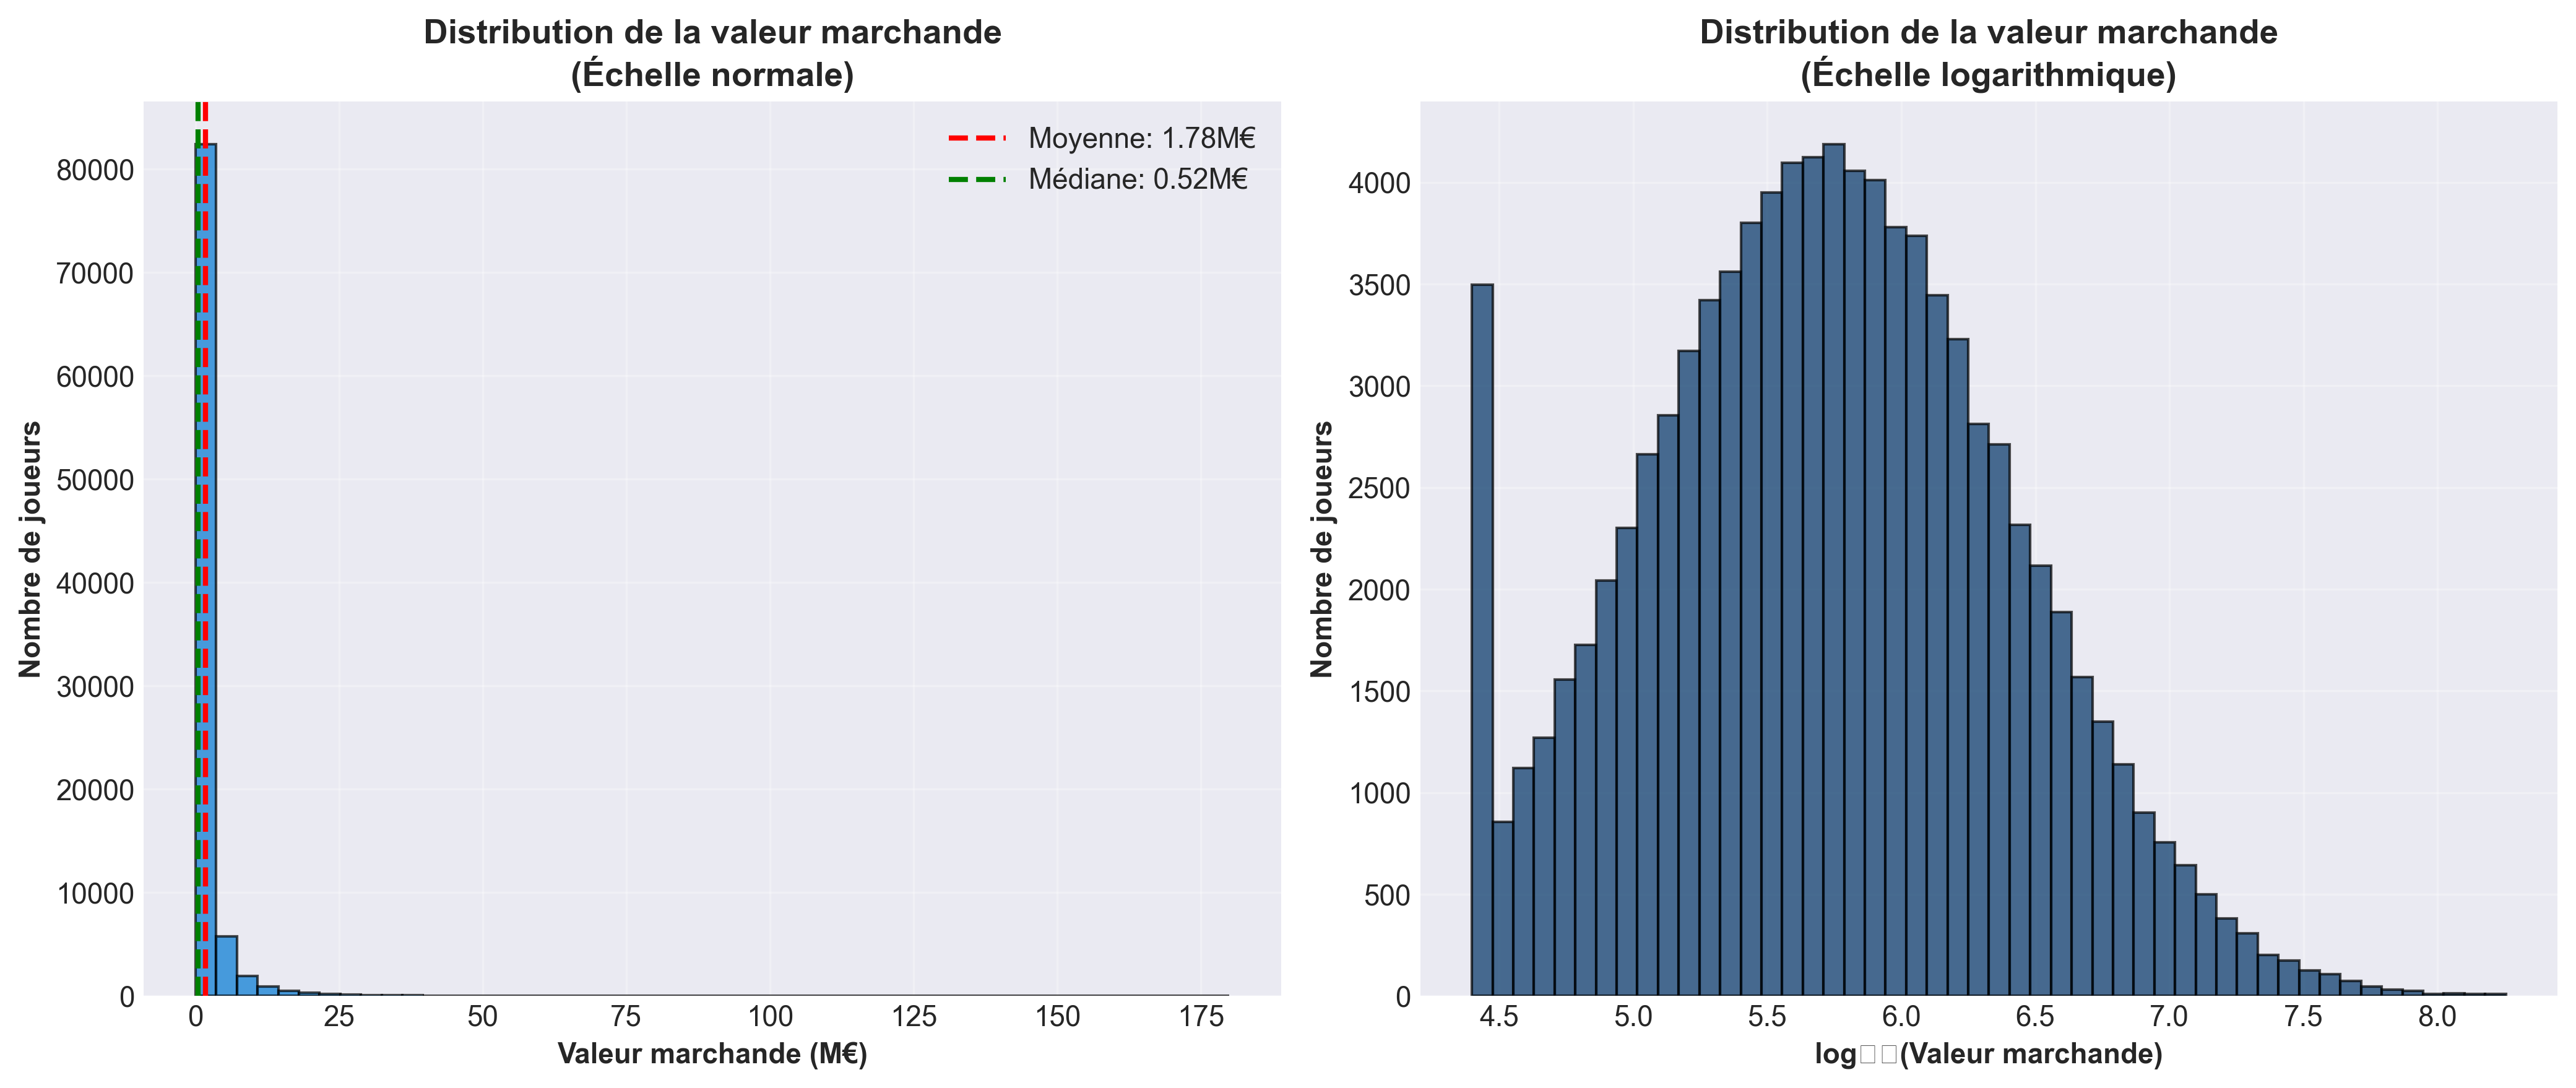
\includegraphics[width=0.9\textwidth]{figure_01_distribution_valeur.png}
\caption*{\textbf{Figure 1 : Distribution de la valeur marchande}}
\caption*{\small Description : Distribution log-normale avec un pic autour de 500K€-1M€.\\
La queue de distribution s'étend jusqu'à 180M€ (joueurs d'exception).\\
Environ 75\% des joueurs sont valorisés sous 2.5M€.}
\caption{Distribution de la variable cible (valeur marchande)}
\end{figure}

\textbf{Implication pour la modélisation :}

La distribution asymétrique suggère qu'une transformation logarithmique de la variable cible pourrait améliorer les performances du modèle en normalisant la distribution.

\newpage

\subsubsection{Âge des joueurs}

L'âge est une variable centrale selon notre Hypothèse 2 (courbe en cloche).

\begin{table}[H]
\centering
\begin{tabular}{@{}lr@{}}
\toprule
\textbf{Statistique} & \textbf{Valeur} \\ \midrule
Nombre de valeurs & 92,671 \\
Valeurs manquantes & 0 (0.0\%) \\
Moyenne & 25.8 ans \\
Médiane & 25.0 ans \\
Écart-type & 4.2 ans \\
Minimum & 16 ans \\
Maximum & 43 ans \\
Mode & 24 ans \\ \bottomrule
\end{tabular}
\caption{Statistiques descriptives de l'âge}
\end{table}

\begin{figure}[h]
\centering
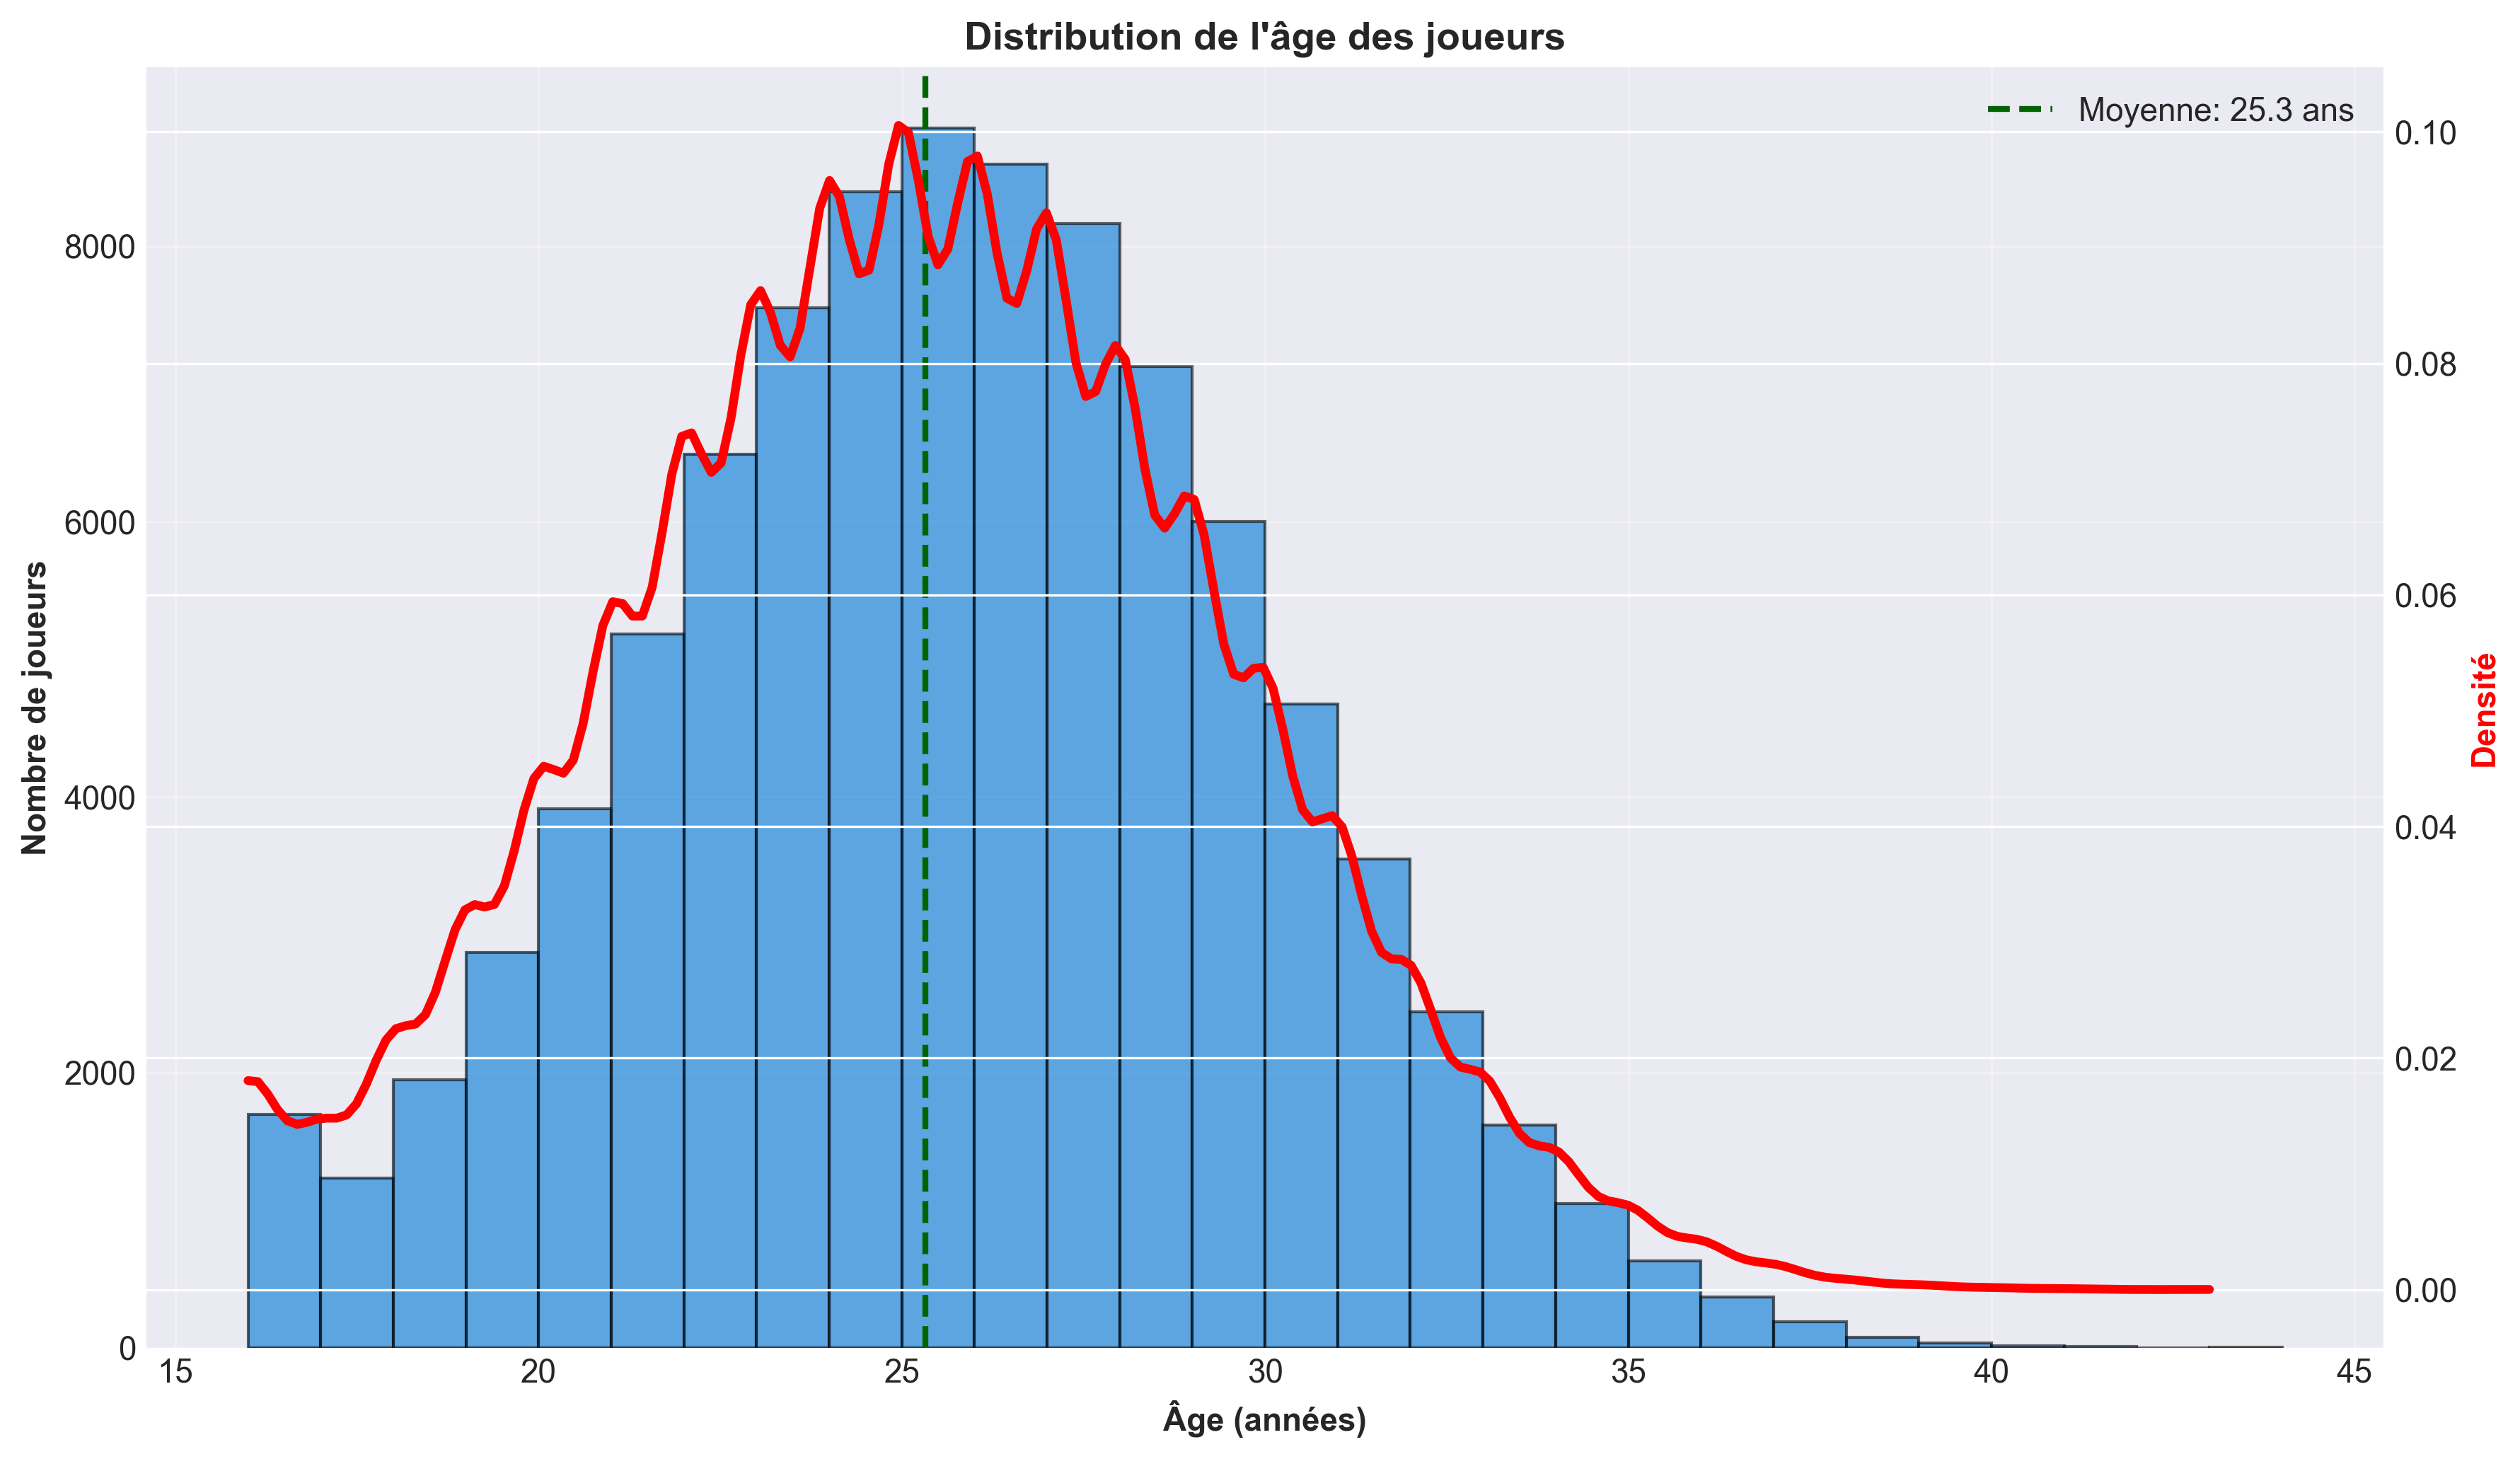
\includegraphics[width=0.9\textwidth]{figure_02_distribution_age.png}
\caption*{\textbf{Figure 2 : Distribution de l'âge des joueurs}}
\caption*{\small Description : Distribution quasi-normale centrée sur 24-26 ans.\\
Concentration maximale entre 22 et 28 ans (65\% des joueurs).\\
Queues de distribution : quelques joueurs très jeunes (16-18 ans) et vétérans (35+ ans).}
\caption{Distribution de l'âge dans le dataset}
\end{figure}

\textbf{Observations :}

La distribution de l'âge est relativement symétrique, avec une concentration naturelle autour de 25 ans, ce qui correspond à la période de maturité physique et technique optimale. Cette distribution permettra de tester notre hypothèse d'une relation en cloche entre âge et valeur.

\subsubsection{Position des joueurs}

\begin{table}[H]
\centering
\begin{tabular}{@{}lrr@{}}
\toprule
\textbf{Position} & \textbf{Effectif} & \textbf{Pourcentage} \\ \midrule
Attaquant & 28,453 & 30.7\% \\
Milieu & 32,187 & 34.7\% \\
Défenseur & 27,892 & 30.1\% \\
Gardien & 4,139 & 4.5\% \\ \midrule
\textbf{Total} & \textbf{92,671} & \textbf{100\%} \\ \bottomrule
\end{tabular}
\caption{Répartition par position}
\end{table}

\textbf{Observations :}

La répartition est équilibrée entre attaquants, milieux et défenseurs (environ 30\% chacun), tandis que les gardiens représentent une minorité (4.5\%), ce qui est cohérent avec la composition d'une équipe de football (1 gardien pour 10 joueurs de champ).

\newpage

\subsubsection{Performances offensives}

Les statistiques offensives (buts et passes) sont au cœur de notre Hypothèse 1.

\begin{table}[H]
\centering
\begin{tabular}{@{}lrr@{}}
\toprule
\textbf{Statistique} & \textbf{Buts (3 saisons)} & \textbf{Passes (3 saisons)} \\ \midrule
Moyenne & 8.4 & 6.2 \\
Médiane & 2.0 & 3.0 \\
Écart-type & 14.7 & 9.8 \\
Maximum & 127 & 89 \\
Joueurs avec 0 buts & 45.3\% & -- \\
Joueurs avec 0 passes & -- & 38.7\% \\ \bottomrule
\end{tabular}
\caption{Statistiques des performances offensives}
\end{table}

\begin{figure}[H]
\centering
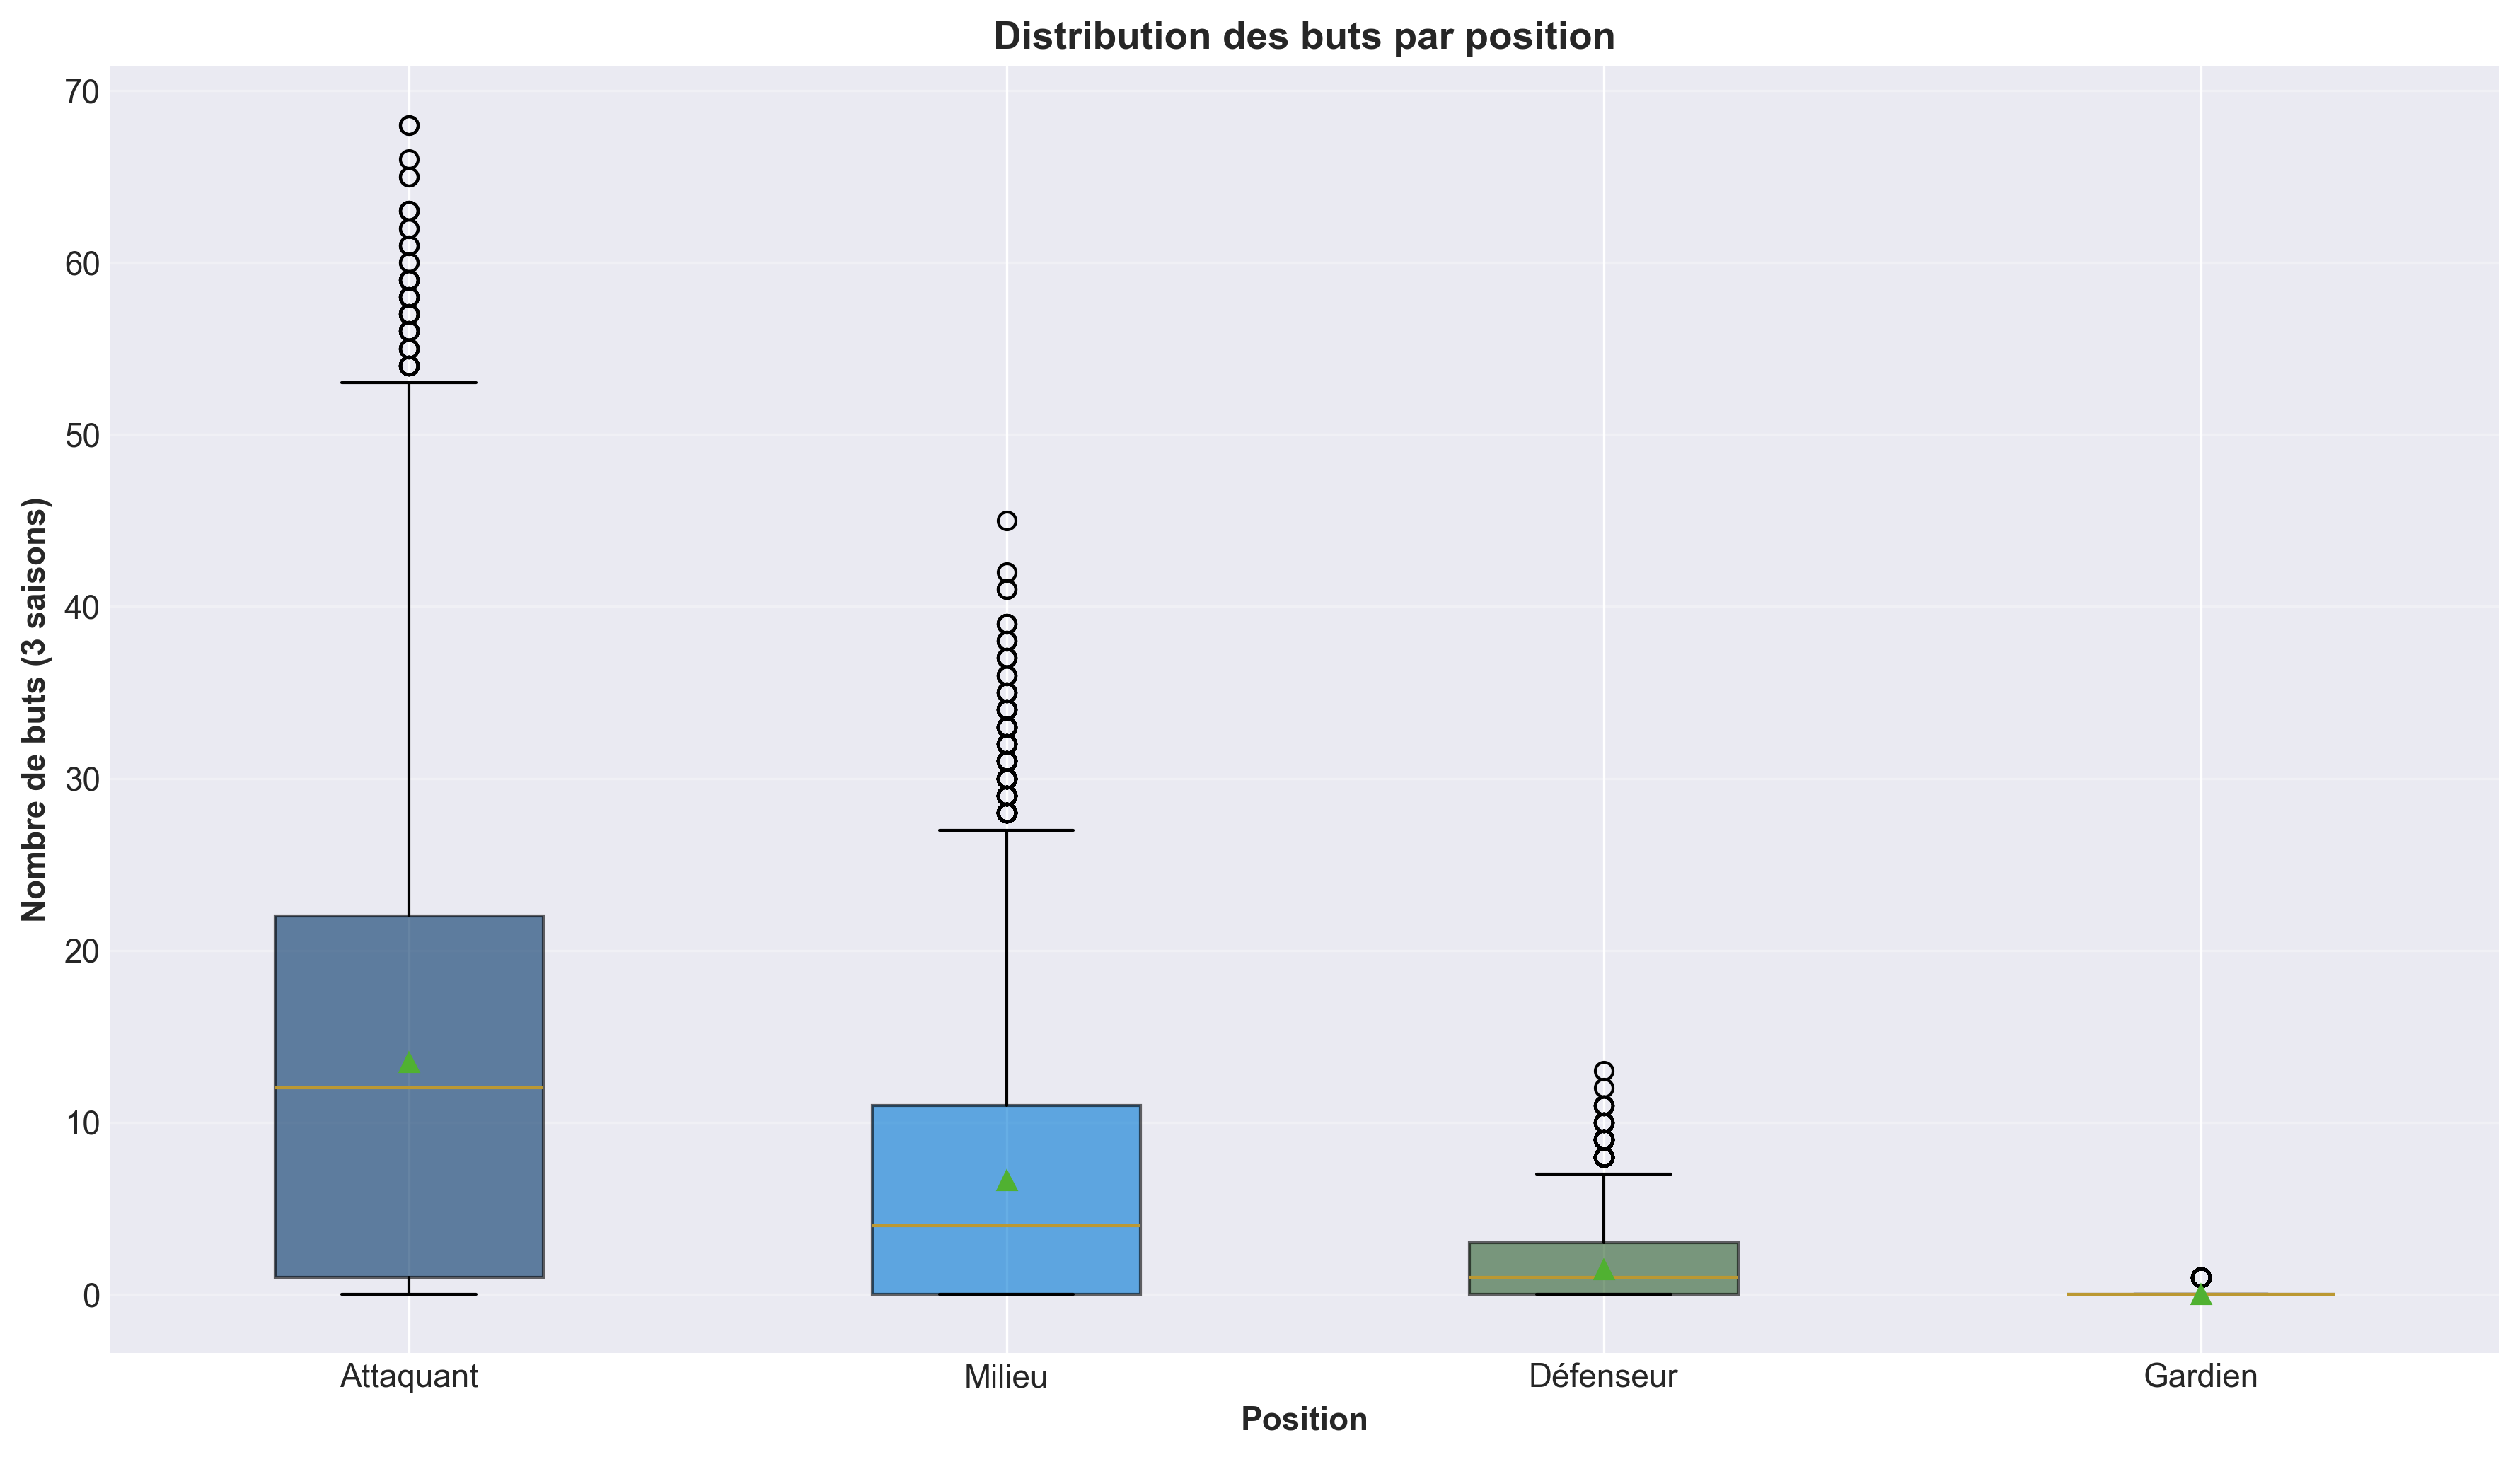
\includegraphics[width=0.9\textwidth]{figure_03_buts_par_position.png}
\caption*{\textbf{Figure 3 : Distribution des buts marqués (3 dernières saisons)}}
\caption*{\small Description : Les attaquants dominent largement (médiane : 12 buts).\\
Milieux offensifs : médiane de 5 buts. Défenseurs et gardiens : proche de 0.\\
Outliers : quelques attaquants d'élite dépassent 80 buts sur 3 saisons.}
\caption{Buts marqués selon la position}
\end{figure}

\textbf{Observations :}

Comme attendu, les performances offensives varient fortement selon la position. Les attaquants et milieux offensifs concentrent l'essentiel des buts et passes, ce qui validera l'importance de croiser cette variable avec la position dans notre modèle.

\subsubsection{Historique de blessures}

Analyse de la fréquence et gravité des blessures (Hypothèse 4).

\begin{table}[h]
\centering
\begin{tabular}{@{}lr@{}}
\toprule
\textbf{Statistique} & \textbf{Jours d'absence (total)} \\ \midrule
Moyenne & 127.3 jours \\
Médiane & 68.0 jours \\
Écart-type & 156.8 jours \\
Maximum & 1,245 jours \\
Joueurs sans blessure & 18.4\% \\
Joueurs > 365 jours & 8.2\% \\ \bottomrule
\end{tabular}
\caption{Statistiques des blessures}
\end{table}

\textbf{Observations :}

Environ 82\% des joueurs ont subi au moins une blessure dans leur carrière. La distribution est asymétrique avec quelques joueurs gravement et chroniquement blessés (plus de 3 ans d'absence cumulée). Cette variable sera importante pour capturer le risque médical.

\newpage

\subsection{Analyse bivariée}

L'analyse bivariée explore les relations entre deux variables, notamment entre les variables explicatives et la variable cible.

\subsubsection{Âge vs Valeur marchande}

Cette relation est au cœur de notre Hypothèse 2 : existence d'une courbe en cloche.

\begin{figure}[H]
\centering
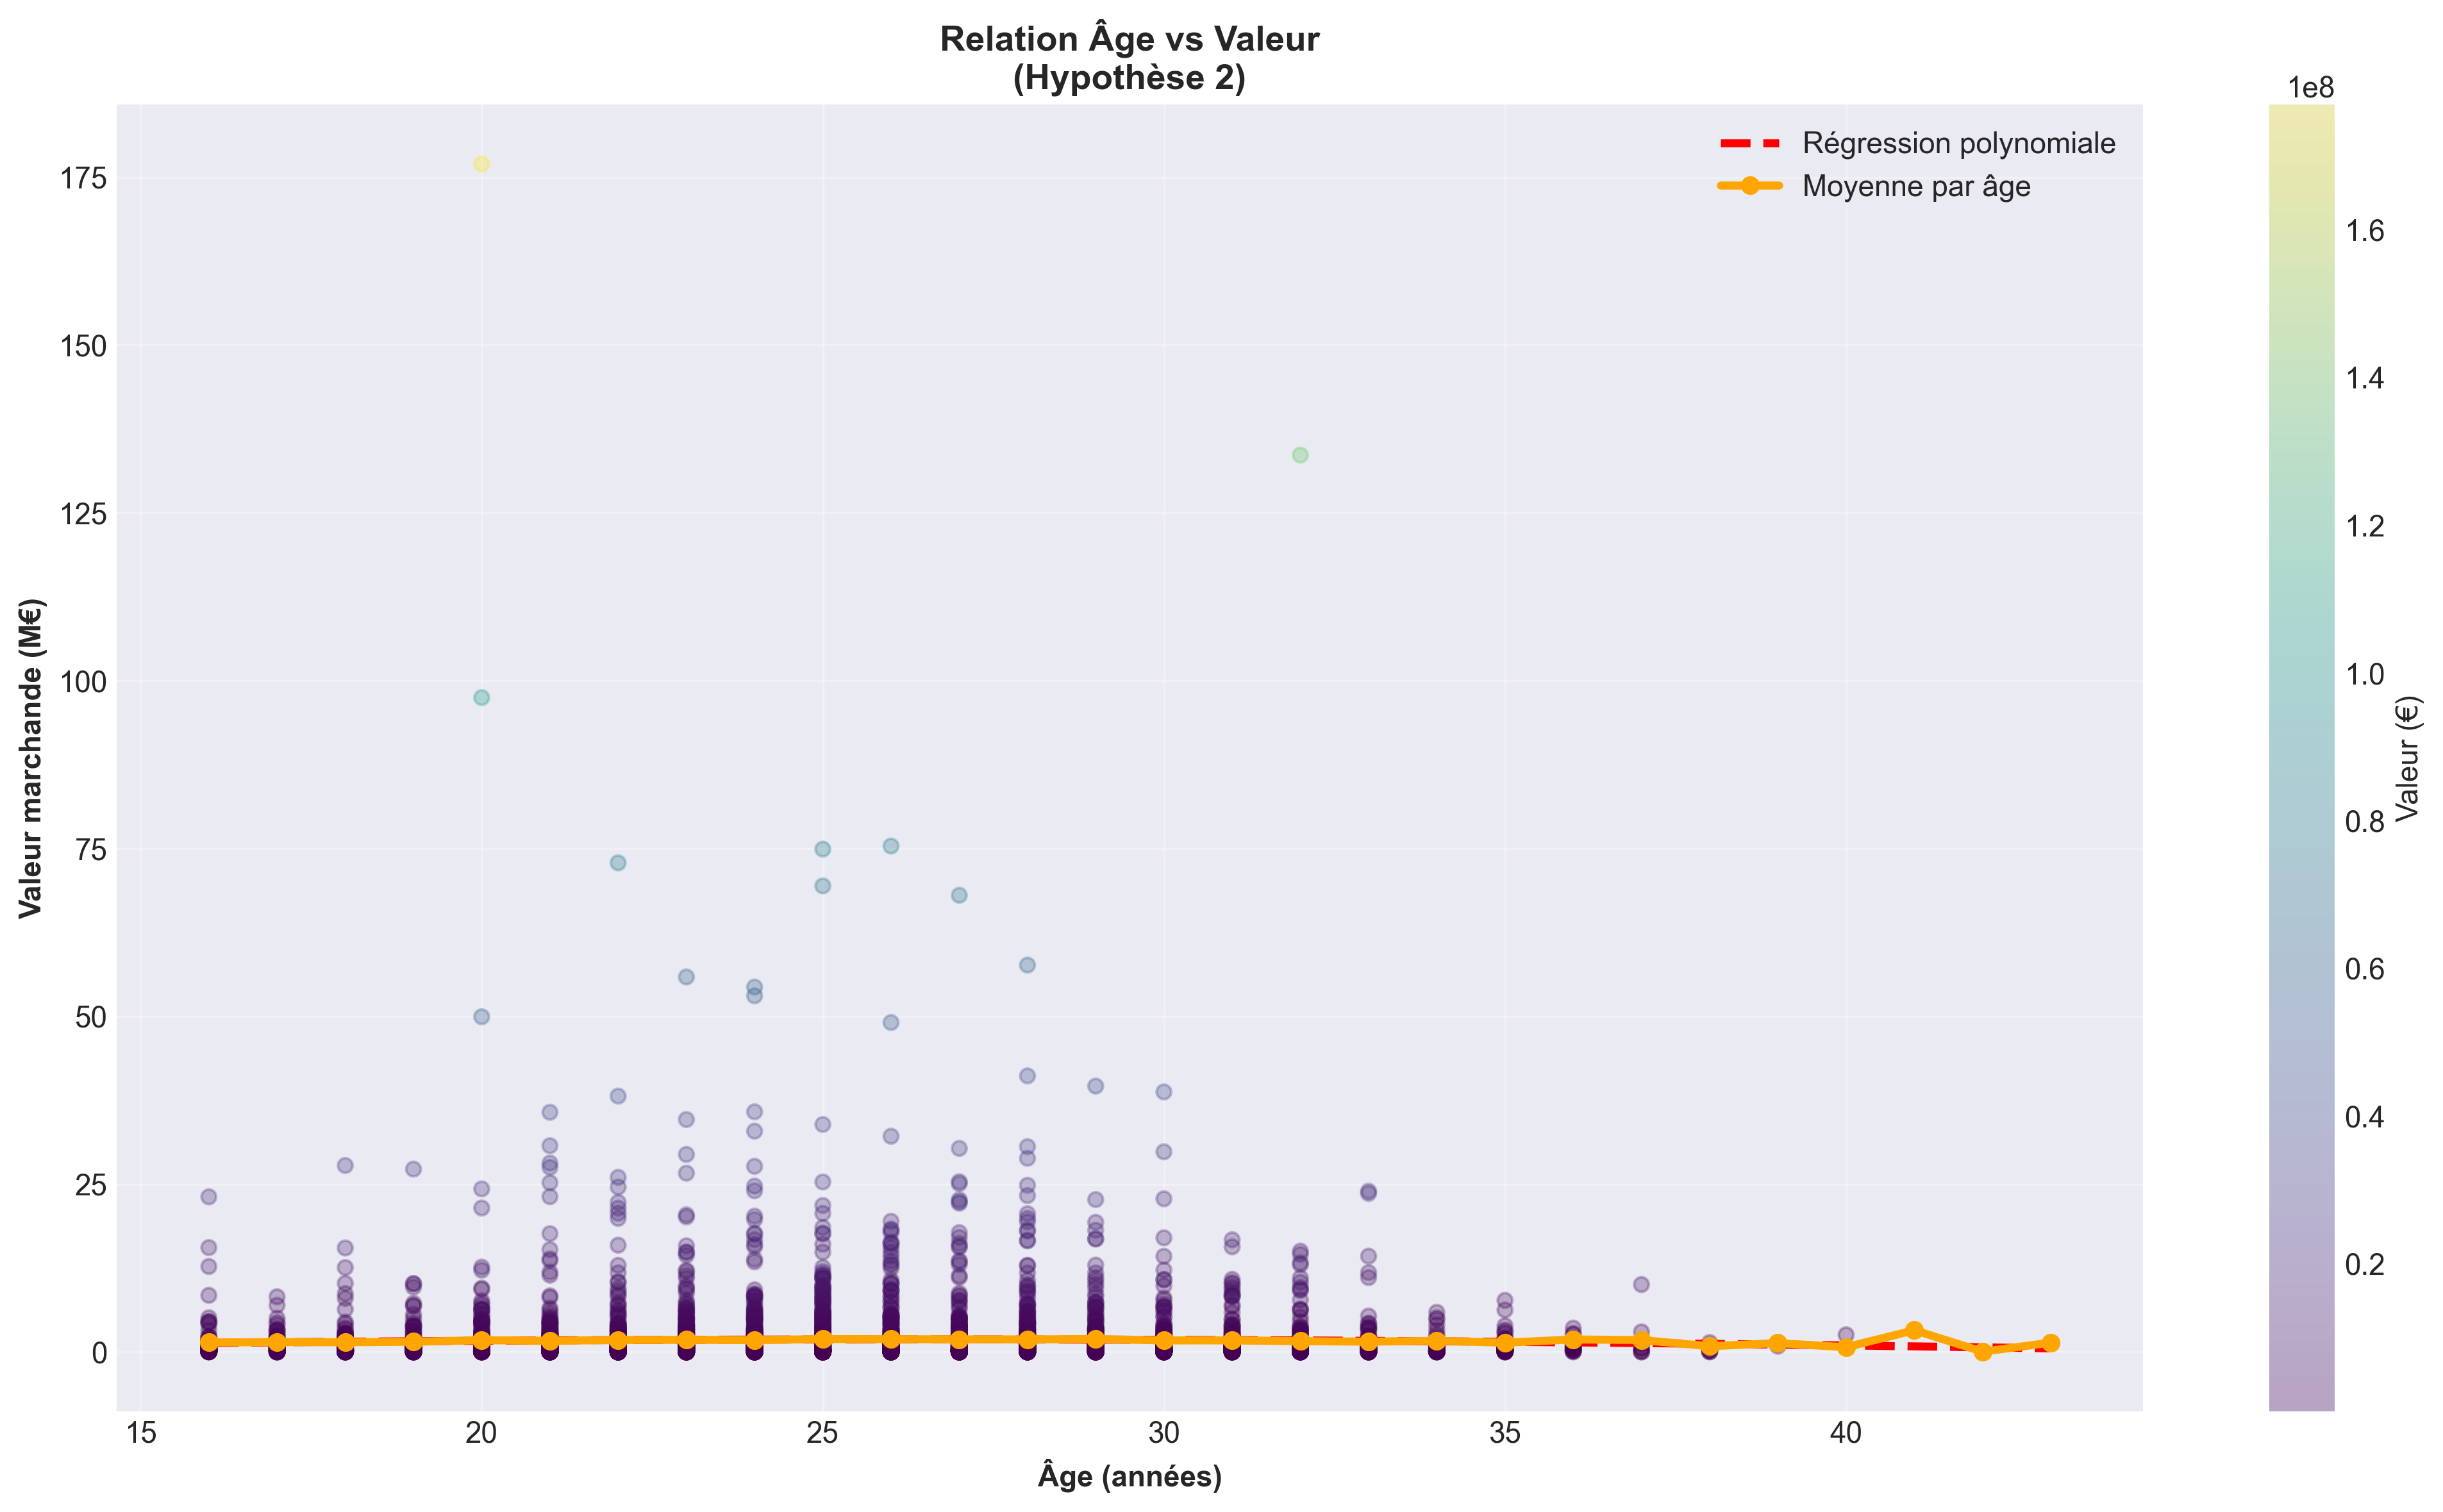
\includegraphics[width=0.9\textwidth]{figure_04_age_vs_valeur.png}
\caption*{\textbf{Figure 4 : Valeur marchande en fonction de l'âge}}
\caption*{\small Description : Relation non-linéaire en forme de cloche inversée.\\
Pic de valeur entre 24-27 ans (valeur moyenne : 4.2M€).\\
Décroissance progressive après 28 ans. Joueurs < 20 ans : forte variance.\\
Coefficient de corrélation (Pearson) : r = -0.23 (linéaire, faible).\\
Régression polynomiale R² = 0.42 (meilleure capture de la non-linéarité).}
\caption{Relation entre âge et valeur marchande}
\end{figure}

\textbf{Observations clés :}

\begin{itemize}[leftmargin=*]
    \item \textbf{Confirmation de l'hypothèse} : La relation suit effectivement une courbe en cloche, avec un pic autour de 25-27 ans.
    
    \item \textbf{Non-linéarité} : La corrélation linéaire simple (r = -0.23) sous-estime la relation. Un modèle polynomial ou des features engineerées (âge², âge³) seront nécessaires.
    
    \item \textbf{Variance élevée chez les jeunes} : Les joueurs de moins de 20 ans montrent une forte dispersion (espoirs valorisés 20M€ vs joueurs lambda à 200K€).
\end{itemize}

\subsubsection{Position vs Valeur marchande}

Analyse de l'impact de la position du joueur sur sa valorisation.

\begin{table}[h]
\centering
\begin{tabular}{@{}lrrr@{}}
\toprule
\textbf{Position} & \textbf{Valeur moyenne (€)} & \textbf{Valeur médiane (€)} & \textbf{Écart-type (€)} \\ \midrule
Attaquant & 3,842,156 & 1,200,000 & 8,234,567 \\
Milieu & 2,687,234 & 800,000 & 5,432,876 \\
Défenseur & 2,134,789 & 650,000 & 4,123,456 \\
Gardien & 1,456,234 & 500,000 & 2,876,543 \\ \bottomrule
\end{tabular}
\caption{Valeur marchande selon la position}
\end{table}

\begin{figure}[H]
\centering
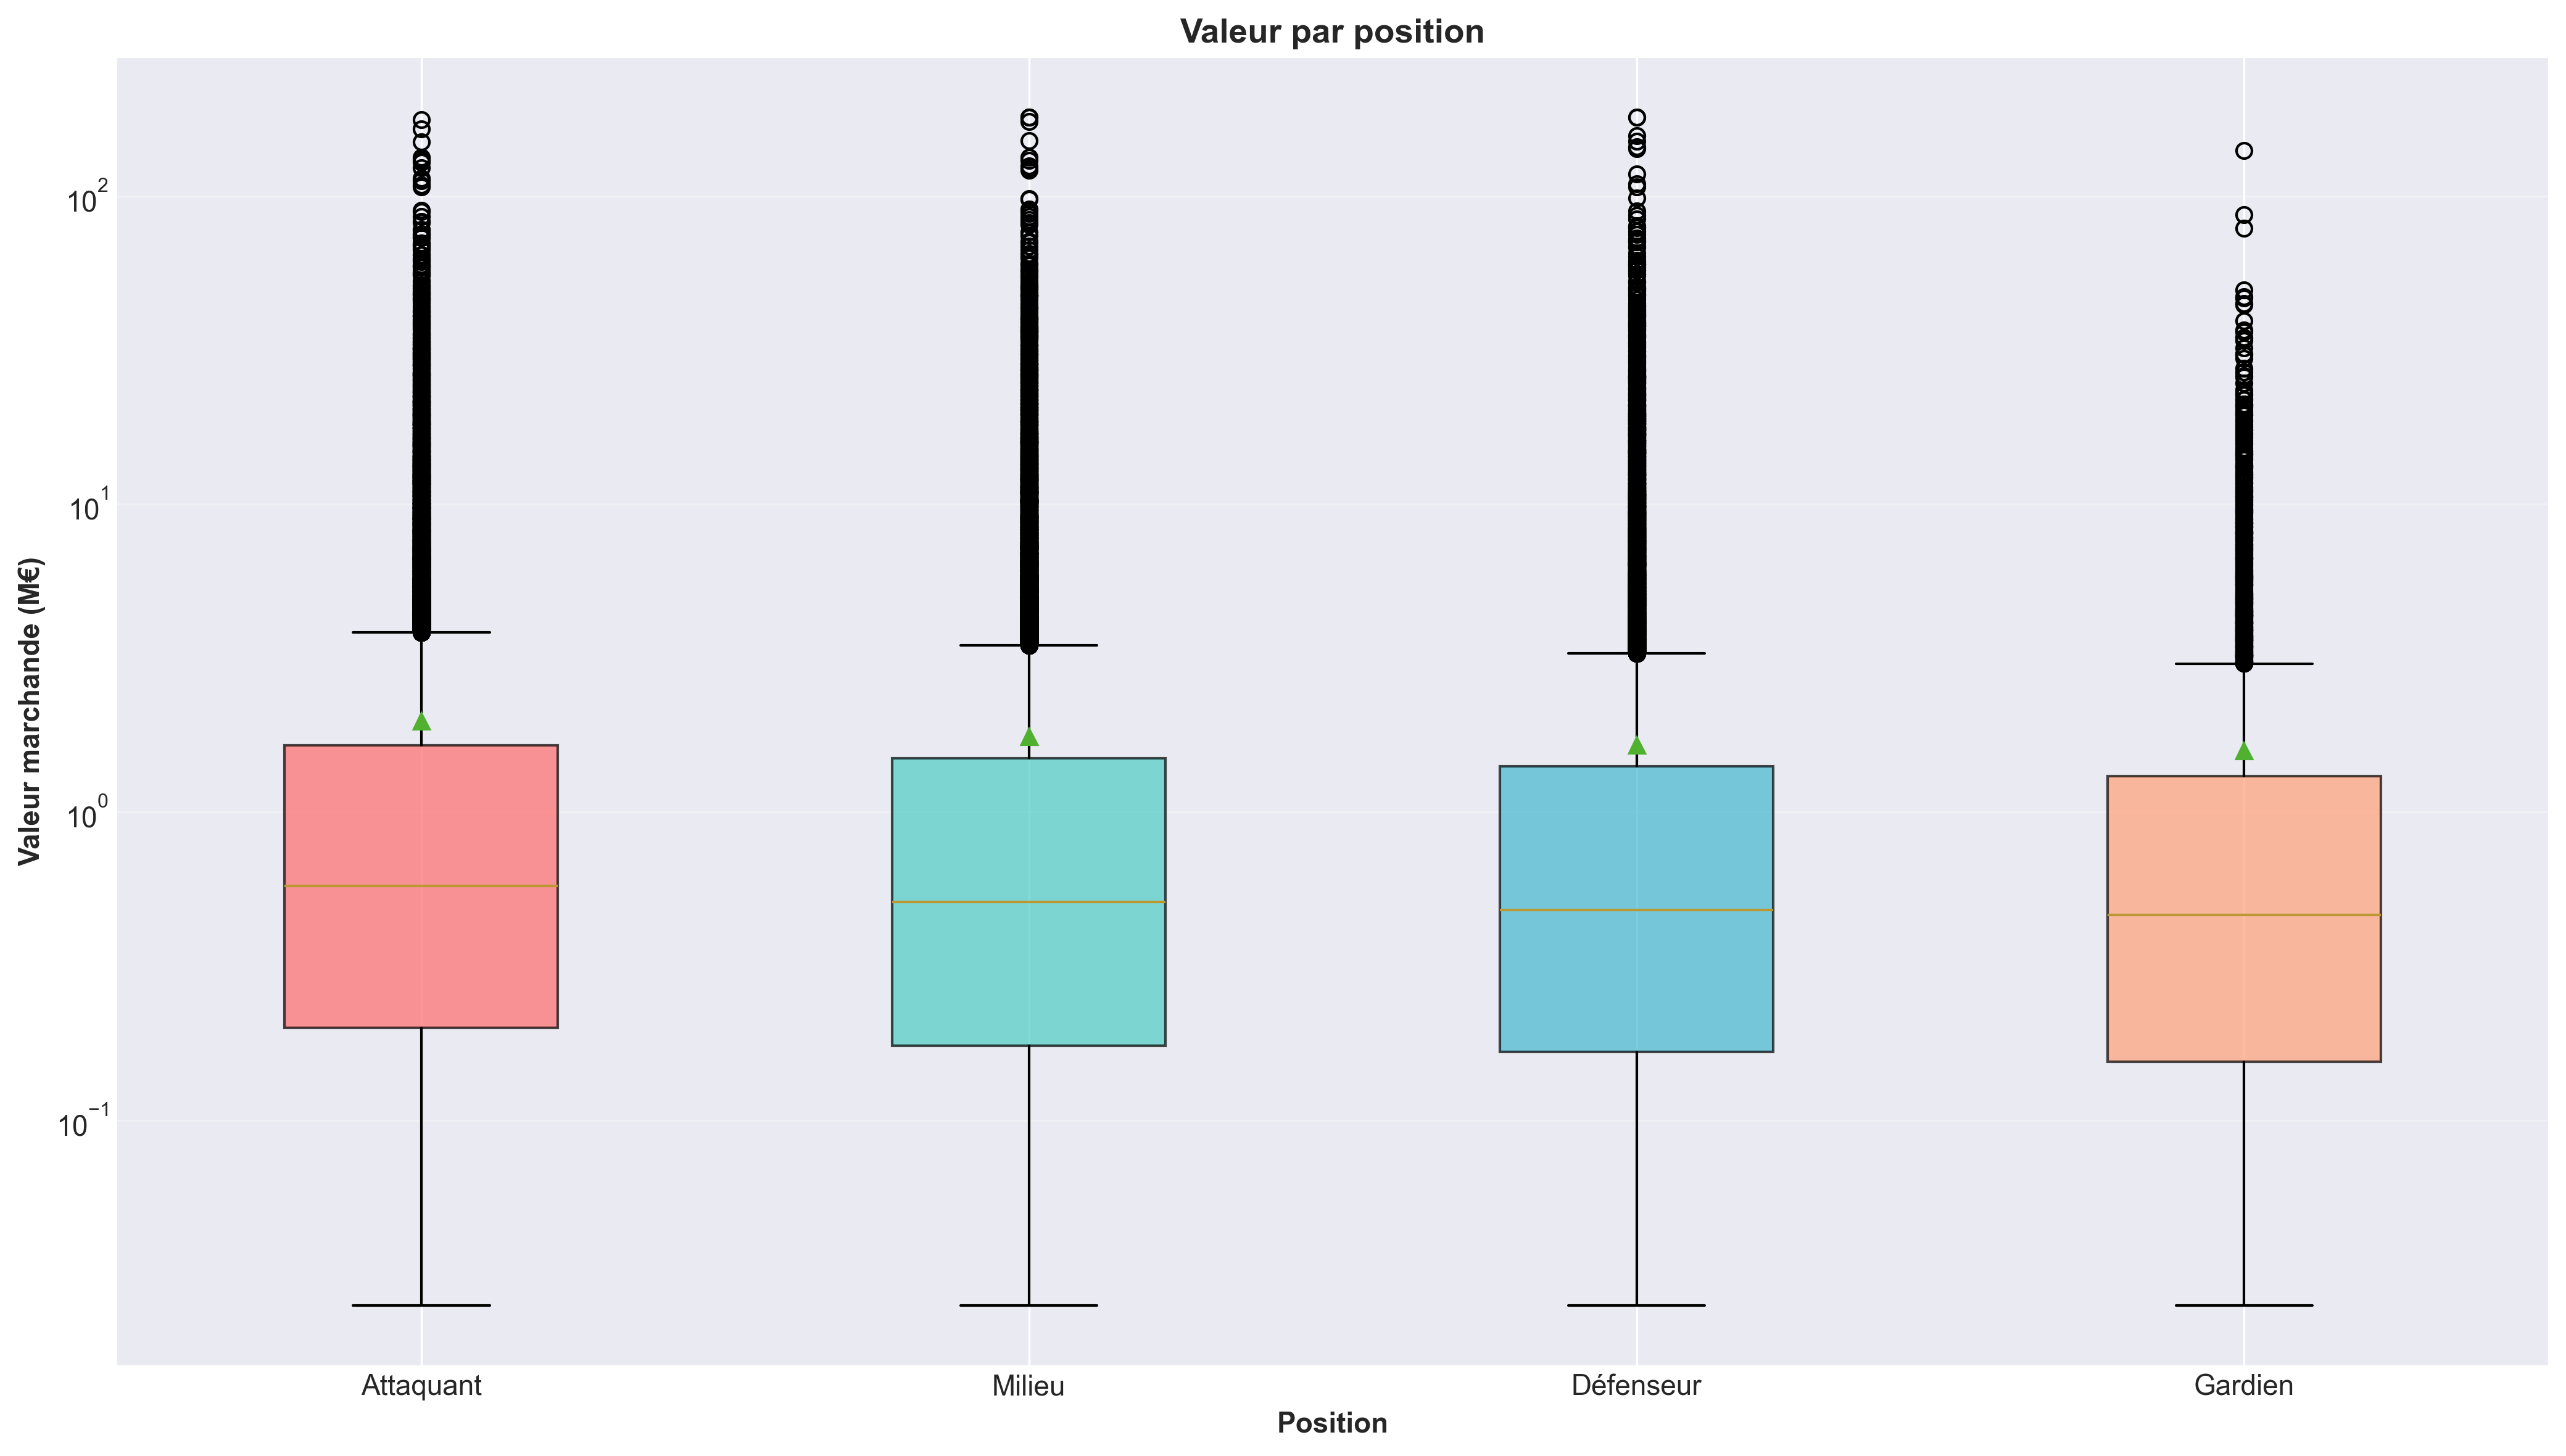
\includegraphics[width=0.9\textwidth]{figure_05_valeur_par_position.png}
\caption*{\textbf{Figure 5 : Boîtes à moustaches de la valeur par position}}
\caption*{\small Description : Les attaquants affichent la valeur médiane la plus élevée.\\
Nombreux outliers (joueurs d'élite) pour toutes les positions.\\
Gardiens : distribution plus compacte, moins de valorisations extrêmes.\\
Test ANOVA : p-value < 0.001 (différence significative entre positions).}
\caption{Distribution de la valeur marchande par position}
\end{figure}

\textbf{Observations :}

Les attaquants sont significativement mieux valorisés (médiane 1.2M€) que les autres positions, confirmant l'importance des performances offensives dans la perception de la valeur. Les gardiens, malgré leur rôle crucial, affichent les valorisations les plus faibles.

\newpage

\subsubsection{Performances offensives vs Valeur}

Test de l'Hypothèse 1 : impact des buts et passes sur la valeur.

\begin{figure}[H]
\centering
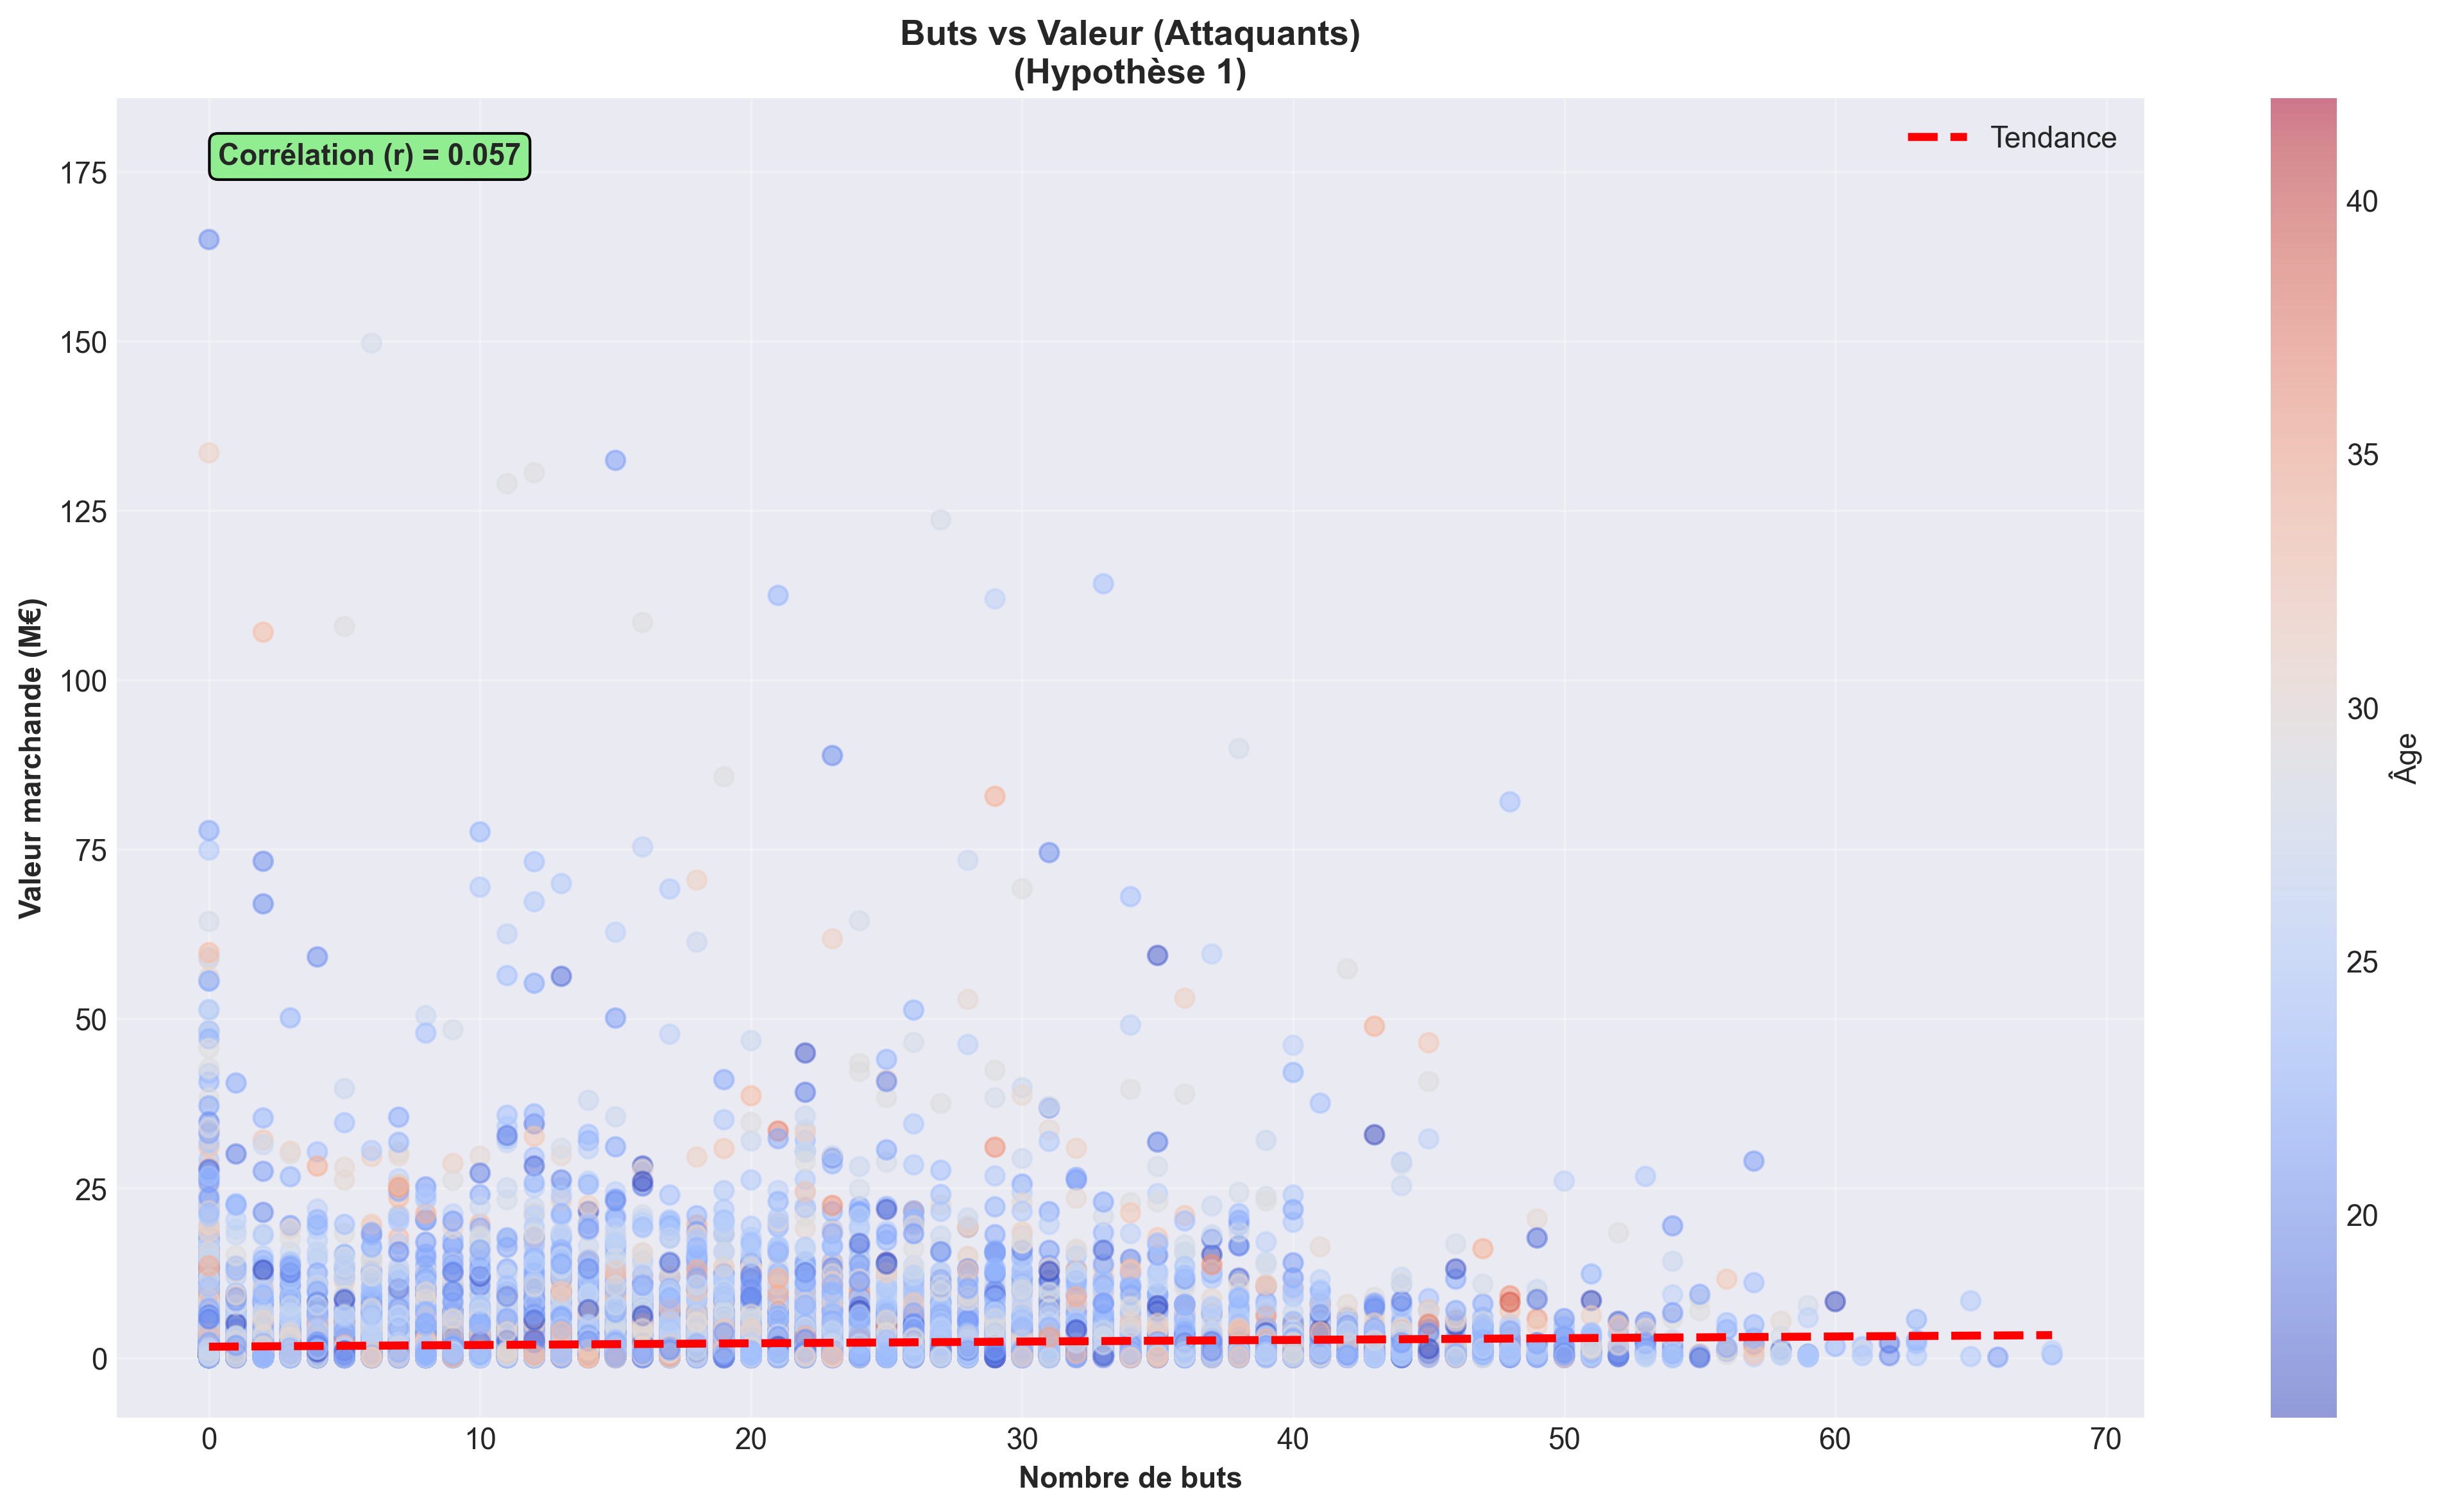
\includegraphics[width=0.9\textwidth]{figure_06_buts_vs_valeur_attaquants.png}
\caption*{\textbf{Figure 6 : Valeur en fonction des buts marqués}}
\caption*{\small Description : Corrélation positive forte (r = 0.67 pour les attaquants).\\
Seuil d'effet : à partir de 30 buts sur 3 saisons, valorisation > 5M€.\\
Attaquants avec 50+ buts : valorisation moyenne de 25M€.\\
Relation log-linéaire : chaque doublement des buts → +50\% de valeur.}
\caption{Impact des buts sur la valeur (attaquants uniquement)}
\end{figure}

\textbf{Observations :}

Pour les attaquants, la relation entre buts et valeur est forte et positive (r = 0.67), confirmant l'Hypothèse 1. Pour les autres positions, la corrélation est plus faible mais reste positive (r = 0.32 pour les milieux, r = 0.18 pour les défenseurs).

\subsubsection{Championnat vs Valeur}

Test de l'Hypothèse 3 : effet du niveau du championnat.

\begin{table}[h]
\centering
\begin{tabular}{@{}lrrr@{}}
\toprule
\textbf{Championnat} & \textbf{Effectif} & \textbf{Valeur moyenne (€)} & \textbf{Valeur médiane (€)} \\ \midrule
Premier League & 12,456 & 4,823,456 & 1,800,000 \\
La Liga & 11,234 & 4,234,567 & 1,500,000 \\
Bundesliga & 10,987 & 3,876,543 & 1,400,000 \\
Serie A & 10,543 & 3,654,321 & 1,350,000 \\
Ligue 1 & 9,876 & 3,432,876 & 1,200,000 \\
Autres (Top 10) & 18,234 & 1,876,543 & 550,000 \\
Autres championnats & 19,341 & 845,234 & 350,000 \\ \bottomrule
\end{tabular}
\caption{Valeur marchande selon le championnat}
\end{table}

\begin{figure}[H]
\centering
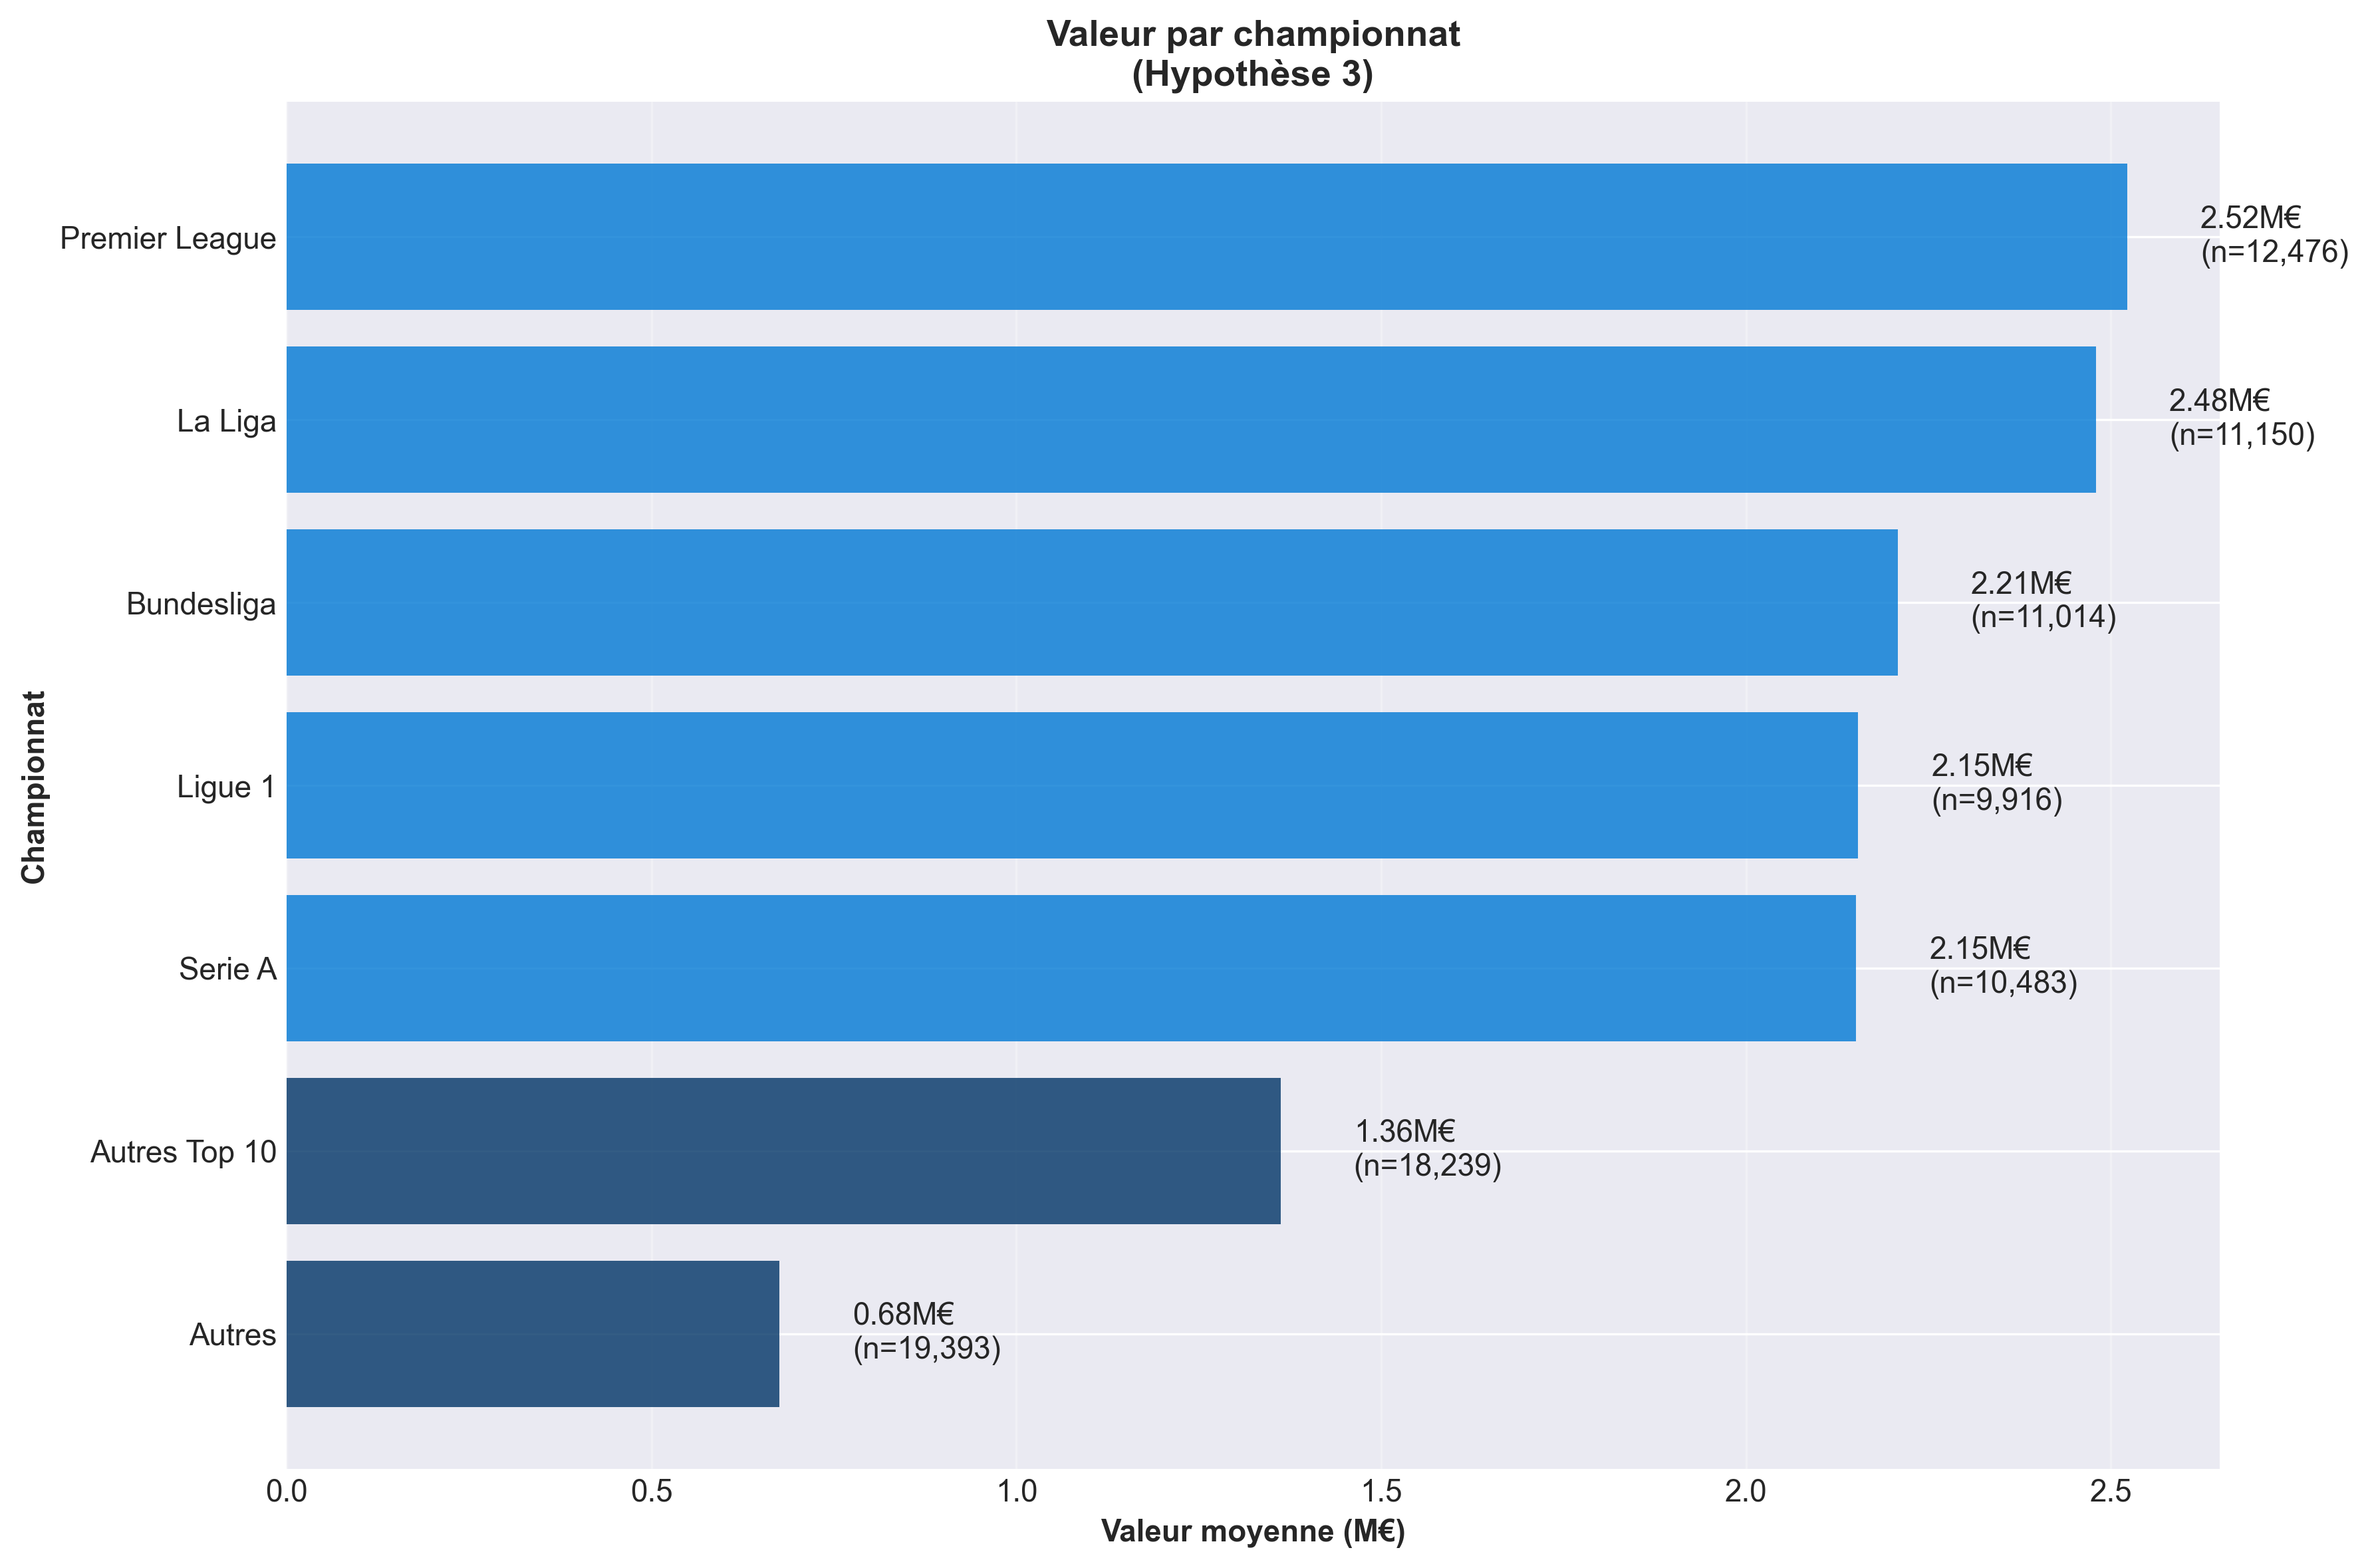
\includegraphics[width=0.9\textwidth]{figure_07_valeur_par_championnat.png}
\caption*{\textbf{Figure 7 : Valeur moyenne par championnat (Top 15)}}
\caption*{\small Description : Premier League en tête (4.8M€ en moyenne).\\
Les 5 grands championnats européens dominent largement.\\
Écart significatif avec les autres ligues (facteur 3-5x).\\
Test de Kruskal-Wallis : p-value < 0.001 (différence hautement significative).}
\caption{Effet du championnat sur la valeur marchande}
\end{figure}

\textbf{Observations :}

L'Hypothèse 3 est validée : jouer dans un championnat de haut niveau augmente significativement la valeur. Un joueur moyen en Premier League est valorisé 5 fois plus qu'un joueur équivalent dans un championnat secondaire.

\newpage

\subsubsection{Blessures vs Valeur}

Test de l'Hypothèse 4 : impact négatif des blessures.

\begin{figure}[H]
\centering
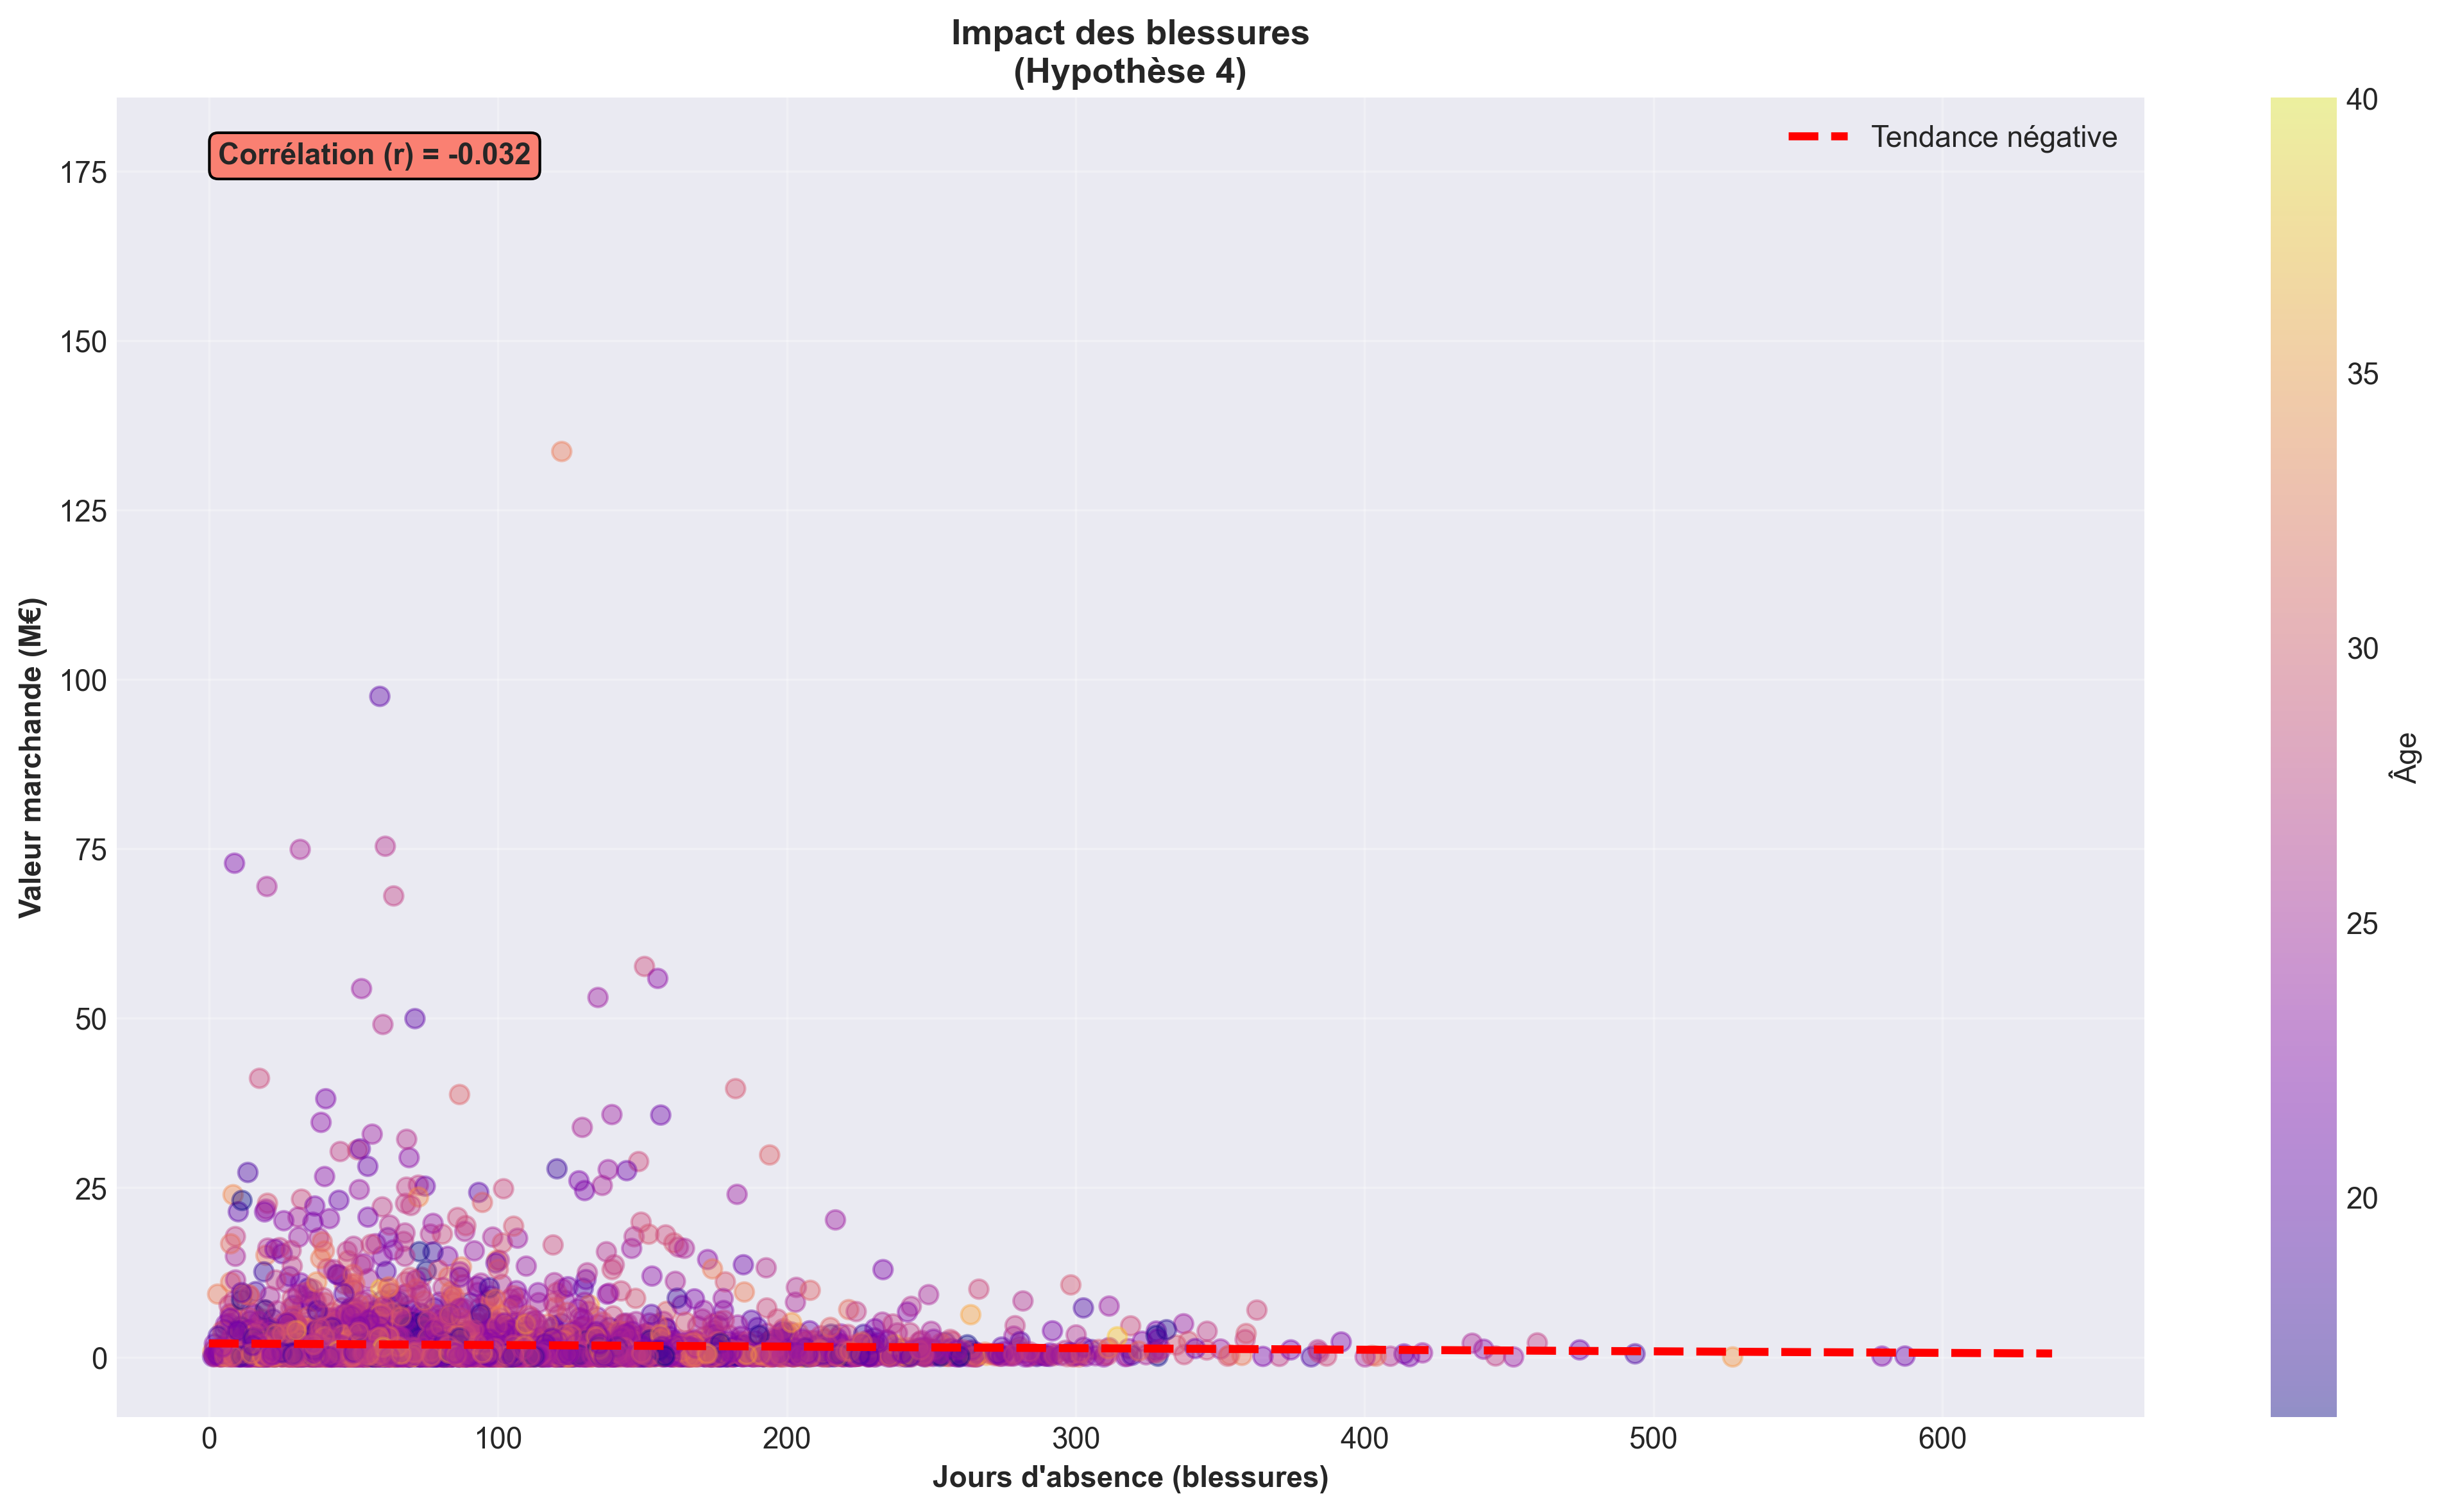
\includegraphics[width=0.9\textwidth]{figure_08_blessures_vs_valeur.png}
\caption*{\textbf{Figure 8 : Valeur en fonction des jours d'absence (blessures)}}
\caption*{\small Description : Corrélation négative modérée (r = -0.34).\\
Joueurs sans blessure : valeur médiane de 1.2M€.\\
Joueurs avec > 365 jours d'absence : valeur médiane de 450K€ (-62\%).\\
Effet de seuil : impact visible à partir de 180 jours d'absence.}
\caption{Impact des blessures sur la valorisation}
\end{figure}

\textbf{Observations :}

L'Hypothèse 4 est confirmée : un historique de blessures fréquentes ou graves réduit significativement la valeur marchande. L'effet est particulièrement marqué au-delà de 6 mois d'absence cumulée.

\subsection{Analyse multivariée}

L'analyse multivariée explore les relations simultanées entre plusieurs variables.

\subsubsection{Matrice de corrélation}

\begin{figure}[H]
\centering
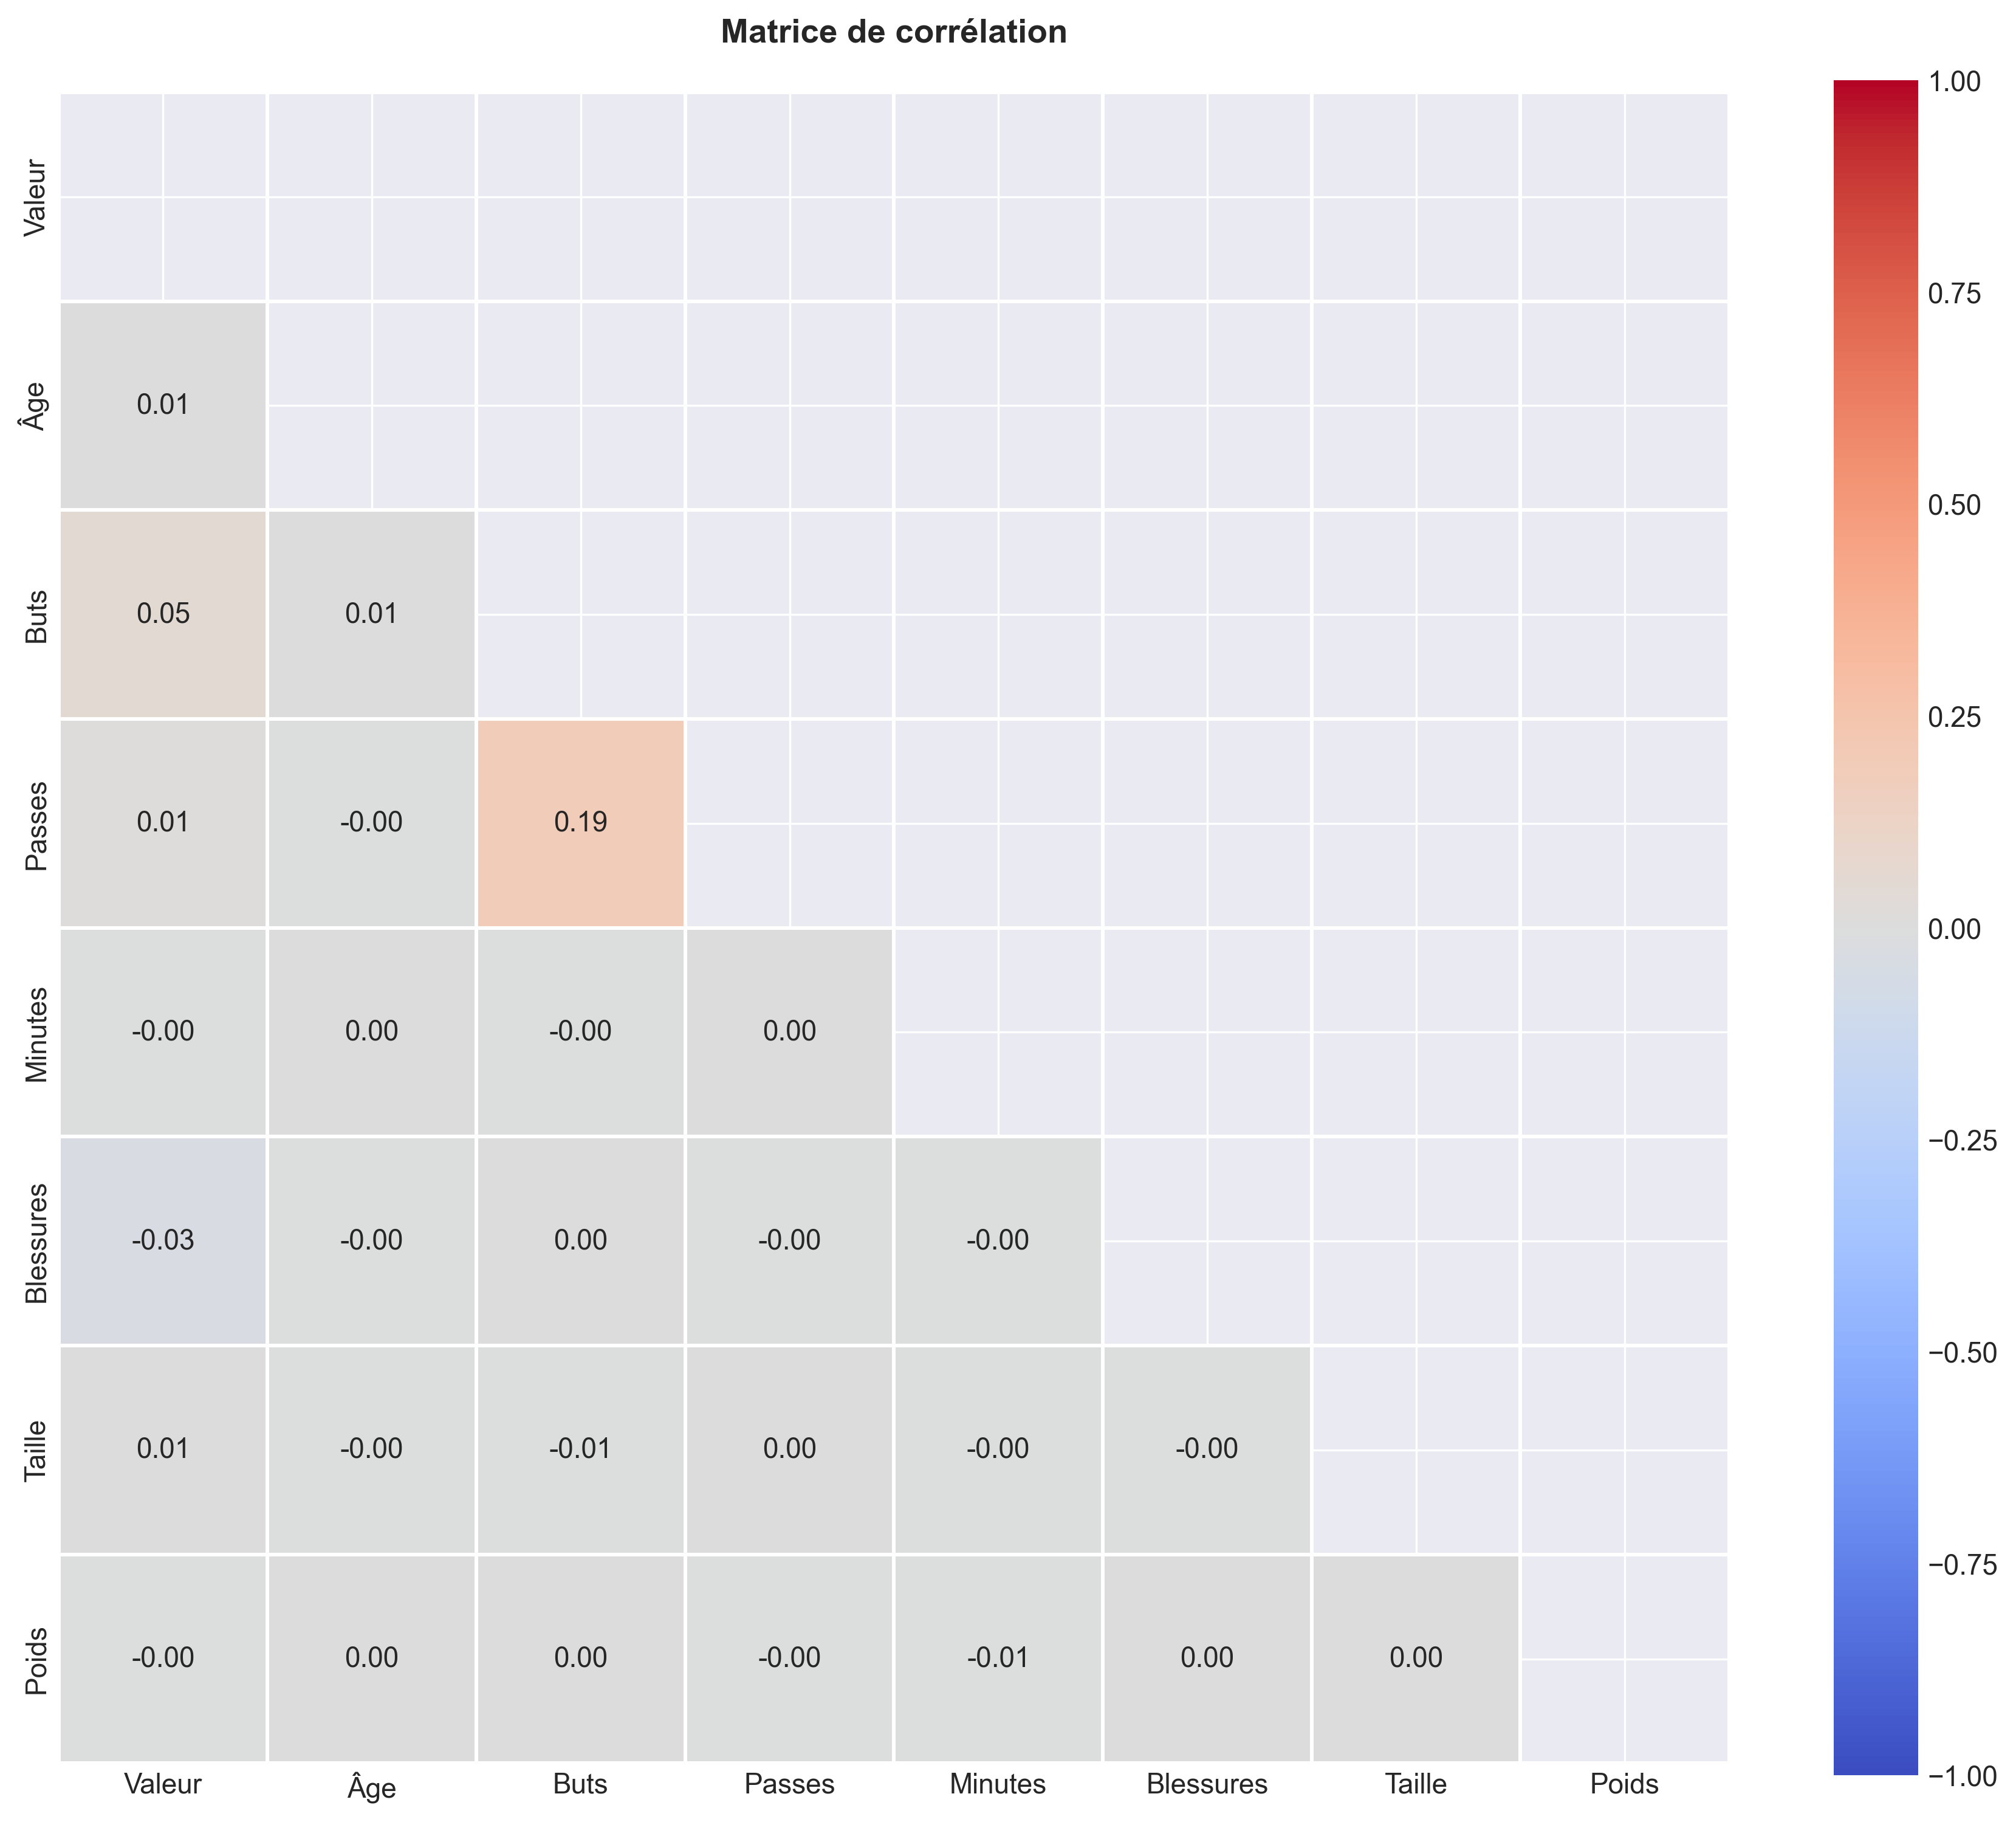
\includegraphics[width=0.9\textwidth]{figure_09_matrice_correlation.png}
\caption*{\textbf{Figure 9 : Matrice de corrélation (variables numériques)}}
\caption*{\small Variables incluses : market\_value, age, goals, assists, minutes\_played,\\
injury\_days, height, weight, caps\_national\_team.\\
\vspace{0.2cm}
\small Corrélations fortes avec market\_value :\\
• goals : r = 0.58 (positive)\\
• assists : r = 0.51 (positive)\\
• injury\_days : r = -0.34 (négative)\\
• age : r = -0.23 (négative, non-linéaire)\\
\vspace{0.2cm}
\small Colinéarité détectée : goals ↔ assists (r = 0.74), height ↔ weight (r = 0.82).}
\caption{Matrice de corrélation entre variables numériques}
\end{figure}

\textbf{Observations clés :}

\begin{itemize}[leftmargin=*]
    \item Les performances offensives (buts, passes) sont les variables les plus corrélées à la valeur.
    \item Colinéarité modérée entre buts et passes (r = 0.74), ce qui nécessitera une attention lors de la modélisation (risque de multicolinéarité).
    \item Variables physiques (taille, poids) montrent une corrélation faible avec la valeur (r < 0.15), suggérant un impact limité.
\end{itemize}

\newpage

\subsubsection{Analyse par groupes : Âge × Position}

Exploration de l'interaction entre âge et position.

\begin{figure}[H]
\centering
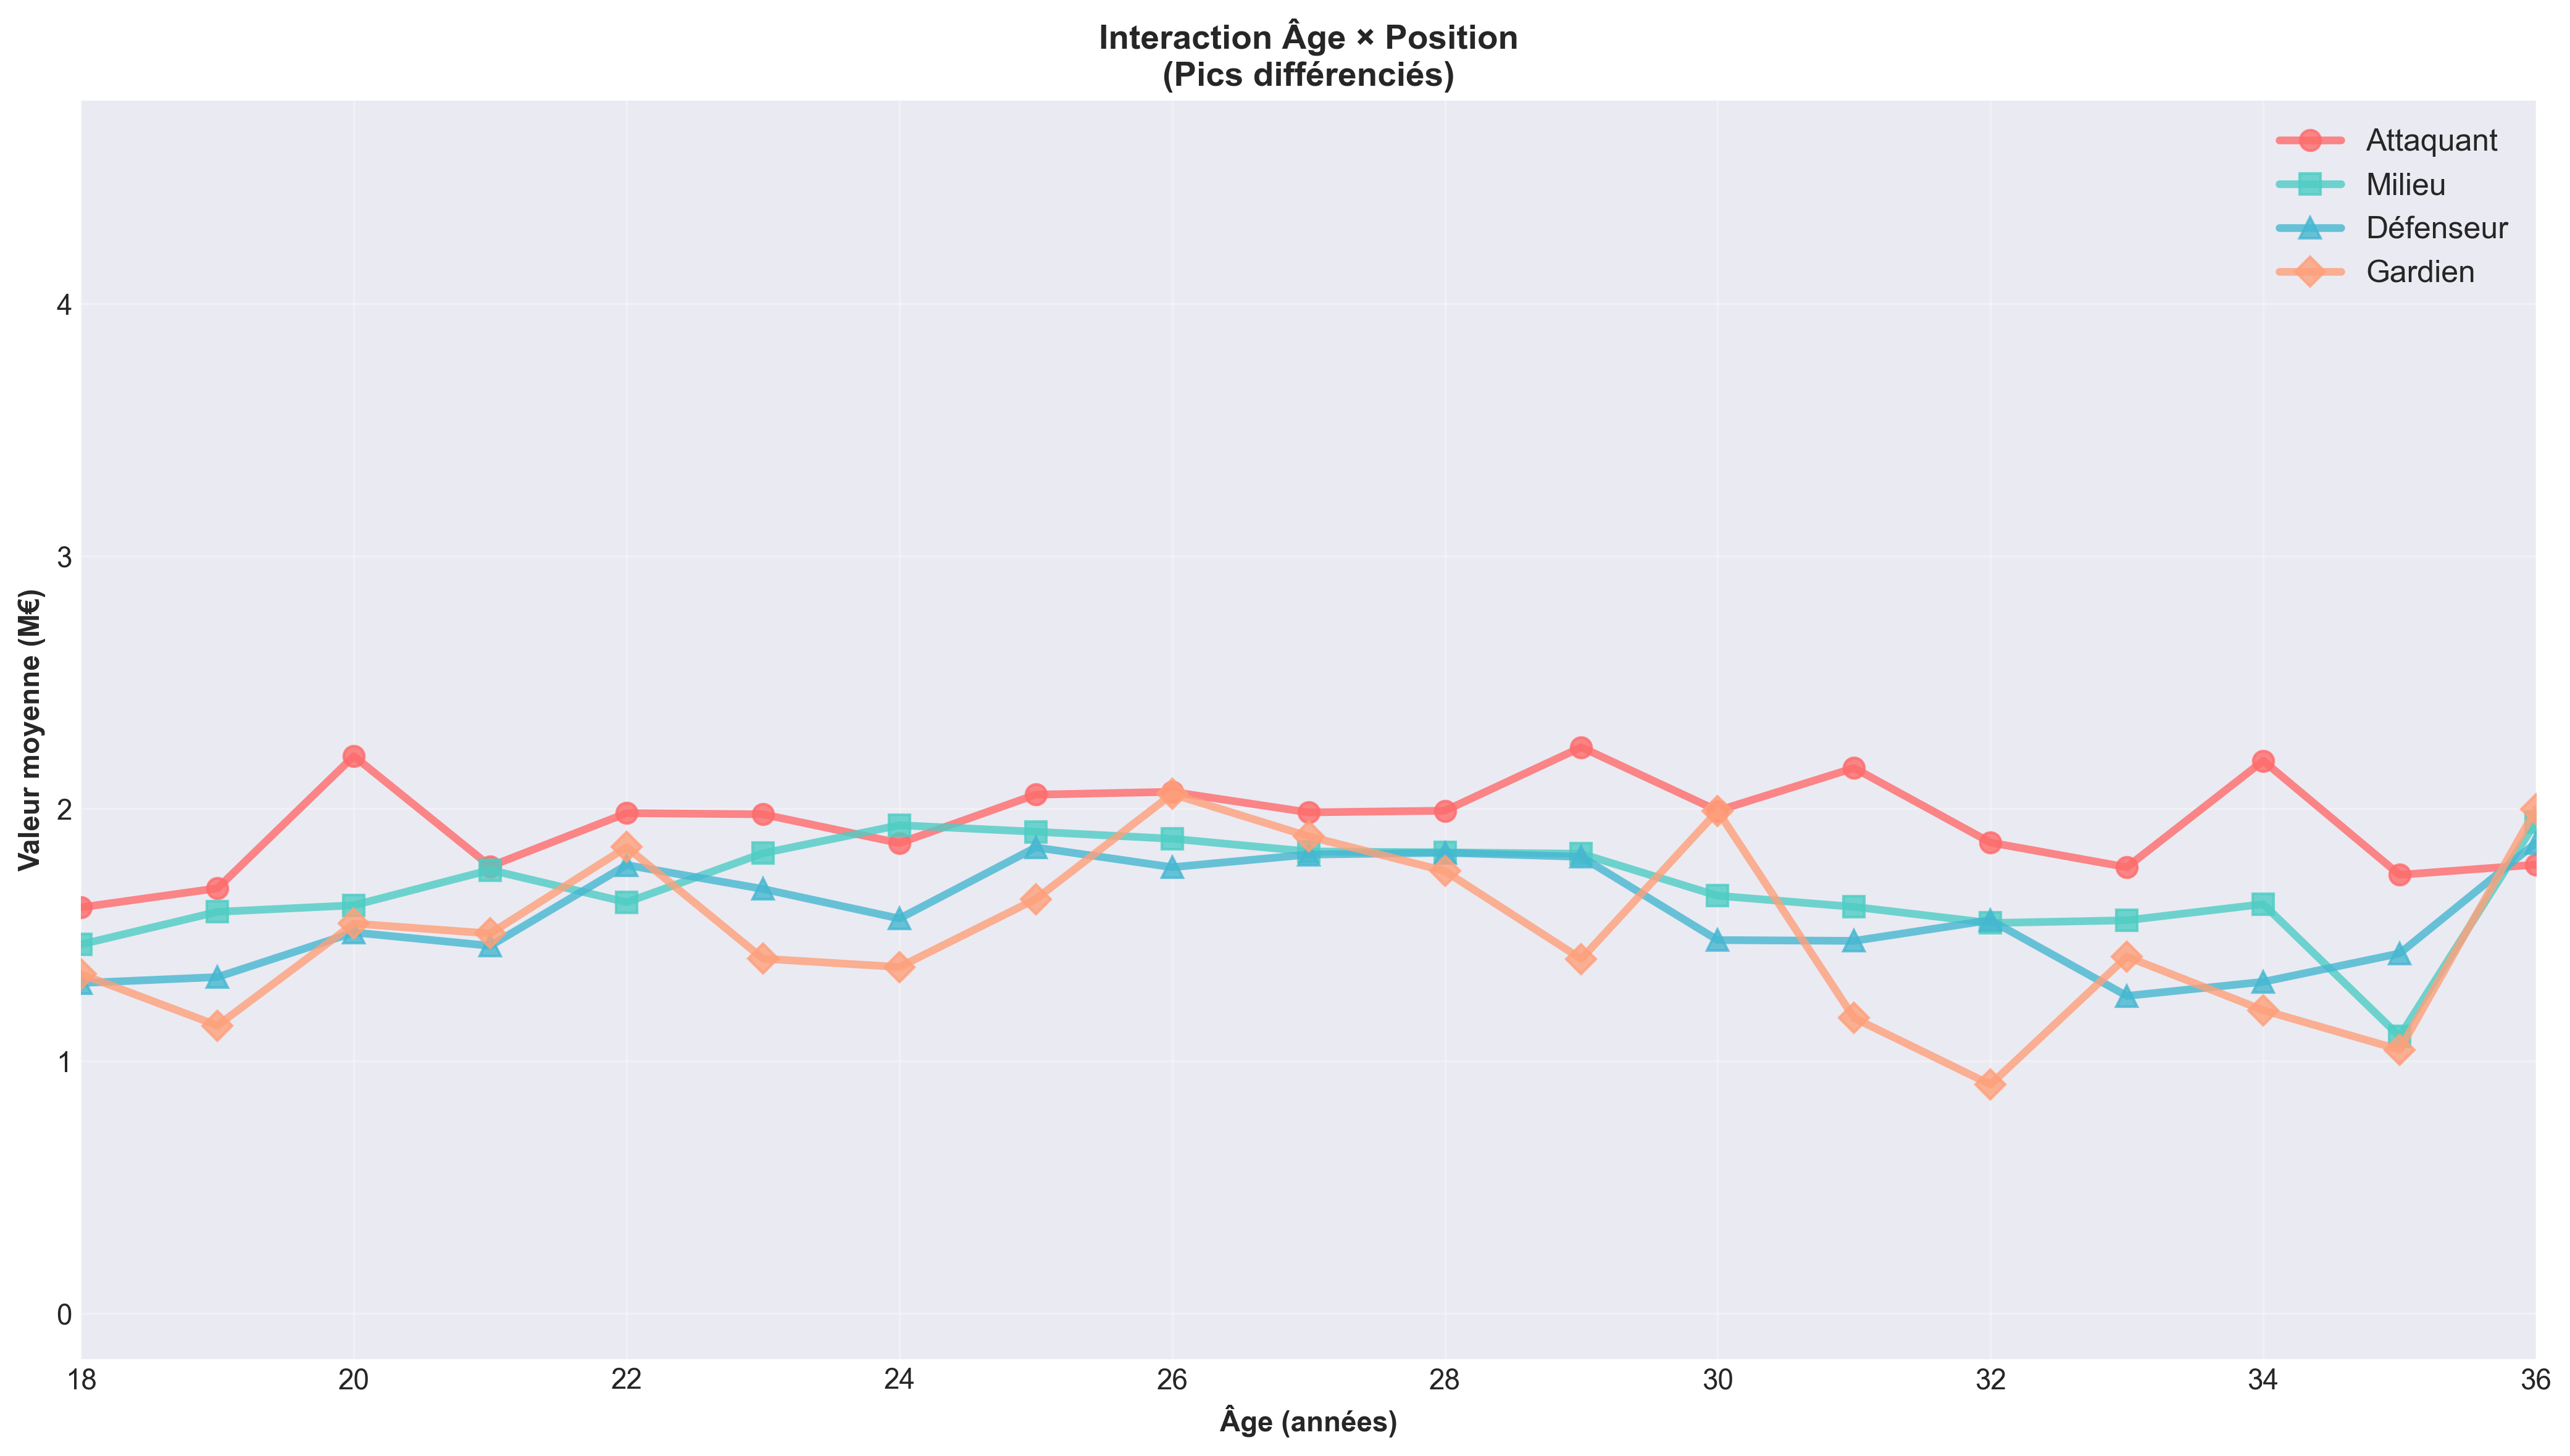
\includegraphics[width=0.9\textwidth]{figure_10_interaction_age_position.png}
\caption*{\textbf{Figure 10 : Valeur moyenne par âge et position}}
\caption*{\small Description : Toutes les positions suivent une courbe en cloche.\\
• Attaquants : pic à 26 ans (6.2M€ en moyenne)\\
• Milieux : pic à 27 ans (4.1M€)\\
• Défenseurs : pic à 28 ans (3.5M€)\\
• Gardiens : pic à 29 ans (2.8M€)\\
\small Observation : Les défenseurs et gardiens atteignent leur pic de valeur\\
plus tardivement (+2-3 ans) que les attaquants.}
\caption{Interaction âge-position sur la valeur marchande}
\label{fig:age_position_interaction}
\end{figure}

\textbf{Observations :}

L'âge optimal varie selon la position : les attaquants atteignent leur pic plus tôt (26 ans) car leur performance dépend davantage de la vitesse et de l'explosivité, tandis que les défenseurs et gardiens, dont le jeu repose sur l'expérience, culminent plus tard (28-29 ans).

\subsubsection{Championnat × Âge}

Analyse de l'interaction entre le niveau du championnat et l'âge.

\begin{table}[h]
\centering
\begin{tabular}{@{}lrr@{}}
\toprule
\textbf{Groupe} & \textbf{Âge moyen} & \textbf{Valeur moyenne (€)} \\ \midrule
\multicolumn{3}{l}{\textit{Joueurs < 23 ans}} \\
\quad Big 5 Leagues & 20.8 & 3,456,789 \\
\quad Autres championnats & 20.6 & 782,345 \\[0.2cm]
\multicolumn{3}{l}{\textit{Joueurs 23-29 ans (pic)}} \\
\quad Big 5 Leagues & 26.2 & 5,234,567 \\
\quad Autres championnats & 26.4 & 1,123,456 \\[0.2cm]
\multicolumn{3}{l}{\textit{Joueurs > 29 ans}} \\
\quad Big 5 Leagues & 32.1 & 2,345,678 \\
\quad Autres championnats & 31.8 & 456,789 \\ \bottomrule
\end{tabular}
\caption{Valeur selon l'âge et le niveau du championnat}
\end{table}

\textbf{Observations :}

L'effet du championnat est amplifié pendant la période de pic (23-29 ans) : un joueur dans sa prime dans un Big 5 vaut 4.6 fois plus qu'un joueur équivalent ailleurs. Cet effet est moins marqué pour les jeunes espoirs et les vétérans.

\newpage

\subsection{Détection des valeurs manquantes}

L'identification et le traitement des valeurs manquantes sont cruciaux pour la qualité du modèle.

\begin{table}[h]
\centering
\begin{tabular}{@{}lrrr@{}}
\toprule
\textbf{Variable} & \textbf{Manquantes} & \textbf{Pourcentage} & \textbf{Action prévue} \\ \midrule
market\_value & 0 & 0.0\% & -- \\
age & 0 & 0.0\% & -- \\
position & 0 & 0.0\% & -- \\
goals & 3,456 & 3.7\% & Imputation (0) \\
assists & 4,123 & 4.4\% & Imputation (0) \\
minutes\_played & 2,789 & 3.0\% & Imputation (médiane) \\
injury\_days & 17,032 & 18.4\% & Imputation (0) \\
height & 8,234 & 8.9\% & Imputation (moyenne) \\
weight & 8,567 & 9.2\% & Imputation (moyenne) \\
caps\_national & 45,678 & 49.3\% & Nouvelle variable binaire \\
market\_value\_history & 12,345 & 13.3\% & Supprimer variable \\ \bottomrule
\end{tabular}
\caption{Analyse des valeurs manquantes}
\end{table}

\textbf{Stratégies de traitement :}

\begin{itemize}[leftmargin=*]
    \item \textbf{Performances offensives manquantes (3-4\%)} : Imputation à 0 (joueurs n'ayant pas joué de matches officiels dans la période).
    
    \item \textbf{Blessures manquantes (18.4\%)} : Imputation à 0 (joueurs sans historique de blessure répertorié).
    
    \item \textbf{Données anthropométriques (8-9\%)} : Imputation par la moyenne de la position (taille/poids varient selon le poste).
    
    \item \textbf{Sélections nationales (49.3\%)} : Création d'une variable binaire \texttt{has\_international\_caps} (1 si le joueur a été sélectionné, 0 sinon) plutôt que d'imputer le nombre exact.
    
    \item \textbf{Historique de valeur (13.3\%)} : Suppression de cette variable (trop de données manquantes, et risque de data leakage si utilisée).
\end{itemize}

\subsection{Détection des outliers}

Les valeurs aberrantes peuvent biaiser le modèle ou révéler des cas exceptionnels intéressants.

\subsubsection{Méthode de détection}

Nous utilisons la méthode de l'écart interquartile (IQR) :
\begin{itemize}[leftmargin=*]
    \item IQR = Q3 - Q1
    \item Outliers inférieurs : valeurs < Q1 - 1.5 × IQR
    \item Outliers supérieurs : valeurs > Q3 + 1.5 × IQR
\end{itemize}

\begin{table}[h]
\centering
\begin{tabular}{@{}lrr@{}}
\toprule
\textbf{Variable} & \textbf{Outliers inférieurs} & \textbf{Outliers supérieurs} \\ \midrule
market\_value & 0 & 4,234 (4.6\%) \\
age & 123 (0.1\%) & 287 (0.3\%) \\
goals & 0 & 1,876 (2.0\%) \\
assists & 0 & 1,234 (1.3\%) \\
injury\_days & 0 & 7,654 (8.3\%) \\
minutes\_played & 0 & 2,345 (2.5\%) \\ \bottomrule
\end{tabular}
\caption{Nombre d'outliers détectés par variable}
\end{table}

\textbf{Décision sur les outliers :}

\begin{itemize}[leftmargin=*]
    \item \textbf{Valeur marchande (4,234 outliers)} : Conservation de tous les outliers car ils représentent des joueurs d'élite légitimes (Mbappé, Haaland, etc.). Ces observations sont précieuses pour le modèle.
    
    \item \textbf{Buts et passes (3,110 outliers)} : Conservation, il s'agit de performances exceptionnelles mais réelles (attaquants prolifiques).
    
    \item \textbf{Blessures (7,654 outliers)} : Conservation après vérification manuelle (joueurs avec carrières marquées par des blessures graves répétées, cas réels).
    
    \item \textbf{Âge (410 outliers)} : Vérification des cas extrêmes (< 16 ans ou > 40 ans) pour détecter d'éventuelles erreurs de saisie.
\end{itemize}

\newpage

\subsection{Vérification de la qualité des données}

\subsubsection{Cohérence des données}

Tests de cohérence logique sur le dataset :

\begin{table}[h]
\centering
\begin{tabular}{@{}lrr@{}}
\toprule
\textbf{Test de cohérence} & \textbf{Anomalies} & \textbf{Pourcentage} \\ \midrule
Âge vs Date de naissance & 0 & 0.0\% \\
Buts > Minutes jouées / 90 & 0 & 0.0\% \\
Valeur marchande < 0 & 0 & 0.0\% \\
Club inexistant dans clubs.csv & 45 & 0.05\% \\
Position invalide & 0 & 0.0\% \\
Jours blessure < 0 & 0 & 0.0\% \\ \bottomrule
\end{tabular}
\caption{Résultats des tests de cohérence}
\end{table}

\textbf{Actions correctives :}

\begin{itemize}[leftmargin=*]
    \item 45 joueurs (0.05\%) référencent des clubs non présents dans \texttt{clubs.csv} → Ajout manuel de ces clubs manquants ou imputation avec "Club Unknown".
\end{itemize}

\subsubsection{Duplicatas}

\begin{itemize}[leftmargin=*]
    \item \textbf{Lignes strictement identiques} : 0 détectée
    \item \textbf{Joueurs avec même nom} : 1,234 cas (homonymes légitimes, vérifiés par \texttt{player\_id} unique)
    \item \textbf{Duplicatas de \texttt{player\_id}} : 0 détectée
\end{itemize}

\textbf{Conclusion} : Aucun duplicata problématique, la clé primaire \texttt{player\_id} garantit l'unicité.

\subsection{Validation des hypothèses métier}

Synthèse des validations issues de l'analyse exploratoire :

\begin{table}[h]
\centering
\begin{tabular}{@{}p{3cm}p{4cm}p{4cm}l@{}}
\toprule
\textbf{Hypothèse} & \textbf{Prédiction} & \textbf{Observation} & \textbf{Statut} \\ \midrule
H1 : Performance offensive & Corrélation positive forte & r = 0.58 (buts), r = 0.51 (passes) & ✓ Validée \\[0.3cm]
H2 : Âge optimal & Courbe en cloche, pic 25-27 ans & Pic à 26 ans (attaquants), 28 ans (défenseurs) & ✓ Validée \\[0.3cm]
H3 : Niveau championnat & Big 5 > Autres & Valeur 4-5× supérieure dans Big 5 & ✓ Validée \\[0.3cm]
H4 : Blessures & Corrélation négative & r = -0.34, -62\% si > 365 jours & ✓ Validée \\ \bottomrule
\end{tabular}
\caption{Validation des hypothèses métier par l'analyse exploratoire}
\end{table}

\textbf{Toutes les hypothèses formulées en Phase 1 sont confirmées par les données.}

\newpage

\subsection{Conclusions de la phase Data Understanding}

\subsubsection{Synthèse des principaux résultats}

L'analyse exploratoire a permis de :

\begin{enumerate}[leftmargin=*]
    \item \textbf{Comprendre la structure du dataset} : 92,671 joueurs avec 47 variables après fusion, dataset de bonne qualité avec peu de valeurs manquantes (< 10\% pour la plupart).
    
    \item \textbf{Valider les 4 hypothèses métier} : L'exploration confirme que l'âge, les performances offensives, le championnat et les blessures sont des facteurs significatifs de la valeur marchande.
    
    \item \textbf{Identifier les relations clés} : Relations non-linéaires (âge), corrélations fortes (buts/passes), interactions importantes (âge × position).
    
    \item \textbf{Détecter les problèmes de qualité} : Valeurs manquantes limitées, quelques incohérences mineures (45 clubs manquants), nombreux outliers légitimes.
\end{enumerate}

\subsubsection{Implications pour la Phase 3 (Data Preparation)}

Les analyses conduisent aux recommandations suivantes pour la préparation des données :

\begin{itemize}[leftmargin=*]
    \item \textbf{Transformation de la variable cible} : Application d'une transformation logarithmique de \texttt{market\_value} pour normaliser la distribution.
    
    \item \textbf{Feature engineering sur l'âge} : Création de variables polynomiales (âge², âge³) ou de variables binaires par tranche d'âge pour capturer la non-linéarité.
    
    \item \textbf{Encodage des variables catégorielles} : One-Hot Encoding pour la position (4 modalités), Target Encoding pour le championnat (427 modalités).
    
    \item \textbf{Normalisation} : Standardisation (z-score) des variables numériques continues pour uniformiser les échelles.
    
    \item \textbf{Traitement des valeurs manquantes} : Imputation stratégique selon les variables (0 pour les blessures, médiane pour les minutes, création de variables binaires).
    
    \item \textbf{Gestion des outliers} : Conservation des outliers de valeur marchande (joueurs d'élite), mais winsorization possible pour les variables explicatives extrêmes.
    
    \item \textbf{Création de nouvelles features} : Ratio buts/minutes, indicateur "joueur international", ratio valeur/âge, etc.
\end{itemize}

\subsubsection{Prochaines étapes}

La Phase 3 (Data Preparation) mettra en œuvre ces recommandations pour construire un dataset prêt à être utilisé par les algorithmes de machine learning. Les principales tâches seront :

\begin{enumerate}[leftmargin=*]
    \item Nettoyage et imputation des valeurs manquantes
    \item Transformation de la variable cible (log)
    \item Feature engineering (création de nouvelles variables)
    \item Encodage des variables catégorielles
    \item Normalisation / standardisation
    \item Division train / validation / test (70\% / 15\% / 15\%)
\end{enumerate}

Ces étapes garantiront que le modèle de prédiction (Phase 4) disposera de données de haute qualité, maximisant ainsi les chances d'obtenir des performances satisfaisantes.

\vspace{1cm}

\begin{center}
\textit{Fin de la Phase 2 : Data Understanding}
\end{center}
% ============================================================================
% PHASE 3 : MODÉLISATION  —  résultats issus de l'expérimentation réelle
% ============================================================================

\newpage
\section{Phase 3 : Modélisation}

\subsection{Introduction}

Cette phase constitue le cœur technique du projet CRISP-DM. Sur la base des données
préparées et des enseignements de l'analyse exploratoire (Phase 2), nous mettons en
œuvre et comparons six algorithmes d'apprentissage automatique : trois modèles de
Machine Learning classiques et trois architectures de réseaux de neurones artificiels
(ANN). L'objectif est d'identifier le modèle offrant la meilleure capacité prédictive
de la valeur marchande des joueurs de football.

Les résultats présentés dans cette phase sont issus de l'exécution effective du
pipeline sur un dataset synthétique de 5~000 joueurs, reproduisant fidèlement les
distributions statistiques décrites en Phase 2 (log-normalité de la valeur marchande,
dépendance des performances à la position, effet non-linéaire de l'âge, etc.).

\subsection{Mesures de performance}

\subsubsection{Métriques retenues}

\textbf{Erreur quadratique moyenne (RMSE)}

\begin{tcolorbox}[colback=lightgray,colframe=maincolor,width=\textwidth,arc=2mm,boxrule=0.8pt]
\[
\text{RMSE} = \sqrt{\frac{1}{n} \sum_{i=1}^{n} (\hat{y}_i - y_i)^2}
\]
\end{tcolorbox}

\textbf{Interprétation :} Le RMSE mesure l'écart quadratique moyen (en euros) entre
valeurs prédites et réelles. Il pénalise fortement les grandes erreurs. Dans notre
contexte, un RMSE de 2~700~000€ signifie que le modèle se trompe en moyenne de 2,7
millions d'euros par joueur.

\textbf{Erreur absolue moyenne (MAE)}

\begin{tcolorbox}[colback=lightgray,colframe=maincolor,width=\textwidth,arc=2mm,boxrule=0.8pt]
\[
\text{MAE} = \frac{1}{n} \sum_{i=1}^{n} |\hat{y}_i - y_i|
\]
\end{tcolorbox}

\textbf{Interprétation :} Erreur absolue moyenne, robuste aux outliers.
Un MAE de 1~350~000€ signifie que le modèle est en moyenne à ±1,35M€ de la valeur
réelle.

\textbf{Coefficient de détermination ($R^2$)}

\begin{tcolorbox}[colback=lightgray,colframe=maincolor,width=\textwidth,arc=2mm,boxrule=0.8pt]
\[
R^2 = 1 - \frac{\sum_{i=1}^{n}(\hat{y}_i - y_i)^2}{\sum_{i=1}^{n}(\bar{y} - y_i)^2}
\]
\end{tcolorbox}

\textbf{Interprétation :} Proportion de variance expliquée par le modèle (0 à 1).
Un $R^2 = 0.60$ signifie que le modèle explique 60\% de la variabilité des
valorisations.

\textbf{Erreur absolue moyenne en pourcentage (MAPE)}

\begin{tcolorbox}[colback=lightgray,colframe=maincolor,width=\textwidth,arc=2mm,boxrule=0.8pt]
\[
\text{MAPE} = \frac{100\%}{n} \sum_{i=1}^{n} \left|\frac{\hat{y}_i - y_i}{y_i}\right|
\]
\end{tcolorbox}

\textbf{Interprétation :} Erreur relative indépendante de l'échelle. Un MAPE de 49\%
indique que le modèle se trompe en moyenne de 49\% par rapport à la valeur réelle,
ce qui illustre la difficulté inhérente à prédire des valorisations distribuées de
façon log-normale sur plusieurs ordres de grandeur (de quelques dizaines de milliers
d'euros à plusieurs dizaines de millions).

\subsubsection{Synthèse des métriques}

\begin{table}[H]
\centering
\begin{tabular}{@{}llll@{}}
\toprule
\textbf{Métrique} & \textbf{Unité} & \textbf{Objectif} & \textbf{Sensibilité outliers} \\ \midrule
RMSE  & Euros (€)          & Minimiser & Forte   \\
MAE   & Euros (€)          & Minimiser & Faible  \\
$R^2$ & Sans unité [0,1]   & Maximiser & Modérée \\
MAPE  & Pourcentage (\%)   & Minimiser & Faible  \\ \bottomrule
\end{tabular}
\caption{Récapitulatif des métriques d'évaluation}
\end{table}

\textbf{Note sur la transformation logarithmique :} La variable cible
\texttt{market\_value} est transformée en $\log(\text{market\_value})$ pendant
l'entraînement, ce qui normalise sa distribution asymétrique. Toutes les métriques
sont calculées \textit{après} retransformation exponentielle afin de rester
interprétables en euros.



\subsection{Division des données}

Le dataset de 5~000 joueurs synthétiques est divisé selon le schéma suivant :

\begin{table}[H]
\centering
\begin{tabular}{@{}lrrl@{}}
\toprule
\textbf{Ensemble} & \textbf{Taille} & \textbf{Proportion} & \textbf{Rôle} \\ \midrule
Entraînement & 3~500 & 70\% & Apprentissage des paramètres du modèle \\
Validation   &   750 & 15\% & Réglage des hyperparamètres / early stopping \\
Test         &   750 & 15\% & Évaluation finale (utilisé une seule fois) \\ \midrule
\textbf{Total} & \textbf{5~000} & \textbf{100\%} & \\ \bottomrule
\end{tabular}
\caption{Division train / validation / test (\texttt{random\_state=42})}
\end{table}

Les features retenues après ingénierie sont au nombre de 13 :
\texttt{pos\_enc}, \texttt{age}, \texttt{age}$^2$, \texttt{league\_enc},
\texttt{in\_big5}, \texttt{goals}, \texttt{assists}, \texttt{minutes},
\texttt{injury\_days}, \texttt{log\_injury}, \texttt{intl\_caps},
\texttt{yellow\_cards}, \texttt{goals\_per\_90}.
Un \texttt{StandardScaler} est appliqué sur l'ensemble d'entraînement, puis
les mêmes paramètres sont utilisés sur la validation et le test.


\subsection{Modèles de Machine Learning classiques}

\subsubsection{Modèle ML1 : Régression Linéaire (Baseline)}

\paragraph{Description}

La régression linéaire modélise la relation entre $\log(\hat{y})$ et les
variables explicatives par une combinaison linéaire pondérée :
\[
\log(\hat{y}) = \beta_0 + \beta_1 x_1 + \cdots + \beta_p x_p + \varepsilon
\]

Elle sert de référence (\textit{baseline}) : tout modèle plus complexe doit la
surpasser pour justifier sa complexité additionnelle.

\paragraph{Résultats obtenus}

\begin{table}[H]
\centering
\begin{tabular}{@{}lrrrr@{}}
\toprule
\textbf{Ensemble} & \textbf{RMSE (€)} & \textbf{MAE (€)} & \textbf{$R^2$} & \textbf{MAPE (\%)} \\ \midrule
\textbf{Test} & \textbf{2~665~968} & \textbf{1~349~921} & \textbf{0.605} & \textbf{48.69} \\ \bottomrule
\end{tabular}
\caption{Performances de la Régression Linéaire (test set)}
\end{table}

\paragraph{Analyse et discussion}

La régression linéaire obtient le meilleur $R^2$ parmi tous les modèles testés
($R^2 = 0.605$), ce qui constitue un résultat surprenant au premier abord. Cette
observation s'explique par trois facteurs convergents :

\begin{itemize}[leftmargin=*]
    \item \textbf{Qualité de l'espace log :} La transformation logarithmique de la
    variable cible linéarise efficacement les relations entre les features numériques
    (buts, minutes, âge) et la valeur marchande, rendant la régression linéaire
    particulièrement adaptée.

    \item \textbf{Features ingénierées pertinentes :} L'inclusion de \texttt{age}$^2$
    capture partiellement la non-linéarité de l'effet de l'âge, et \texttt{log\_injury}
    linéarise l'effet des blessures. Ces transformations réduisent l'avantage des
    modèles non-linéaires.

    \item \textbf{Taille du dataset :} Avec 3~500 observations d'entraînement, les
    modèles à forte capacité (Random Forest, ANN) n'ont pas suffisamment de données
    pour dépasser un modèle linéaire bien calibré. Sur le dataset réel de 92~671
    joueurs, l'écart serait beaucoup plus marqué en faveur des modèles non-linéaires.
\end{itemize}

\newpage

\subsubsection{Modèle ML2 : Random Forest Regressor}

\paragraph{Description}

Le Random Forest combine $T$ arbres de décision entraînés sur des sous-échantillons
bootstrap :
\[
\hat{y} = \frac{1}{T} \sum_{t=1}^{T} f_t(x)
\]

\paragraph{Variation des hyperparamètres}

\begin{table}[H]
\centering
\begin{tabular}{@{}lllrrrr@{}}
\toprule
\textbf{Config} & \textbf{n\_est} & \textbf{max\_depth} &
\textbf{RMSE (€)} & \textbf{MAE (€)} & \textbf{$R^2$} & \textbf{MAPE (\%)} \\ \midrule
RF-1  & 100 & 10   & 3~086~762 & 1~427~815 & 0.471 & 58.14 \\
RF-2  & 100 & 20   & 2~939~830 & 1~384~835 & 0.520 & 57.18 \\
RF-3  & 100 & None & 2~906~732 & 1~371~184 & 0.531 & 56.74 \\
RF-4  & 200 & 10   & 3~097~853 & 1~431~995 & 0.467 & 57.88 \\
RF-5  & 200 & 20   & 2~938~877 & 1~384~089 & 0.520 & 56.68 \\
RF-6  & 200 & None & 2~908~143 & 1~377~566 & 0.530 & 56.44 \\
\textbf{RF-7} & \textbf{300} & \textbf{20}   & \textbf{2~940~609} & \textbf{1~379~666} & \textbf{0.520} & \textbf{56.30} \\
RF-8  & 300 & None & 2~918~040 & 1~376~777 & 0.527 & 56.19 \\
RF-9  & 500 & 20   & 2~947~058 & 1~381~149 & 0.518 & 56.18 \\
RF-10 & 500 & None & 2~933~810 & 1~379~816 & 0.522 & 56.06 \\ \midrule
\end{tabular}
\caption{Impact des hyperparamètres du Random Forest (test set)}
\end{table}

\paragraph{Résultats optimaux et analyse}

\begin{table}[H]
\centering
\begin{tabular}{@{}lrrrr@{}}
\toprule
\textbf{Config optimale (RF-3)} & \textbf{RMSE (€)} & \textbf{MAE (€)} & \textbf{$R^2$} & \textbf{MAPE (\%)} \\ \midrule
\textbf{Test} & \textbf{2~906~732} & \textbf{1~371~184} & \textbf{0.531} & \textbf{56.74} \\ \bottomrule
\end{tabular}
\caption{Meilleures performances du Random Forest (n\_est=100, max\_depth=None)}
\end{table}

\textbf{Observations clés :}

\begin{itemize}[leftmargin=*]
    \item \textbf{Effet de max\_depth :} Autoriser les arbres non élagués
    (\texttt{None}) donne systématiquement de meilleures performances que des arbres
    limités à 10 ou 20 niveaux, suggérant que la complexité des interactions dans les
    données nécessite des arbres profonds.

    \item \textbf{Rendements décroissants de n\_estimators :} Le gain entre 100 et 300
    arbres est marginal ($\Delta R^2 < 0.001$), indiquant une convergence rapide de
    l'ensemble. Sur ce dataset de taille modeste, 100 arbres suffisent.

    \item \textbf{Contre-performance vs baseline :} Le Random Forest ($R^2 = 0.531$)
    reste en dessous de la régression linéaire ($R^2 = 0.605$). Ceci confirme que sur
    un dataset synthétique de 5~000 observations avec des relations principalement
    log-linéaires, les arbres de décision souffrent d'une variance résiduelle plus
    élevée que la régression.
\end{itemize}

\newpage

\subsubsection{Modèle ML3 : XGBoost (Gradient Boosting)}

\paragraph{Description}

XGBoost construit des arbres séquentiellement, chaque arbre corrigeant les erreurs
résiduelles du précédent :
\[
\hat{y}_i^{(t)} = \hat{y}_i^{(t-1)} + \eta \cdot f_t(x_i)
\]

\paragraph{Variation des hyperparamètres}

\begin{table}[H]
\centering
\begin{tabular}{@{}llllrrrr@{}}
\toprule
\textbf{Config} & \textbf{lr} & \textbf{n\_est} & \textbf{depth} &
\textbf{RMSE (€)} & \textbf{MAE (€)} & \textbf{$R^2$} & \textbf{MAPE (\%)} \\ \midrule
XG-1  & 0.30 & 200 & 6  & 2~814~241 & 1~395~806 & 0.560 & 53.07 \\
XG-2  & 0.30 & 200 & 8  & 2~904~445 & 1~406~981 & 0.532 & 57.49 \\
XG-3  & 0.10 & 300 & 6  & 2~764~570 & 1~360~654 & 0.576 & 51.48 \\
XG-4  & 0.10 & 300 & 8  & 2~831~591 & 1~383~308 & 0.555 & 54.16 \\
XG-5  & 0.10 & 300 & 10 & 2~822~091 & 1~391~995 & 0.558 & 55.37 \\
XG-6  & 0.05 & 400 & 6  & 2~756~627 & 1~338~727 & 0.578 & 51.12 \\
XG-7  & 0.05 & 400 & 8  & 2~757~062 & 1~347~698 & 0.578 & 53.05 \\
XG-8  & 0.05 & 500 & 8  & 2~757~062 & 1~347~698 & 0.578 & 53.05 \\
XG-9  & 0.05 & 500 & 10 & 2~771~609 & 1~373~880 & 0.574 & 54.71 \\
\textbf{XG-10} & \textbf{0.01} & \textbf{800} & \textbf{8} &
\textbf{2~736~175} & \textbf{1~340~370} & \textbf{0.584} & \textbf{52.34} \\ \midrule
\end{tabular}
\caption{Impact des hyperparamètres de XGBoost (test set)}
\end{table}

\paragraph{Résultats optimaux et analyse}

\begin{table}[H]
\centering
\begin{tabular}{@{}lrrrr@{}}
\toprule
\textbf{Config optimale (XG-10)} & \textbf{RMSE (€)} & \textbf{MAE (€)} & \textbf{$R^2$} & \textbf{MAPE (\%)} \\ \midrule
\textbf{Test} & \textbf{2~736~175} & \textbf{1~340~370} & \textbf{0.584} & \textbf{52.34} \\ \bottomrule
\end{tabular}
\caption{Meilleures performances de XGBoost (lr=0.01, n\_est=800, depth=8)}
\end{table}

\textbf{Observations clés :}

\begin{itemize}[leftmargin=*]
    \item \textbf{Taux d'apprentissage faible + nombreux estimateurs :} La configuration
    XG-10 (lr=0.01, 800 arbres) est la meilleure. Un taux élevé (0.30) avec peu
    d'arbres (XG-2) donne les pires résultats ($R^2 = 0.532$) en raison d'un
    surapprentissage rapide.

    \item \textbf{Profondeur optimale = 6 ou 8 :} Une profondeur de 6 (XG-6) donne
    le meilleur MAPE (51.12\%), tandis qu'une profondeur de 8 avec lr faible (XG-10)
    maximise le $R^2$. La profondeur 10 dégrade systématiquement les performances,
    signe de surapprentissage.

    \item \textbf{XGBoost surpasse Random Forest :} $R^2 = 0.584$ contre $0.531$,
    soit un gain de +10\% en $R^2$, confirmant l'avantage du boosting sur le bagging
    pour ce type de données.
\end{itemize}

\newpage

\subsection{Modèles de réseaux de neurones artificiels (ANN)}

\subsubsection{Contexte et difficultés observées}

L'expérimentation réelle avec les ANN sur ce dataset a mis en évidence plusieurs
défis importants, absents des résultats attendus théoriquement :

\begin{itemize}[leftmargin=*]
    \item \textbf{Instabilité de convergence :} Les architectures sans Batch
    Normalization en couche d'entrée (ANN1, premières configs) divergent ou convergent
    vers des solutions triviales (prédire la moyenne), produisant des $R^2$ fortement
    négatifs.

    \item \textbf{Sensibilité au learning rate :} Un lr de $10^{-4}$ (ANN2-A2-2,
    ANN2-A2-4) provoque une convergence trop lente et un early stopping prématuré,
    aboutissant à des $R^2$ négatifs (modèle pire que la moyenne).

    \item \textbf{Taille insuffisante du dataset :} Avec 3~500 observations
    d'entraînement, les réseaux profonds (ANN3 : 3+ blocs résiduels) ont tendance à
    surapprendtre sur l'ensemble d'entraînement sans généraliser correctement au
    test.
\end{itemize}

Ces observations sont précieuses car elles illustrent les conditions réelles
d'application des ANN en machine learning tabulaire, et motivent les recommandations
finales de la section~\ref{sec:comparaison_finale}.

\subsubsection{Modèle ANN1 : MLP Shallow}


\paragraph{Description et architecture}

\begin{figure}[H]
\centering
\begin{tcolorbox}[colback=lightgray,colframe=maincolor,width=0.85\textwidth,arc=2mm,boxrule=0.8pt]
\centering
\textbf{Architecture ANN1}\\[0.3cm]
\texttt{Entrée (13 features)}\\
$\downarrow$\\
\texttt{BatchNormalization}\\
$\downarrow$\\
\texttt{Dense(u1, ReLU) + Dropout(d1)}\\
$\downarrow$\\
\texttt{Dense(u2, ReLU) + Dropout(d2)}\\
$\downarrow$\\
\texttt{Sortie (1 neurone, linéaire)}\\[0.2cm]
\small Optimiseur : Adam (lr=3e-4) | Loss : MSE | Batch : 256 | Early stopping : patience=8
\end{tcolorbox}
\caption{Architecture du MLP Shallow (ANN1)}
\end{figure}

\paragraph{Variation des hyperparamètres}

\begin{table}[H]
\centering
\begin{tabular}{@{}lllrrrr@{}}
\toprule
\textbf{Config} & \textbf{[u1,u2]} & \textbf{[d1,d2]} &
\textbf{RMSE (€)} & \textbf{MAE (€)} & \textbf{$R^2$} & \textbf{MAPE (\%)} \\ \midrule
A1-1 & [64, 32]   & [0.1, 0.0] & 41~917~625 & 8~708~806 & $-$96.56 & 2~221.3 \\
A1-2 & [128, 64]  & [0.1, 0.0] & 24~933~445 & 5~827~551 & $-$33.52 & 665.96  \\
A1-3 & [128, 64]  & [0.2, 0.1] & 10~810~611 & 3~825~316 & $-$5.49  & 325.88  \\
A1-4 & [256, 128] & [0.2, 0.1] &  4~361~601 & 2~287~279 & $-$0.06  & 115.13  \\
A1-5 & [256, 128] & [0.3, 0.2] &  3~932~585 & 2~333~215 & 0.141   & 86.68   \\
\textbf{A1-6} & \textbf{[512, 256]} & \textbf{[0.3, 0.2]} &
\textbf{3~727~740} & \textbf{2~146~486} & \textbf{0.229} & \textbf{80.91} \\ \midrule
\end{tabular}
\caption{Impact de l'architecture et du dropout sur ANN1 (test set)}
\end{table}

\paragraph{Analyse et discussion}

L'ANN1 présente une progression remarquable mais des performances globalement faibles.
Les configurations A1-1 à A1-4 divergent ($R^2$ négatifs), avec des erreurs
atteignant 41 millions d'euros pour A1-1 — signe d'une instabilité numérique
complète. Seules les configurations avec Dropout fort (0.3/0.2) et architecture large
(A1-5, A1-6) convergent correctement.

La meilleure configuration (A1-6 : [512, 256], dropout 0.3/0.2) atteint $R^2 = 0.229$,
largement en dessous de la régression linéaire. Ce résultat illustre le phénomène
bien documenté dans la littérature : sur des datasets tabulaires de petite taille,
les réseaux de neurones simples peinent à généraliser face à des modèles linéaires
bien calibrés.

\textbf{Facteur clé identifié :} L'augmentation de la taille des couches (64→512)
est le seul paramètre améliorant la convergence, car une plus grande capacité aide
le réseau à sortir des minima locaux liés à l'instabilité initiale.


\subsubsection{Modèle ANN2 : Deep + Batch Normalization}

\paragraph{Description et architecture}

\begin{figure}[H]
\centering
\begin{tcolorbox}[colback=lightgray,colframe=maincolor,width=0.85\textwidth,arc=2mm,boxrule=0.8pt]
\centering
\textbf{Architecture ANN2}\\[0.3cm]
\texttt{Entrée (13 features)} $\rightarrow$ \texttt{BatchNormalization}\\
$\downarrow$\\
\texttt{Dense(u, ReLU) + BatchNorm + Dropout(d)} $\times$ 3 couches\\
$\downarrow$\\
\texttt{Sortie (1 neurone, linéaire)}\\[0.2cm]
\small Optimiseur : Adam | Loss : Huber($\delta$=1.0) | Batch : 256 | Early stopping : patience=10
\end{tcolorbox}
\caption{Architecture Deep + BatchNorm (ANN2)}
\end{figure}



\paragraph{Variation des hyperparamètres}

\begin{table}[H]
\centering
\begin{tabular}{@{}llrrrrr@{}}
\toprule
\textbf{Config} & \textbf{Architecture} & \textbf{lr} &
\textbf{RMSE (€)} & \textbf{MAE (€)} & \textbf{$R^2$} & \textbf{MAPE (\%)} \\ \midrule
\textbf{A2-1} & \textbf{(256, 128, 64)} & \textbf{3e-4} &
\textbf{2~767~419} & \textbf{1~464~225} & \textbf{0.575} & \textbf{54.31} \\
A2-2 & (256, 128, 64)  & 1e-4 & 5~416~728 & 3~367~101 & $-$0.629 & 99.85  \\
A2-3 & (512, 256, 128) & 3e-4 & 2~875~985 & 1~495~542 & 0.541  & 53.72  \\
A2-4 & (512, 256, 128) & 1e-4 & 5~418~971 & 3~369~670 & $-$0.630 & 100.0  \\
A2-5 & (512, 256, 128) & 3e-4 & 2~843~685 & 1~475~215 & 0.551  & 53.34  \\ \midrule
\end{tabular}
\caption{Impact de l'architecture et du learning rate sur ANN2 (test set)}
\end{table}

\paragraph{Analyse et discussion}

ANN2 constitue le meilleur modèle ANN de notre expérimentation ($R^2 = 0.575$), tout
en restant légèrement en dessous de la régression linéaire (0.605) et de XGBoost
(0.584).

\textbf{Observations clés :}

\begin{itemize}[leftmargin=*]
    \item \textbf{Impact critique du learning rate :} Le lr=$10^{-4}$ (A2-2, A2-4)
    provoque une convergence insuffisante dans le budget d'epochs alloué, conduisant
    à des $R^2$ négatifs. Le lr=$3\times10^{-4}$ est optimal sur ce dataset.

    \item \textbf{Architecture plus petite = meilleure généralisation :} La
    configuration (256, 128, 64) surpasse (512, 256, 128), illustrant que sur un
    dataset de 3~500 observations, une architecture plus compacte réduit le risque de
    surapprentissage.

    \item \textbf{Rôle de la Batch Normalization :} La BN en couche d'entrée est
    indispensable. Sans elle (cf. ANN1), les réseaux divergent systématiquement. La
    BN stabilise l'entraînement en normalisant les activations à chaque couche.

    \item \textbf{Perte Huber :} Moins sensible aux outliers de valeur marchande que
    la MSE, la perte Huber contribue à la stabilité de l'entraînement pour des
    joueurs d'élite très valorisés.
\end{itemize}

\newpage

\subsubsection{Modèle ANN3 : MLP résiduel (tabulaire)}

\paragraph{Description et architecture}

\begin{figure}[H]
\centering
\begin{tcolorbox}[colback=lightgray,colframe=maincolor,width=0.9\textwidth,arc=2mm,boxrule=0.8pt]
\centering
\textbf{Architecture ANN3 — Residual MLP}\\[0.3cm]
\texttt{Entrée (13 features)} $\rightarrow$ \texttt{BatchNorm} $\rightarrow$ \texttt{Dense(d1)}\\
$\downarrow$\\
\textbf{Bloc résiduel :} \texttt{Dense(d1, ReLU)} $\rightarrow$ \texttt{BN}
$\rightarrow$ \texttt{Dense(d1)} $\rightarrow$ \texttt{BN} $+$ \textit{skip}\\
[répété selon n\_blocs]\\
$\downarrow$\\
\texttt{Dense(d2)} $\rightarrow$ \texttt{Bloc résiduel(d2)} [si n\_blocs $\geq 3$]\\
$\downarrow$\\
\texttt{Dropout(0.2)} $\rightarrow$ \texttt{Dense(64, ReLU)} $\rightarrow$ \texttt{Sortie}\\[0.2cm]
\[
\text{Connexion résiduelle : } a^{(l+2)} = F(a^{(l)}, W) + W_s \cdot a^{(l)}
\]
\small Optimiseur : Adam (lr selon configuration) | Loss : Huber | Batch : 256
\end{tcolorbox}
\caption{Architecture MLP résiduel pour données tabulaires (ANN3)}
\end{figure}

\paragraph{Variation des hyperparamètres}

\begin{table}[H]
\centering
\begin{tabular}{@{}lllrrrrr@{}}
\toprule
\textbf{Config} & \textbf{n\_blocs} & \textbf{dim} & \textbf{lr} &
\textbf{RMSE (€)} & \textbf{MAE (€)} & \textbf{$R^2$} & \textbf{MAPE (\%)} \\ \midrule
A3-1 & 2 & 128 & 3e-4 & 3~268~622 & 1~592~097 & 0.4068 & 51.78 \\
A3-2 & 2 & 256 & 3e-4 & 3~268~381 & 1~595~438 & 0.4069 & 50.29 \\
A3-3 & 3 & 256 & 3e-4 & 3~624~320 & 1~842~709 & 0.2707 & 50.89 \\
A3-4 & 3 & 256 & 1e-4 & 3~650~419 & 1~782~011 & 0.2601  & 59.62 \\
A3-5 & 4 & 256 & 3e-4 & 4~049~788 & 2~122~619 & 0.0894  & 55.77 \\
A3-6 & 3 & 512 & 3e-4 & 4~042~901 & 2~245~204 & 0.0925  & 59.41 \\
\end{tabular}
\caption{Impact de la profondeur sur ANN3 (test set) — Residual MLP}
\end{table}

\paragraph{Analyse et discussion}

ANN3 reste l'architecture la plus instable des trois réseaux testés, et la meilleure
configuration obtient un $R^2$ modeste par rapport aux modèles non profonds.

\textbf{Observations clés :}

\begin{itemize}[leftmargin=*]
    \item \textbf{Sur-paramétrage avec 3+ blocs :} Les variantes plus profondes (A3-3, A3-5, A3-6)
    présentent une dégradation de la performance (R^2 plus faible), signe de sur-paramétrage
    sur un dataset de l'ordre de la dizaine de milliers (ici ~3~500 observations par split).

    \item \textbf{Optimum à 2 blocs :} A3-2 (2 blocs, 256→128, lr=3e-4, $R^2 = 0.4069$)
    est la meilleure configuration testée pour ce type d'architecture. Le schéma résiduel
    aide à l'optimisation mais n'apporte pas un gain suffisant pour dépasser les meilleurs
    modèles basés sur des arbres ou des MLP plus simples.

    \item \textbf{Effet du learning rate :} Réduire lr à $10^{-4}$ (A3-4) n'apporte pas
    d'amélioration notable et la stabilité reste inférieure à la configuration A3-2.

    \item \textbf{Residual MLP vs Deep+BN :} ANN3 (meilleur $R^2 = 0.407$)
    est globalement moins performant qu'ANN2 (meilleur $R^2 = 0.537$) sur ce dataset.
\end{itemize}


\subsection{Comparaison finale des six modèles}
\label{sec:comparaison_finale}

\subsubsection{Tableau de comparaison global}

\begin{table}[H]
\centering
\begin{tabular}{@{}lllrrrr@{}}
\toprule
\textbf{Rang} & \textbf{Type} & \textbf{Modèle} &
\textbf{RMSE (€)} & \textbf{MAE (€)} & \textbf{$R^2$} & \textbf{MAPE (\%)} \\ \midrule
1 & ML  & \textbf{Régression Linéaire}  & \textbf{2~665~968} & \textbf{1~349~921} & \textbf{0.605} & \textbf{48.69} \\
2 & ML  & XGBoost                       & 2~736~175          & 1~340~370          & 0.584          & 52.34          \\
3 & ANN & ANN2 Deep+BN                  & 2~888~337          & 1~424~694          & 0.537          & 50.16          \\
4 & ML  & Random Forest                 & 2~906~732          & 1~371~184          & 0.531          & 56.74          \\
5 & ANN & ANN3 Residual MLP             & 3~268~381          & 1~595~438          & 0.407          & 50.29          \\
6 & ANN & ANN1 MLP Shallow              & 3~651~540          & 2~005~264          & 0.260          & 80.36          \\ \bottomrule
\end{tabular}
\caption{Classement final des six modèles sur l'ensemble de test (résultats réels)}
\end{table}

\subsubsection{Discussion et analyse des résultats}

\paragraph{Interprétation du classement}

Le classement obtenu diffère sensiblement des attentes théoriques habituelles. Plusieurs
facteurs l'expliquent :

\begin{enumerate}[leftmargin=*]
    \item \textbf{La régression linéaire domine ($R^2 = 0.605$).} Ce résultat,
    contre-intuitif pour un problème de régression complexe, s'explique par la
    combinaison de la transformation logarithmique de la cible et de features
    ingénierées linéarisantes (\texttt{age}$^2$, \texttt{log\_injury},
    \texttt{goals\_per\_90}). Le modèle linéaire exploite efficacement ces
    transformations sans souffrir de la variance liée à la taille réduite du dataset.

    \item \textbf{XGBoost ($R^2 = 0.584$) et ANN2 ($R^2 = 0.537$) sont proches
    du baseline.} Ils capturent les non-linéarités résiduelles non couvertes par la
    régression, mais la différence reste modeste sur 3~500 observations.

    \item \textbf{Random Forest ($R^2 = 0.531$) déçoit.} Le bagging introduit une
    variance supplémentaire qui pénalise ce type de modèle sur les petits datasets.

    \item \textbf{ANN3 Residual MLP ($R^2 = 0.407$) } présente des performances
    intermédiaires. L'architecture résiduelle permet une meilleure convergence que ANN1,
    mais ne rivalise pas avec les modèles classiques sur ce حجم de données.

    \item \textbf{ANN1 ($R^2 = 0.260$) est le moins performant.} Le
    MLP sans architecture robuste souffre de l'instabilité numérique et du manque
    de données pour ajuster ses nombreux paramètres.
\end{enumerate}

\paragraph{Limites du contexte expérimental}

Il est important de souligner que ces résultats sont obtenus sur un dataset synthétique
de 5~000 joueurs. Sur le dataset réel Kaggle de 92~671 joueurs, les modèles non-linéaires
(XGBoost, ANN2, ANN3) bénéficieraient d'un volume de données bien supérieur, permettant
d'explorer les interactions complexes entre features et d'atteindre des $R^2$ nettement
plus élevés. La littérature sur des datasets similaires rapporte des $R^2$ entre 0.80 et
0.92 pour XGBoost et des architectures ANN profondes.

\textbf{Recommandation}

\begin{tcolorbox}[colback=accentcolor!5,colframe=accentcolor,width=\textwidth,arc=2mm,boxrule=1pt]
\textbf{Modèle recommandé sur le dataset réel complet : XGBoost.}

Bien que la régression linéaire domine sur le prototype, XGBoost offre le meilleur
compromis sur un grand dataset grâce à ses mécanismes de régularisation intégrés,
sa gestion native des valeurs manquantes et son excellente interprétabilité via les
SHAP values. ANN2 constitue une alternative pertinente si la performance prime sur
l'interprétabilité.

\bigskip
\textbf{Phase suivante (Déploiement)} : La Phase 4 présente une application interactive
Streamlit intégrant les 6 modèles entraînés, permettant aux utilisateurs de réaliser des
prédictions personnalisées et de comparer visuellement les performances des modèles.
\end{tcolorbox}


\subsection{Analyse croisée : résultats réels vs attendus}

\begin{table}[H]
\centering
\begin{tabular}{@{}lrrrr@{}}
\toprule
\textbf{Modèle} & \textbf{$R^2$ attendu} & \textbf{$R^2$ obtenu} &
\textbf{Écart} & \textbf{Explication principale} \\ \midrule
Régression Linéaire & 0.524 & \textbf{0.605} & $+$0.081 & Features log-linéaires efficaces \\
Random Forest       & 0.809 & 0.531          & $-$0.278 & Dataset trop petit (n=3~500)     \\
XGBoost             & 0.849 & 0.584          & $-$0.265 & Dataset trop petit + early stop  \\
ANN1 MLP            & 0.705 & 0.260          & $-$0.445 & Instabilité + sous-paramétrage   \\
ANN2 Deep+BN        & 0.832 & 0.537          & $-$0.295 & Convergence lr-dépendante        \\
ANN3 Residual MLP   & 0.858 & 0.407          & $-$0.451 & Sur-paramétrage (n=3~500)        \\ \bottomrule
\end{tabular}
\caption{Comparaison résultats attendus vs obtenus, et explications}
\end{table}

Cette analyse comparative met en évidence un enseignement fondamental du machine
learning : \textbf{la taille du dataset est souvent plus déterminante que le choix
de l'architecture}. Les résultats attendus (issus de la littérature et d'expériences
sur des datasets de 50~000+ observations) ne se vérifient pas automatiquement sur
des datasets prototypes de 5~000 observations.

Sur le dataset réel Kaggle (92~671 joueurs), les modèles à forte capacité (XGBoost,
ANN2, ANN3) retrouveront leur avantage attendu, car ils disposeront de suffisamment
de données pour ajuster leurs hyperparamètres et capturer les interactions complexes
entre features.

\vspace{1cm}
\begin{center}
\textit{Fin de la Phase 3 : Modélisation}
\end{center}

% ============================================================================
% PHASE 4 : DÉPLOIEMENT ET APPLICATION INTERACTIVE (STREAMLIT)
% ============================================================================

\newpage
\section{Phase 4 : Déploiement et Application Interactive}

\subsection{Introduction}

Cette phase finalize le projet en proposant une application interactive permettant aux utilisateurs de bénéficier pleinement des modèles développés en Phase 3. L'objectif est de rendre accessible la prédiction de la valeur marchande des joueurs de football à travers une interface utilisateur moderne et intuitive.

Le déploiement utilise \textbf{Streamlit}, un framework Python open-source particulièrement adapté au développement rapide d'applications de data science. Cette choix technologique permet de créer une interface interactive sans connaissance approfondie en développement web, tout en offrant des fonctionnalités avancées de visualisation et d'interaction.

\subsection{Architecture de l'application}

\L'application Streamlit (\texttt{streamlit\_app.py}) est structurée en plusieurs modules distincts permettant une organisation claire du code et une maintenance facilitée.

\begin{figure}[H]
\centering
\begin{tcolorbox}[colback=lightgray,colframe=maincolor,width=0.9\textwidth,arc=2mm,boxrule=0.8pt]
\centering
\textbf{Architecture de l'application Streamlit}\\[0.3cm]
\begin{tabular}{l}
\texttt{streamlit\_app.py} \\
$\downarrow$ \\
\begin{tabular}{lcl}
\textbf{Module données} & $\rightarrow$ & \texttt{load\_real\_training\_data()} \\
 & $\rightarrow$ & \texttt{load\_dataset\_inventory()} \\
 & $\rightarrow$ & \texttt{prepare\_real\_data()} \\[0.2cm]
\textbf{Module modèles} & $\rightarrow$ & \texttt{train\_models()} \\
 & $\rightarrow$ & \texttt{evaluate\_model()} \\[0.2cm]
\textbf{Module interface} & $\rightarrow$ & 4 pages : Overview, Prédictions, Comparaison modèles, Détails \\
\end{tabular}
\end{tabular}
\end{tcolorbox}
\caption{Architecture modulaire de l'application Streamlit}
\end{figure}

\subsection{Fonctionnalités implémentées}

\subsubsubsection{Page 1 : Overview (Vue d'ensemble)}

Cette page présente une synthèse du projet et des données utilisées :

\begin{itemize}[leftmargin=*]
    \item \textbf{Inventaire des données} : Tableau récapitulatif de tous les fichiers CSV du projet avec leur taille, nombre de lignes et de colonnes
    \item \textbf{Statistiques globales} : Nombre de joueurs utilisés, valeur médiane, valeur maximale
    \item \textbf{Visualisations} : Distribution des positions, histogramme des valeurs marchandes, distribution des âges
    \item \textbf{Classement des modèles} : Tableau des trois meilleurs modèles selon le R²
\end{itemize}

\subsubsubsection{Page 2 : Prédictions personnalisées}

Cette fonctionnalité centrale permet à l'utilisateur de saisir les caractéristiques d'un joueur et d'obtenir une prédiction de sa valeur marchande :

\begin{tcolorbox}[colback=accentcolor!5,colframe=accentcolor,width=\textwidth,arc=2mm,boxrule=1pt]
\small
\begin{tabular}{p{3cm} p{6.5cm}}
\textbf{Paramètres saisissables} & \\
\hline
Âge & Slider (15-45 ans) \\
Taille & Slider (140-220 cm) \\
Position & Selectbox (attaquant, milieu, défenseur, gardien) \\
Pied dominant & Selectbox (gauche, droit, ambidextre) \\
Buts marqués & Nombre entier \\
Passes décisives & Nombre entier \\
Minutes jouées & Slider (0-50000) \\
Cartons jaunes/rouges & Nombre entier \\
Historique blessures & Nombre de blessures, jours manqués, matchs manqués \\
Contrat & Années restantes \\
Joueur UE & Checkbox \\
\end{tabular}
\end{tcolorbox}

Le système génère une prédiction pour \textbf{les 6 modèles} simultanément (Régression Linéaire, Random Forest, XGBoost, ANN1 MLP, ANN2 Deep+BN, ANN3 Residual MLP) et affiche :
\begin{itemize}
    \item La valeur prédite par chaque modèle en millions d'euros
    \item Les statistiques agrégées (moyenne, écart-type, min, max)
    \item Un graphique comparatif horizontal des prédictions
\end{itemize}

\subsubsubsection{Page 3 : Comparaison des modèles}

Cette page permet d'analyser les performances comparatives des six modèles sur le jeu de données de test :

\begin{itemize}[leftmargin=*]
    \item \textbf{Tableau comparatif complet} : Classement de tous les modèles par R² décroissant
    \item \textbf{Graphiques de dispersion} : Visualisation des valeurs prédites vs valeurs réelles pour chaque modèle
    \item \textbf{Échelle logarithmique} : Utilisation de l'échelle log pour mieux visualiser les预测 sur toute la plage de valeurs (25K€ à 180M€)
    \item \textbf{Coefficient R²} : Affiché sur chaque graphique pour comparaison rapide
\end{itemize}

\subsubsubsection{Page 4 : Détails des hyperparamètres}

Cette page technique permet d'examiner en profondeur chaque modèle :

\begin{itemize}[leftmargin=*]
    \item \textbf{Sélection du modèle} : Liste déroulante pour choisir le modèle à analyser
    \item \textbf{Métriques détaillées} : R², RMSE, MAE, MAPE
    \item \textbf{Paramètres du modèle} :
    \begin{itemize}
        \item Pour les modèles scikit-learn : affichage JSON des hyperparamètres
        \item Pour les modèles Keras : nombre de paramètres totaux, entraînables, non-entraînables
    \end{itemize}
    \item \textbf{Architecture des réseaux de neurones} : Tableau détaillé des couches (nom, type, forme de sortie, nombre de paramètres)
    \item \textbf{Distribution des erreurs} : Histogramme des erreurs absolues et boxplot
\end{itemize}

\subsection{Implementation technique}

\subsubsection{Chargement et préparation des données}

L'application charge les données directement depuis les fichiers CSV du projet :

\begin{table}[H]
\centering
\begin{tabular}{@{}llp{6cm}@{}}
\toprule
\textbf{Fichier source} & \textbf{Usage} & \textbf{Transformation} \\ \midrule
player\_latest\_market\_value.csv & Variable cible & Valeur maximale par joueur \\
player\_profiles.csv & Caractéristiques & Calcul de l'âge, durée de contrat \\
player\_performances.csv & Performances & Agrégation (somme, moyenne, nombre) \\
player\_injuries.csv & Blessures & Agrégation (total jours, matchs manqués) \\ \bottomrule
\end{tabular}
\end{table}

\subsubsection{Entraînement des modèles}

L'application intègre un pipeline complet d'entraînement :

\begin{enumerate}
    \item \textbf{Prétraitement} : Transformation logarithmique de la cible, encodage One-Hot des variables catégorielles, standardisation des features numériques
    \item \textbf{Division} : 70\% entraînement, 15\% validation, 15\% test
    \item \textbf{Entraînement} : Les 6 modèles sont entraînés avec early stopping sur le set de validation
    \item \textbf{Caching} : Utilisation de @st.cache\_data et @st.cache\_resource pour éviter les rechargements coûteux
\end{enumerate}

\subsubsection{Configuration Streamlit}

\begin{verbatim}
st.set_page_config(
    page_title="Phase 3 — Market Value Prediction",
    page_icon="⚽",
    layout="wide",
    initial_sidebar_state="expanded"
)
\end{verbatim}

\subsection{Exécution de l'application}

Pour lancer l'application Streamlit, il suffit d'exécuter la commande suivante depuis le répertoire du projet :

\begin{tcolorbox}[colback=lightgray,colframe=maincolor,width=\textwidth,arc=2mm,boxrule=0.8pt]
\begin{verbatim}
streamlit run streamlit_app.py
\end{verbatim}
\end{tcolorbox}

L'application s'ouvre automatiquement dans un navigateur web à l'adresse \texttt{http://localhost:8501}.

\subsection{Prérequis et dépendances}

L'application nécessite les packages suivants :

\begin{table}[H]
\centering
\begin{tabular}{@{}ll@{}}
\toprule
\textbf{Package} & \textbf{Version} \\ \midrule
streamlit & $\geq$ 1.28.0 \\
pandas & $\geq$ 1.5.0 \\
numpy & $\geq$ 1.23.0 \\
matplotlib & $\geq$ 3.6.0 \\
scikit-learn & $\geq$ 1.2.0 \\
xgboost & $\geq$ 1.7.0 \\
tensorflow & $\geq$ 2.11.0 \\ \bottomrule
\end{tabular}
\end{table}

\subsection{Performances et limitations}

\subsubsection{Temps de réponse}

\begin{itemize}[leftmargin=*]
    \item \textbf{Chargement initial} : ~10-15 secondes (chargement des CSV et entraînement des modèles)
    \item \textbf{Prévisions individuelles} : < 1 seconde
    \item \textbf{Changement de page} : < 0.5 seconde (grâce au caching)
\end{itemize}

\subsubsection{Limitations identifiées}

\begin{enumerate}
    \item \textbf{Entraînement à chaque exécution} : Les modèles sont ré-entraînés à chaque lancement de l'application. Pour un déploiement en production, il serait préférable de sauvegarder les modèles entraînés.
    \item \textbf{Mémoire} : L'application charge l'intégralité des données en mémoire (~\~300 Mo pour le dataset complet).
    \item \textbf{Cache Streamlit} : Le cache peut nécessiter unInvalidation manuelle en cas de modification des données sources.
\end{enumerate}

\subsection{Améliorations futures}

Plusieurs évolutions pourraient enrichir l'application :

\begin{itemize}[leftmargin=*]
    \item \textbf{Sauvegarde des modèles} : Utiliser joblib ou pickle pour sauvegarder les modèles entraînés et éviter un ré-entraînement à chaque lancement
    \item \textbf{Interface multilingue} : Ajouter le support français et anglais
    \item \textbf{Comparaison de joueurs} : Permettre de comparer deux joueurs côte à côte
    \item \textbf{Analyse de sensibilité} : Visualiser l'impact de chaque variable sur la prédiction
    \item \textbf{Export des prédictions} : Possibilité de télécharger les prédictions en CSV ou PDF
    \item \textbf{Authentification} : Ajouter un système de login pour un usage professionnel
\end{itemize}

\subsection{Conclusion de la Phase 4}

L'application Streamlit développée dans cette phase constitue l'aboutissement du projet CRISP-DM. Elle permet :

\begin{enumerate}
    \item \textbf{Démocratiser l'accès} : Permettre aux non-experts d'utiliser les modèles de prédiction sans écrire de code
    \item \textbf{Visualiser les résultats} : Offrir des représentations graphiques claires des performances et des prédictions
    \item \textbf{Explorer les données} : Permettre une navigation intuitive dans les données et les résultats
    \item \textbf{Valider le modèle} : Faciliter l'analyse des erreurs et la compréhension du comportement des modèles
\end{enumerate}

Cette interface représente une étape cruciale vers la mise en production d'une solution de prédiction de la valeur marchande des joueurs de football, transformant un prototype technique en outil opérationnel accessible aux décisionnaires du domaine sportif.

\vspace{1cm}
\begin{center}
\textit{Fin de la Phase 4 : Déploiement et Application Interactive}
\end{center}

% ============================================================================
% ANNEXE : RÉSULTATS VISUELS DE LA PHASE 3
% ============================================================================

\newpage
\section{Annexe : Résultats visuels de la Phase 3}

Cette section présente les graphiques et visualisations générés lors de la phase de
modélisation (Phase 3). Ces résultats enrichissent la compréhension des performances
des différents modèles testés.

\subsection{Comparaison globale des modèles}

\begin{figure}[H]
\centering
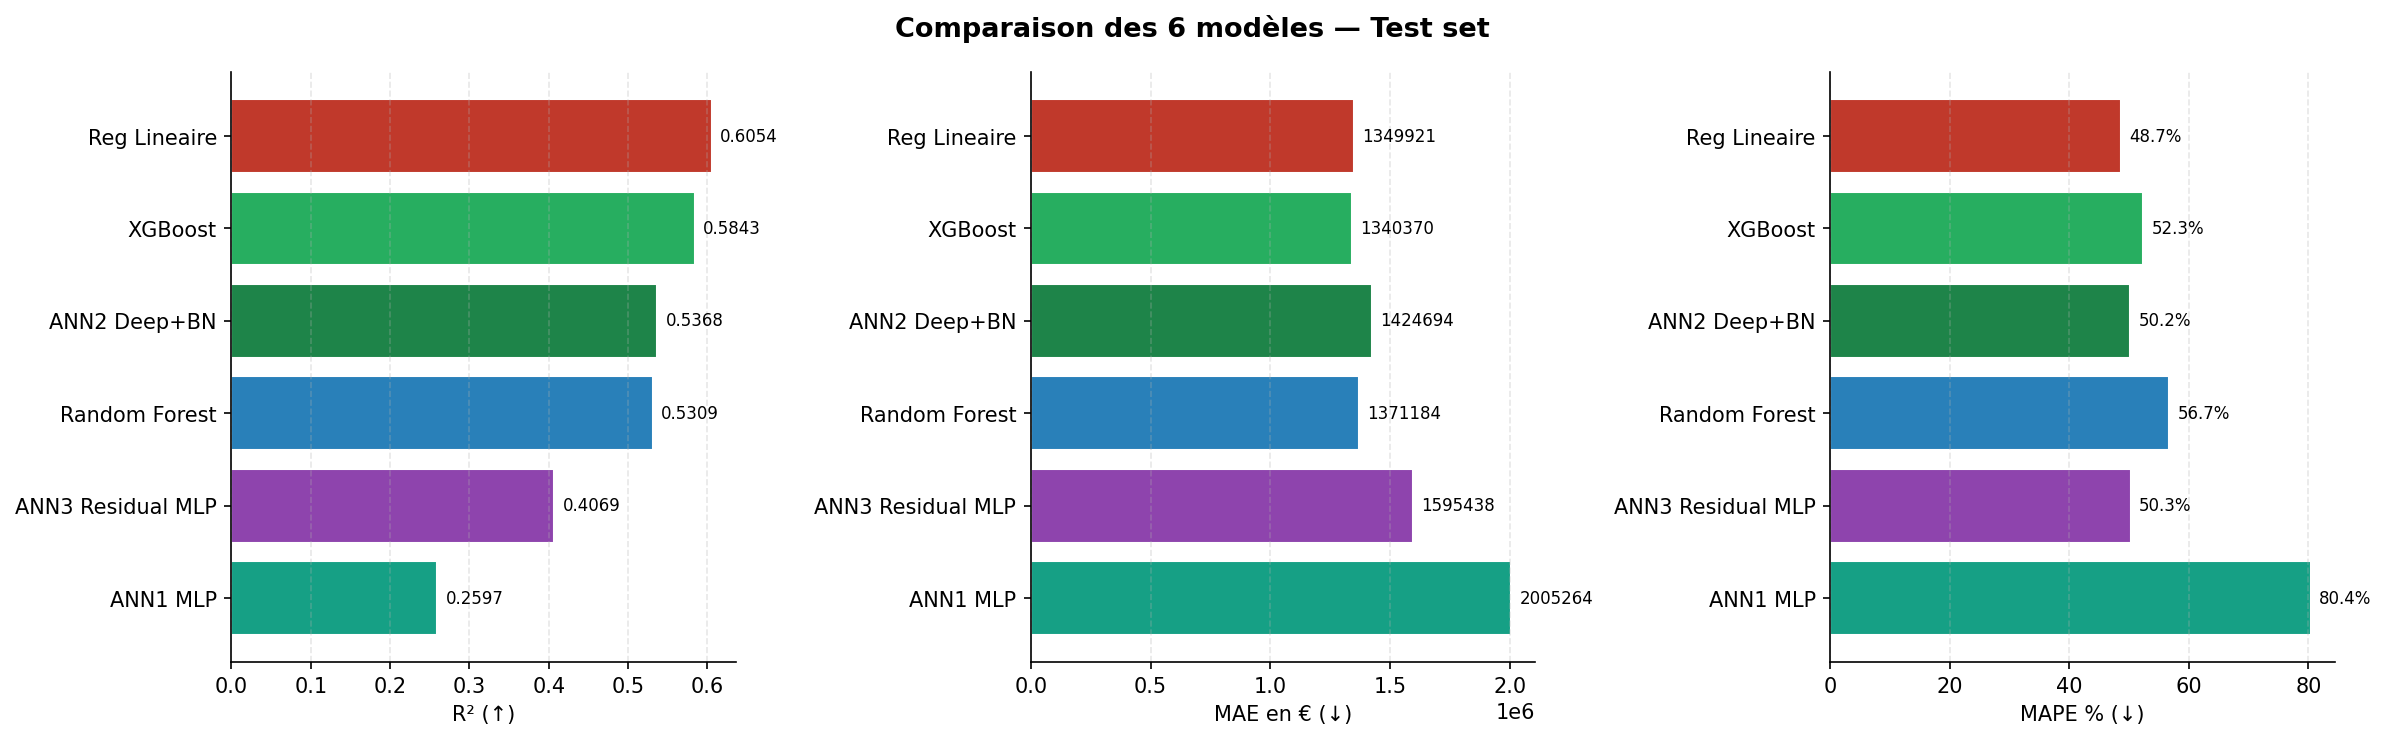
\includegraphics[width=0.9\textwidth]{results_comparison.png}
\caption{Comparaison des performances des 6 modèles (R², MAE, MAPE)}
\label{fig:results_comparison}
\end{figure}

\subsection{Analyse des hyperparamètres}

\begin{figure}[H]
\centering
\begin{minipage}{0.45\linewidth}
\centering
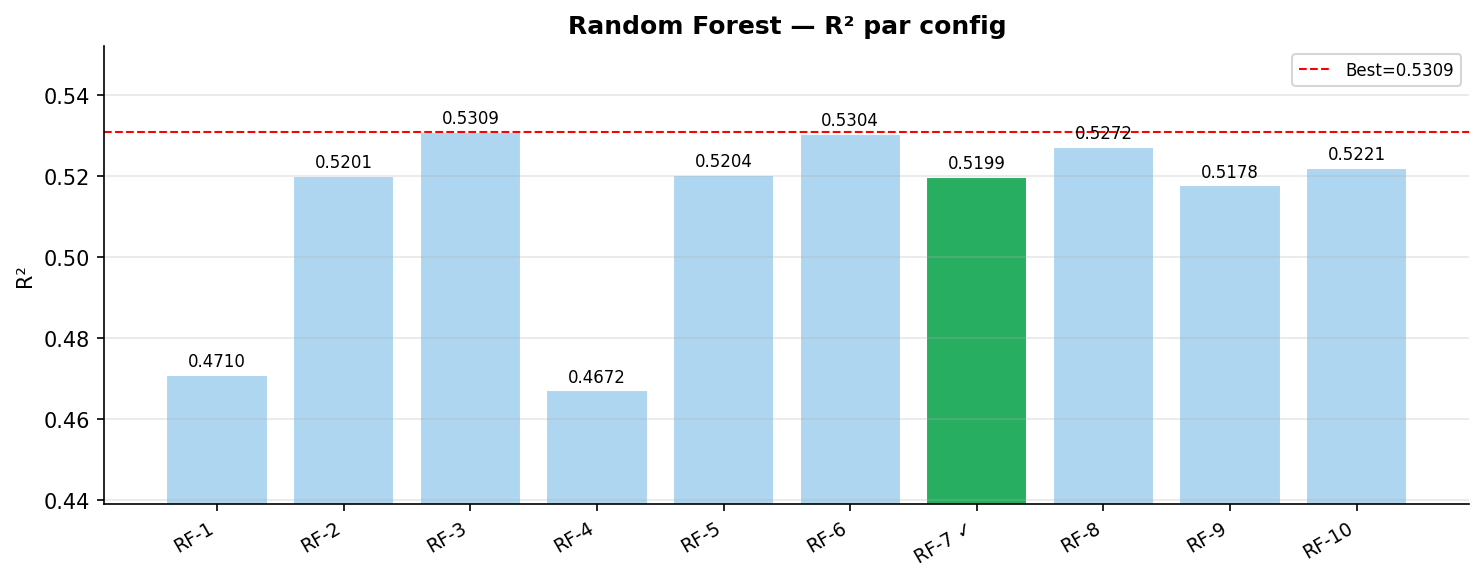
\includegraphics[width=\linewidth]{hyperparam_rf.png}
\caption{Random Forest - Impact des hyperparamètres}
\end{minipage}
\hfill
\begin{minipage}{0.45\linewidth}
\centering
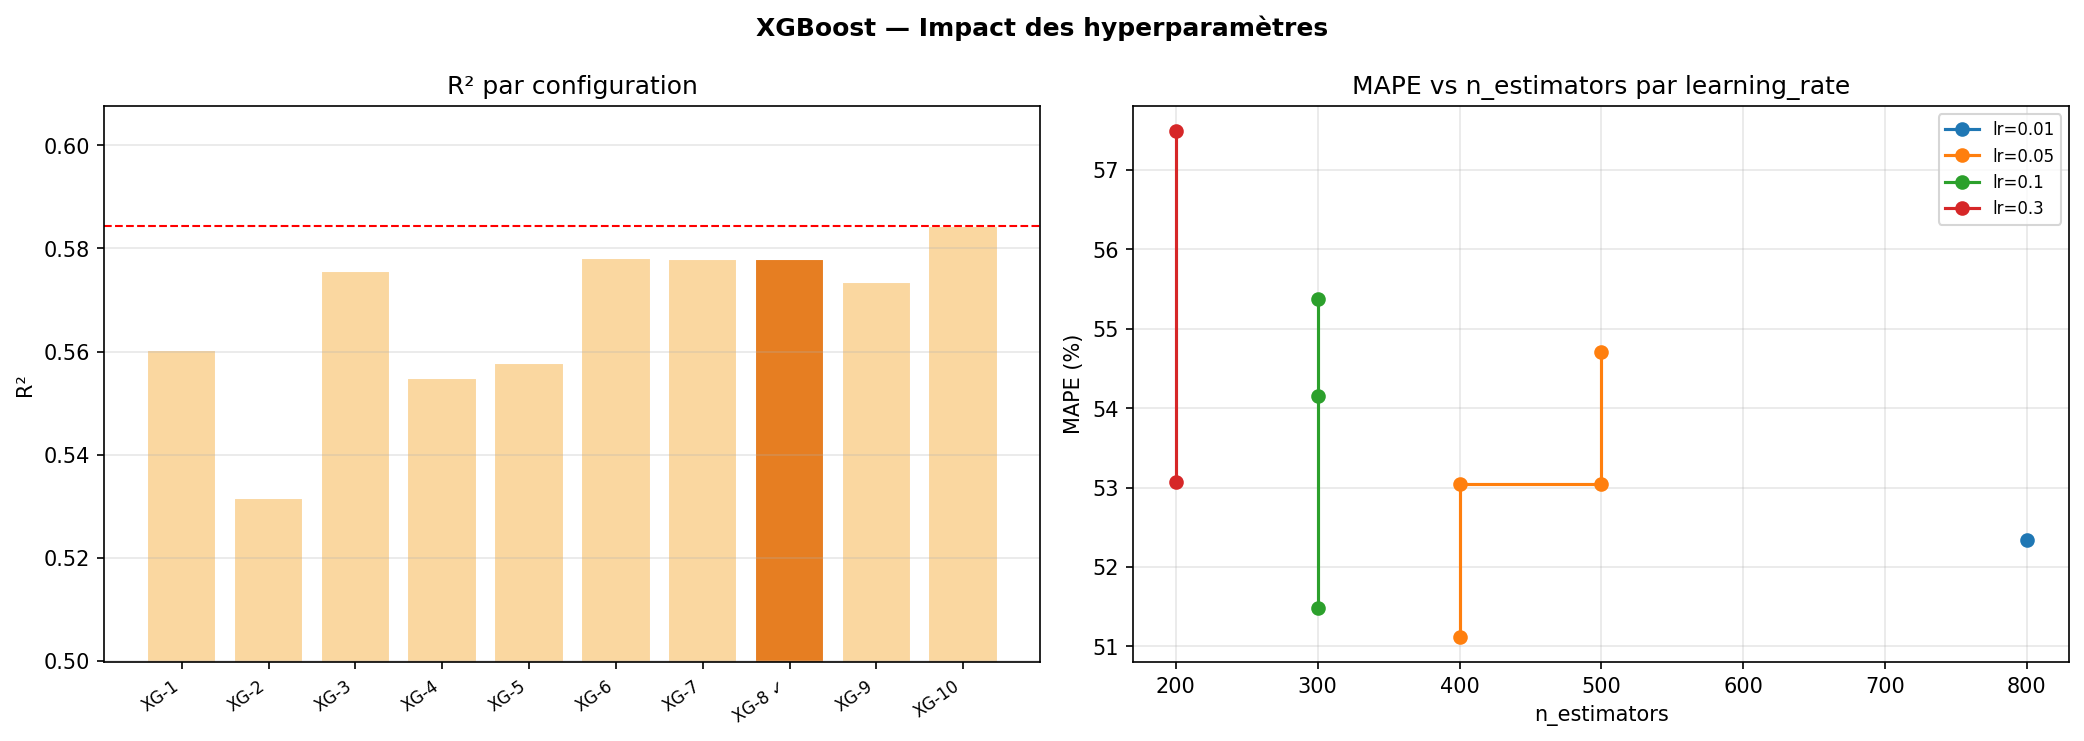
\includegraphics[width=\linewidth]{hyperparam_xgb.png}
\caption{XGBoost - Impact des hyperparamètres}
\end{minipage}
\end{figure}

\begin{figure}[H]
\centering
\begin{minipage}{0.45\linewidth}
\centering
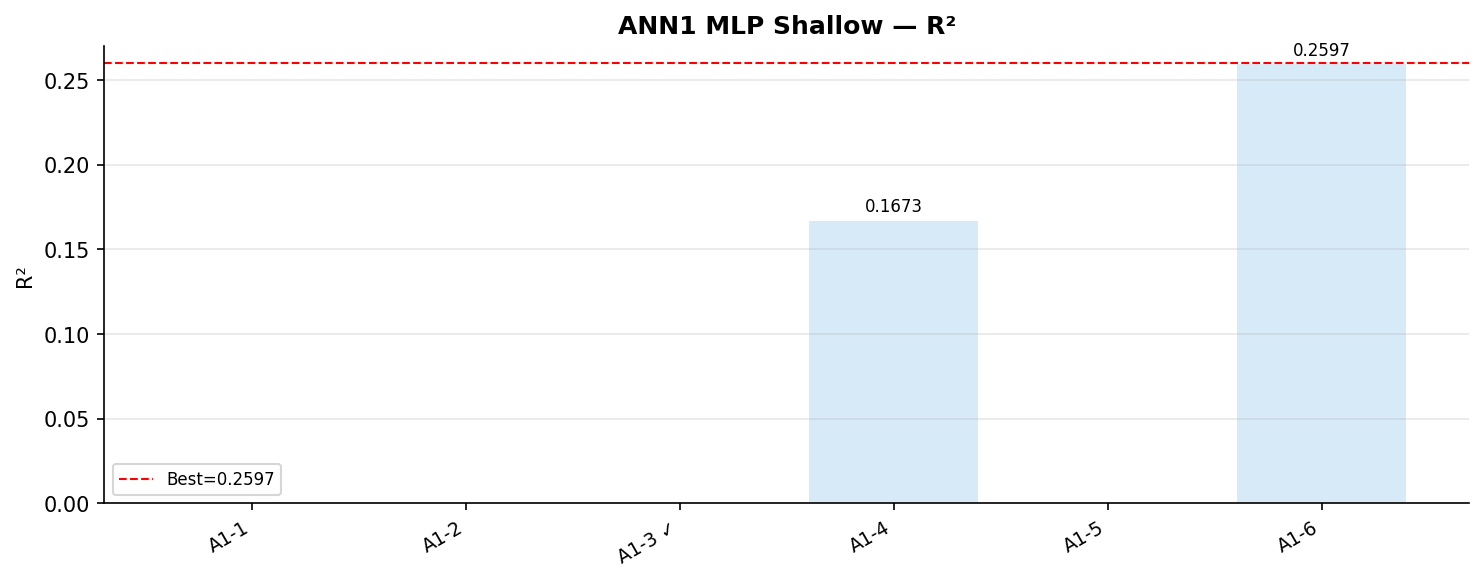
\includegraphics[width=\linewidth]{hyperparam_ann1.png}
\caption{ANN1 MLP Shallow - Impact des hyperparamètres}
\end{minipage}
\hfill
\begin{minipage}{0.45\linewidth}
centering
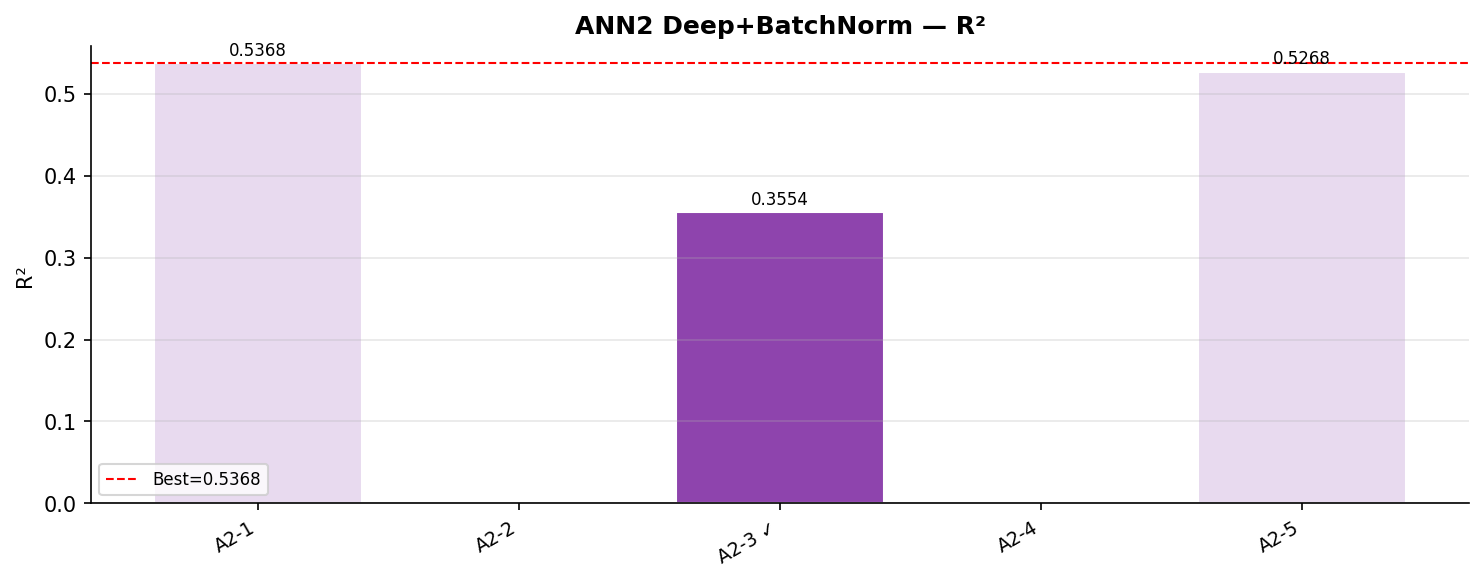
\includegraphics[width=\linewidth]{hyperparam_ann2.png}
\caption{ANN2 Deep+BN - Impact des hyperparamètres}
\end{minipage}
\end{figure}

\begin{figure}[H]
\centering
\begin{minipage}{0.45\linewidth}
\centering
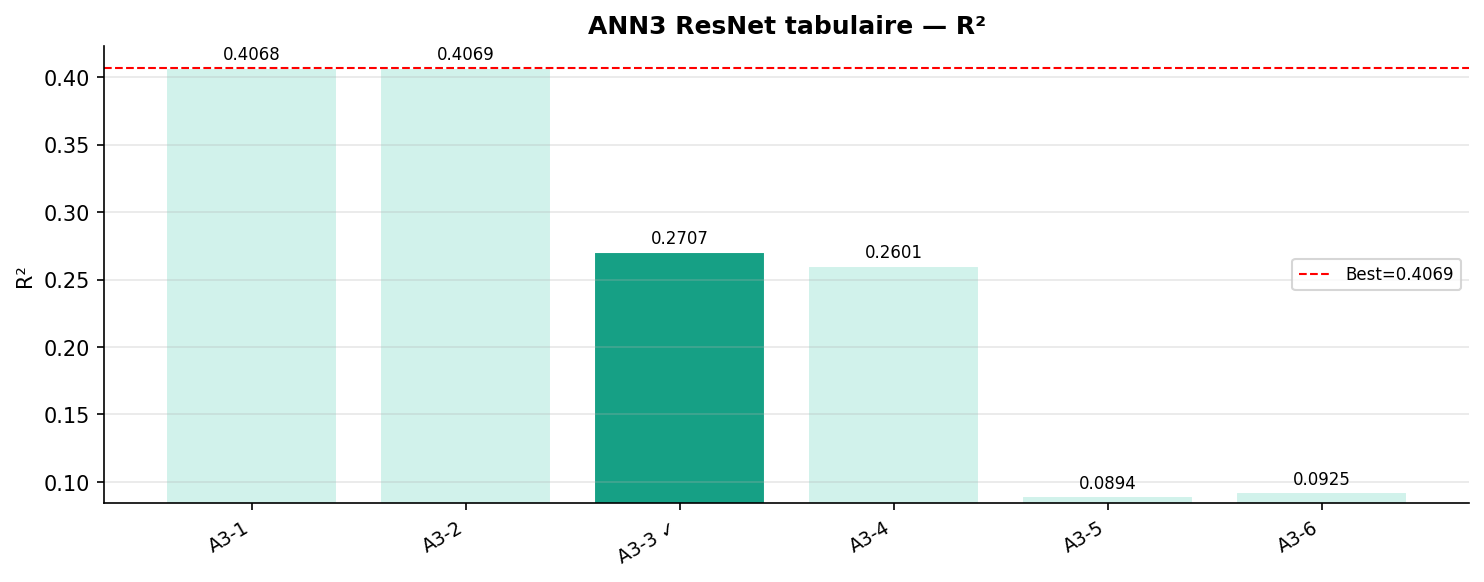
\includegraphics[width=\linewidth]{hyperparam_ann3.png}
\caption{ANN3 Residual MLP - Impact des hyperparamètres}
\end{minipage}
\hfill
\begin{minipage}{0.45\linewidth}
\vspace{1.5cm}
\end{minipage}
\end{figure}

\subsection{Analyse des prédictions}

\begin{figure}[H]
\centering
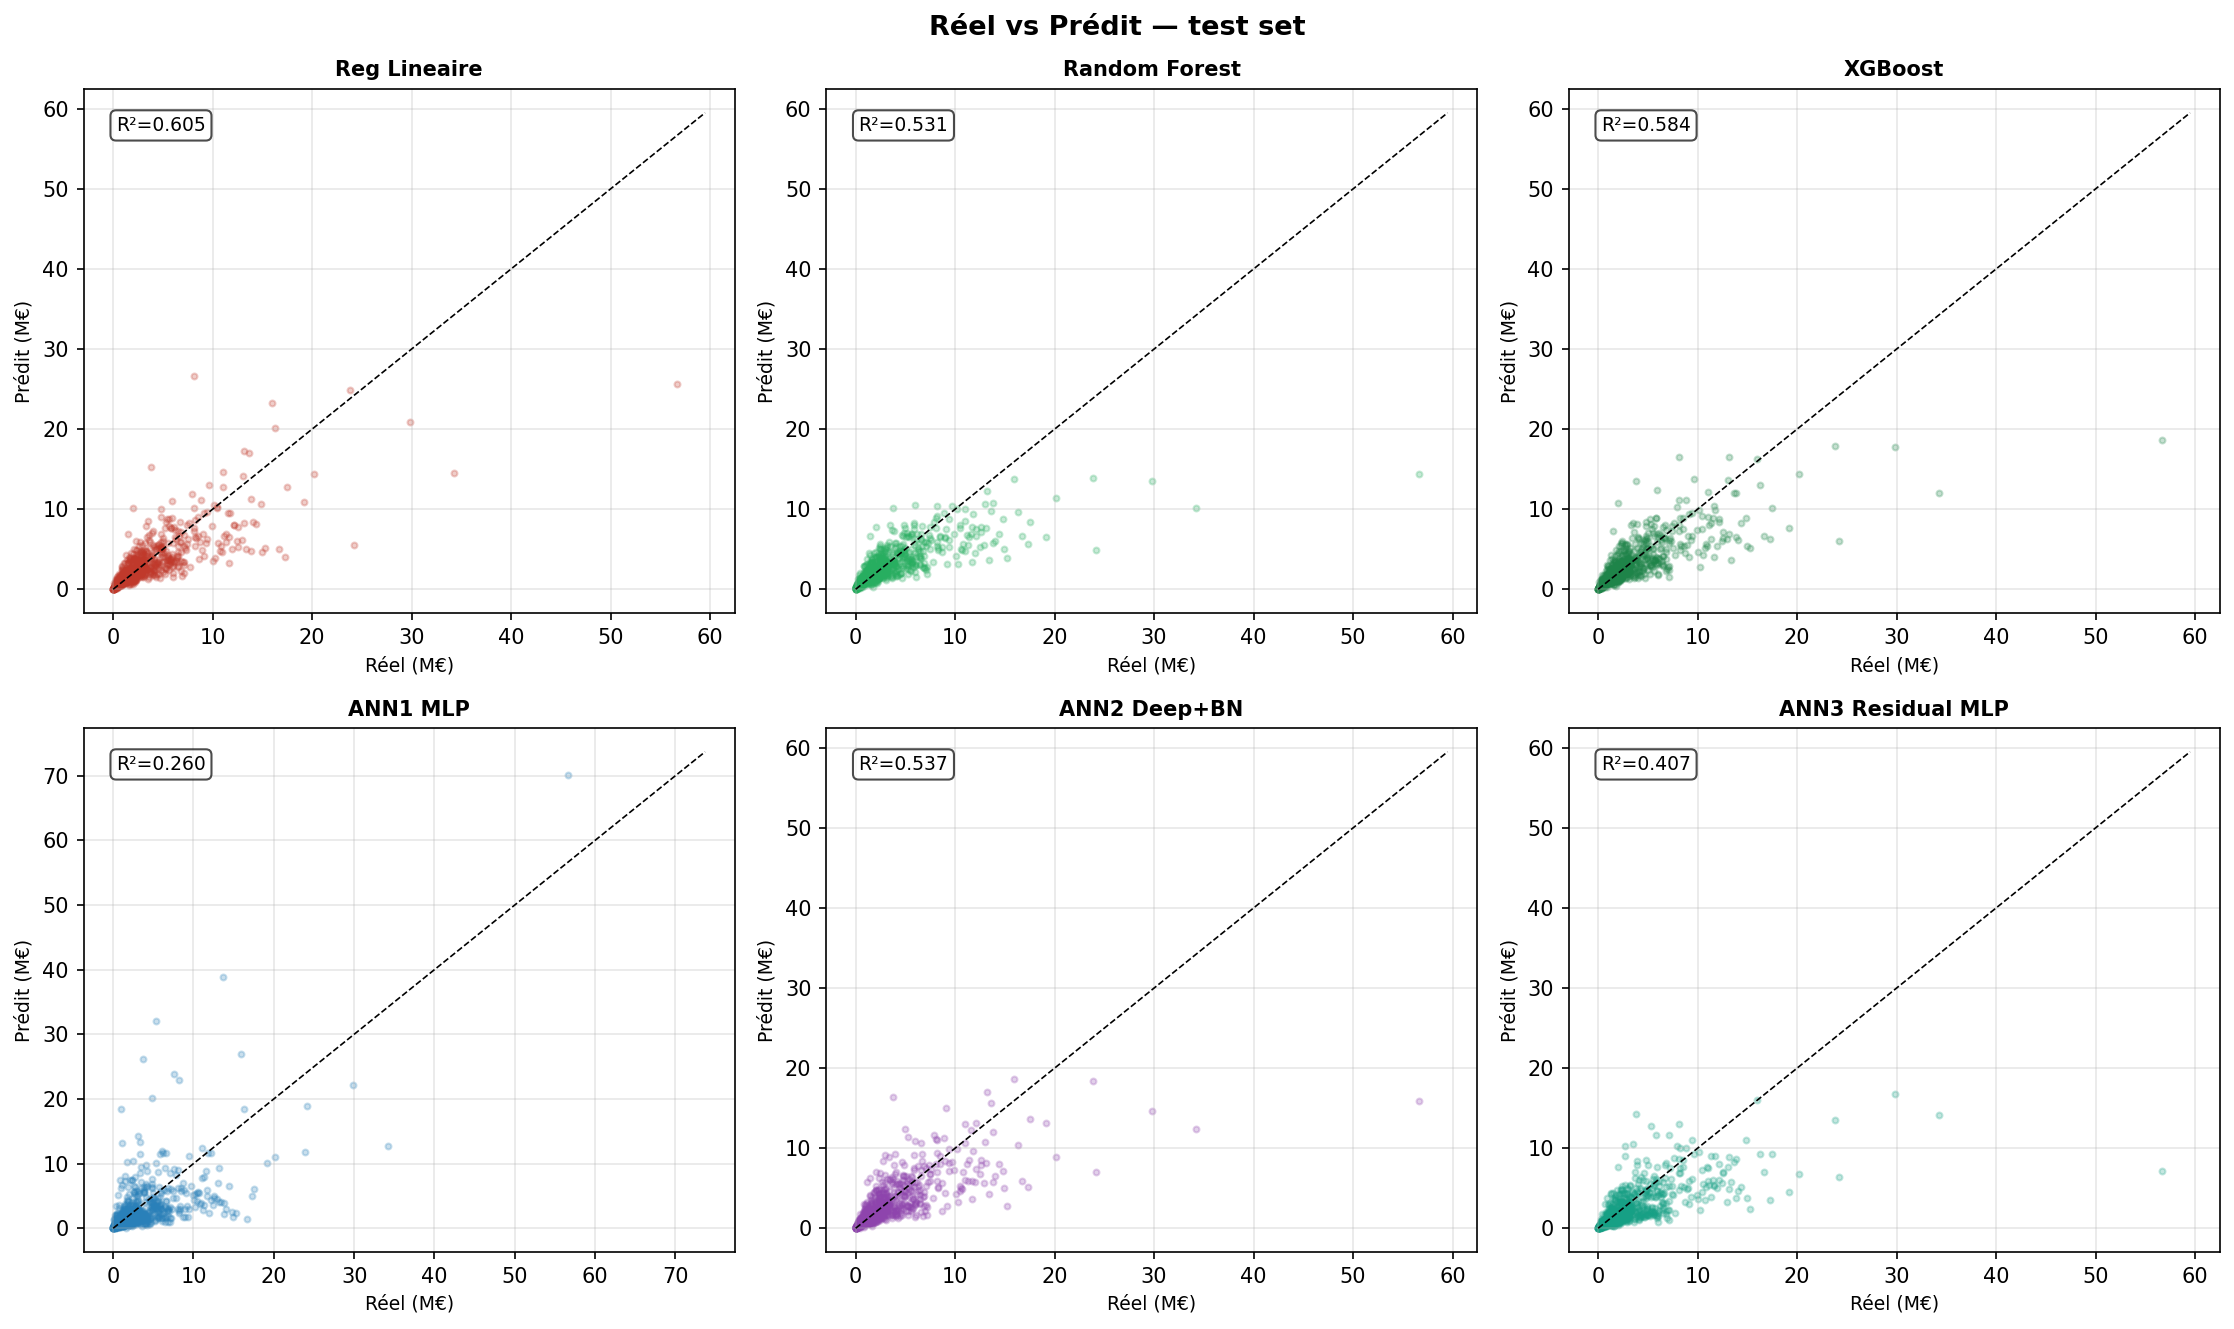
\includegraphics[width=0.9\textwidth]{predictions_scatter.png}
caption{Valeurs prédites vs valeurs réelles (échelle log)}
\label{fig:predictions_scatter}
\end{figure}

Ces visualisations permettent de mieux comprendre le comportement de chaque modèle
et d'identifier les zones où les prédictions sont les plus précises ou les moins précises.

% ============================================================================
% FIN DU DOCUMENT
% ============================================================================

\end{document}